
\documentclass[a4paper,twoside,12pt,nochapterprefix]{scrbook}

% ADDITIONAL PACKAGES ADDED BY ME
\usepackage{listings}
\usepackage[utf8]{inputenc}
\usepackage[usenames,dvipsnames]{color}     
\usepackage{booktabs}
\usepackage{diagbox}
\usepackage{dirtytalk}
\usepackage{breakcites}

%\usepackage{rotating}
%\usepackage{fontspec}

\newcommand{\specialcell}[2][c]{%
\begin{tabular}[#1]{@{}l@{}}#2\end{tabular}}


\lstset{
    alsoletter=?!-><=[]|,
    % literate={>}{{\(\ge\)}}1,
  	% alsodigit=\$\%&*+./:<=>@^_~,
	columns=fullflexible,
	basicstyle=\linespread{0.8}\ttfamily,
	keywordstyle=\color{RoyalBlue}\ttfamily,
	stringstyle=\color{red}\ttfamily,
	commentstyle=\color{ForestGreen}\ttfamily,
	tabsize=4,
	frame=single,
	literate=%
    {�}{{\"O}}1
    {�}{{\"A}}1
    {�}{{\"U}}1
    {�}{{\ss}}1
    {�}{{\"u}}1
    {�}{{\"a}}1
    {�}{{\"o}}1
}

\lstdefinelanguage{PuzzleScript}{%
  alsoletter={v,^,<,>,-,+},
  keywords=[1]{OBJECTS, LEGEND, SOUNDS, COLLISIONLAYERS, RULES, WINCONDITIONS, LEVELS, GENERATION},
  keywordstyle=[1]\color{RoyalBlue}\ttfamily\bfseries,
  keywords=[2]{Player,Wall,Background,Crate,Target,Key,Door,UP,DOWN,LEFT,RIGHT},
  keywordstyle=[2]\color{RoyalBlue}\ttfamily,
  keywords=[3]{->,+},
  keywordstyle=[3]\color{Red}\ttfamily\bfseries,
  keywords=[4]{>,<,v,^},
  keywordstyle=[4]\color{ForestGreen}\ttfamily\bfseries,
  keywords=[5]{up,down,left,right,action,no,No},
  keywordstyle=[5]\color{ForestGreen}\ttfamily,
  morecomment=[l][\color{Gray}]{==},
  morecomment=[s]{(}{)},
  morestring=[b]",
  morestring=[b]',
  alsoother={\,0"},
  sensitive=true,
  literate=*{"}{,}{1}
}
\lstset{
language=PuzzleScript
}

%\usepackage[symbol]{footmisc}

%\@addtoreset{footnote}{page}


% \renewcommand*{\footnotelayout}{\small\tffamily}
% \renewcommand{\thefootnote}{\fnsymbol{footnote}}

%\renewcommand*{\thefootnote}{\alph{footnote}}

\usepackage{amsmath,amssymb,amsthm}
\usepackage[footnotesize,sl,SL,hang,tight]{subfigure}  % helpful package for aligning figures next to each other
\usepackage{longtable} % tables over several pages
\usepackage[font={small,sl},hang,labelfont=bf]{caption} % configure captions
\usepackage{booktabs} % publication quality tables for LaTeX
%\usepackage{showkeys} % shows the labels above the references for easier development

\ifpdfoutput{%
	\usepackage[pdftex]{graphicx}
	\usepackage[]{pdfpages} %for including full pdf pages
}{%
	\usepackage{graphicx}
}
\usepackage{epstopdf}
\epstopdfsetup{update} % only regenerate pdf files when eps file is newer

\usepackage{rotating} % rotate figures

\usepackage[headinclude]{scrpage2}

% Font packages:
\usepackage{times}
\usepackage{helvet}   % sets sans serif font
\usepackage[T1]{fontenc}

%PDF hyperref config
\ifpdfoutput{%
	\usepackage[pdftex,
		a4paper,
		bookmarks,
		bookmarksopen=true,
		bookmarksnumbered=true,
		pdfauthor={My Name},       % FILL THIS IN PROPERLY
		pdftitle={Thesis Title},   % FILL THIS IN PRPERLY
		colorlinks,
		linkcolor=black,
		citecolor=black,
		filecolor=black,
		urlcolor=black,
		anchorcolor=black,
		menucolor=black,
		breaklinks=true,
		pageanchor=true,
		plainpages=false,
		pdfpagelabels=true]{hyperref}
}{}

\ifpdfoutput{%
	\pdfcompresslevel=9
	\pdfoutput=1
	\DeclareGraphicsExtensions{.pdf,.png}
}{}

\bibliographystyle{acmsiggraph}



% A4
%
\topmargin -0.5in
\textheight 9.3in
\textwidth 6.3in
\oddsidemargin 0.18in
\evensidemargin -0.22in
\parskip 0.1in
\parindent 0in

\renewcommand{\arraystretch}{1.5}
\renewcommand{\baselinestretch}{1}

% !TEX root = ../thesis.tex

% TO DO search symbol
\newcommand{\TODO}{\mbox{\large\bf TO DO}}
\newcommand{\REFR}{\mbox{\large\bf REFR}}

%  Terminates current page and paragraph, makes sure next page starts on
%  an odd-number, and generates a completely blank page, without page markers,
%  if necessary.
\newcommand{\clearemptydoublepage}{\newpage{\pagestyle{empty}\cleardoublepage}}


% !TEX root = ../thesis.tex

% Stripped from acm siggraph bst and cls
\makeatletter

% no labels in bibliography.
\def\@biblabel#1{}

\newlength{\bibhang}
\setlength{\bibhang}{1em}

% Change in-bibliography biberence style
\iffalse
\def\thebibliography#1{%
  \section*{%
    \bibname\@mkboth{\sl\uppercase{\bibname}}{\sl\uppercase{\bibname}}}
  \list{\relax}{\setlength{\labelsep}{0em}
                \setlength{\itemindent}{-\bibhang}
                \setlength{\leftmargin}{\bibhang}}
  \def\newblock{\hskip .11em plus .33em minus .07em}
  \sloppy\clubpenalty4000\widowpenalty4000
  \sfcode`\.=1000\relax}

\fi




% Not sure what this does...
%\def\@citex[#1]#2{\if@filesw\immediate\write\@auxout{\string\citation{#2}}\fi
%  \def\@citea{}\@cite{\@for\@citeb:=#2\do
%    {\@citea\def\@citea{; }\@ifundefined
%      {b@\@citeb}{{\bf ?}\@warning
%      {Citation '\@citeb' on page \thepage \space undefined}}%
%{\csname b@\@citeb\endcsname}}}{#1}}

% Change in-document citation styles
\let\@internalcite\cite
\def\cite{\def\citename##1{##1}\@internalcite}
\def\shortcite{\def\citename##1{}\@internalcite}

\makeatother


\begin{document}

%% Define leading chapter pages
%
% !TEX root = ../thesis.tex

\addtokomafont{chapter}{\setlength{\parskip}{190pt}}   % SEVERE HACK to keep spacing to chapter art work
%\addtokomafont{chapter}{\rmfamily}        % remove this if you prefer sans-serif section titles
%\addtokomafont{section}{\rmfamily}        % remove this if you prefer sans-serif section titles
%\addtokomafont{subsection}{\rmfamily}     % remove this if you prefer sans-serif section titles
%\addtokomafont{subsubsection}{\rmfamily}  % remove this if you prefer sans-serif section titles
%\addtokomafont{paragraph}{\rmfamily}      % replace by \sffamily if you prefer sans-serif para titles
\addtokomafont{paragraph}{\sffamily}

\def\mychpstyleintl{%
{\noindent\setlength{\tabcolsep}{0pt}\setlength{\arrayrulewidth}{2pt}%
\begin{tabular}{c}
\\[100pt]
\begin{tabular}{lr}
\begin{tabular}{p{0.6\linewidth}}
\\
\end{tabular}
&
\begin{tabular}{p{0.4\linewidth}}
\rightline{{%
\sffamily%
\fontseries{bx}%
\fontshape{n}%
\fontsize{100}{120}%choose baselineskip to be 1.2 times font size
\selectfont
\thechapter}}
\end{tabular}
\end{tabular}\\[300pt]
\end{tabular}
}}

\newpagestyle{mychapterpagestyle}{{\protect\mychpstyleintl}{\protect\mychpstyleintl}}{}
\newpagestyle{myappendixpagestyle}{{\protect\mychpstyleintl}{\protect\mychpstyleintl}}{}
%%

%% macros e.g.
\newcommand{\mfytext}[0]{my fancy text}

%refs
\newcommand{\chpref}[1]{Chapter \ref{#1}}
\newcommand{\secref}[1]{Section \ref{#1}}
%\newcommand{\equref}[1]{Equation \ref{#1}} %better use builtin \eqref{}
\newcommand{\figref}[1]{Figure \ref{#1}}
\newcommand{\tabref}[1]{Table \ref{#1}}
\newcommand{\apxref}[1]{Appendix \ref{#1}}
%%

%% Replace this by your own design of a title page
%
%\title{Thesis Title}
%\author{My Name}
%\date{September 2042}
%\maketitle
%\clearemptydoublepage
% --- selfmade version ----
\begin{titlepage}
	\topmargin 1.0cm
	\oddsidemargin 0.0cm
	\evensidemargin 0.0cm
	%\textwidth 6.5in
	\centering
	\Huge
	\vspace{3.0cm}
	\textbf{\textsf{Mixed-Initiative Methods for Designing Sokoban-like Puzzles}} \\[2.0cm]
	\includegraphics*[width=0.8\textwidth]{figures/titleimage} \\ % TITLE IMAGE - replace by attractive and representative images from your thesis
	\vspace{3cm}
	\sffamily
	\Large
	Kevin De Keyser
	\\[0.8cm]
	\large
	Bachelor Thesis % Bachelor Thesis
	\\
	July 2019
	\\[1.3cm]
	\emph{Supervisors:}\\
	Dr.\ Anna Maria Feit\\ 					% The name of the thesis supervisor
	Prof.\ Dr.\ Otmar Hilliges		% The supervising professor
	\vfill
	\includegraphics*[height=0.8cm]{figures/eth_logo_kurz_pos.eps} \hfill
	\includegraphics*[height=0.8cm]{figures/logo-ait}
	\vspace{3.4cm}
\end{titlepage}
\clearemptydoublepage
%%

\pagenumbering{roman}
\setcounter{page}{1}

% !TEX root = ../thesis.tex

\chapter*{Abstract}

Successful puzzle games have both been designed completely by hand and completely through computer generation. Can value be derived from combining both in a mixed-initiative fashion?
The aim of this thesis was to develop interactive tools that bring 'genuine value' to the process of puzzle game design, by which interactions are meant, which the designer could not easily attain through direct manipulation.
For this purpose we created MixedAim which is a tool that can give level suggestions   

. Through a qualitative user study we identified design approaches  designers employed to create puzzle games and analysed in which ways interactions with MixedAim supported these approaches.

We believe to have found 3 modes of designing a level.

Furthermore, we modelled the adaption of the designer towards the tool and analysed which adaptions were beneficial and why.

Finally, we found that these interactions should best be viewed as a set of tools with which one can design a level and not as a panacea   

 as giving a few more approaches to puzzle design but are not a panacea.


% Furthermore, we found that MixedAim, and for that matter other mixed-initiative tools, should be viewed as providing a few approaches for designing puzzles but they are not a panacea for design. 


% Concerns about creating easy levels.



\cleardoublepage
\chapter*{Zusammenfassung}

Diese Arbeit beschäftigt sich mit der Entwicklung einer neuartigen Beispielausarbeitung. Wir untersuchen die Anforderungen, die sich für eine allgemeine Vorlage ergeben, die innerhalb der \LaTeX-Textverarbeitungsumgebung verwendet werden kann. (Und so weiter und so fort\dots) Die Zusammenfassung sollte nicht länger als eine halbe Textseite sein!


%-----------------------------------------------------------------------------------------------
%include task description here:
\cleardoublepage
%\includegraphics[viewport=3cm 0cm 20cm 27.5cm]{task_description} %better use includepdf below!
%\includepdf{task_description}
\cleardoublepage
%-----------------------------------------------------------------------------------------------

%include acknowledgment here:
%\include{./chapters/acknowledgment}

\tableofcontents

\cleardoublepage
\phantomsection
\addcontentsline{toc}{chapter}{List of Figures}
\listoffigures

\cleardoublepage
\phantomsection
\addcontentsline{toc}{chapter}{List of Tables}
\listoftables
\cleardoublepage

\pagenumbering{arabic}
\renewcommand*{\chapterpagestyle}{mychapterpagestyle}
\renewcommand*{\chapterformat}{} % show chapter titles only (no numbers)
% \setchapterpreamble[o]{...}  unfortunately does not move the \chapter output downwards

% ---- MAIN PART ----

% !TEX root = ../thesis.tex

% set counter to n-1:
\setcounter{chapter}{0}

\chapter{Introduction}
A puzzle in the context of video games is conventionally any problem that the player has to solve inside the video game to progress, be it a visual, an auditorial or a dialogue-based problem, and should not be confused with 'Jigsaw puzzles' which are just one possible puzzle type.

Most puzzle games serve as a recreational activity, although they are increasingly used for other purposes, such as for \href{https://www.theguardian.com/technology/2014/jan/25/online-gamers-solving-sciences-biggest-problems}{the gamification of jobs} \cite{TheGuardian}, for \href{https://www.euclidea.xyz}{reframing educational problems as puzzle games} \footnote{\url{https://www.euclidea.xyz}} (also \cite{Lee2014}) or for using them as \href{http://www.gvgai.net}{training grounds for general artificial intelligence} \cite{Perez2014}.

To get a better picture of why people play puzzle games, we conducted a need-finding survey \ref{needfindingq1} where we asked participants, amongst other questions, why they like to play puzzle games. We received the following responses:

\textit{ "to feel smart", "experience aha-moments", "increased spatial reasoning skills", "to get into the state of flow", "because it is fun"}.

Prior literature found similar reasons. In \cite{Kangas2017}, Kangas analyzed the pleasure of puzzles in the context of adventure games and highlights Csikszentmihalyi's work on flow \cite{Csikszentmihalyi}, also referencing flashes of insights and a cycle of suspense and relief as key reasons for player engagement. If the puzzles are too difficult, the player gets frustrated, when the puzzles are too easy, the player gets bored. It is only when the difficulty is just right that the player can get immersed in the challenge and derive pleasure from playing the puzzle. Kangas particularly mentions that puzzles can also be used as part of a broader experience and can help with immersing the player inside the game world by putting them in a state of flow.

 % The correlation between 'difficult for a human' and 'difficult for the program' are still...


%We had a hunch that difficult levels also tend to be fun/interesting.

%We leave the judging of fun to the user and try to optimize for difficult levels based on the guidance of the user. In this way, we exploit both the strengths of the designer and the machine in a mixed-initiative fashion.


\section{Sokoban}

Video games allow for puzzles that cannot easily be played on pen-and-paper (contrary to say Sudoku) since they can have an interactive element to them. A video game could, for example, hide information from the player and only reveal it at a later stage, change the game state while the player tries to solve the level or make it a lot easier to trial-and-error solutions.


One of the arguably first puzzle video games to take advantage of this was Sokoban invented by Hiroyuki Imabayashi in 1981. Inspired by warehouses, in Sokoban, the player controls a person whose job is to push crates/boxes onto storage locations (see image). Since its inception Sokoban has spawned \href{http://www.onlinespiele-sammlung.de/sokoban/list-of-sokoban-games.php}{hundreds of successors} \footnote{\url{http://www.onlinespiele-sammlung.de/sokoban/list-of-sokoban-games.php}} and has inspired countless others. It has also been a popular choice for research, a quick search on Google Scholar reveals roughly 2'040 papers that mention Sokoban at the time of writing, hinting at its popularity.

\begin{figure}[h]
    \centering
    \setlength{\tabcolsep}{0.0130\linewidth}
    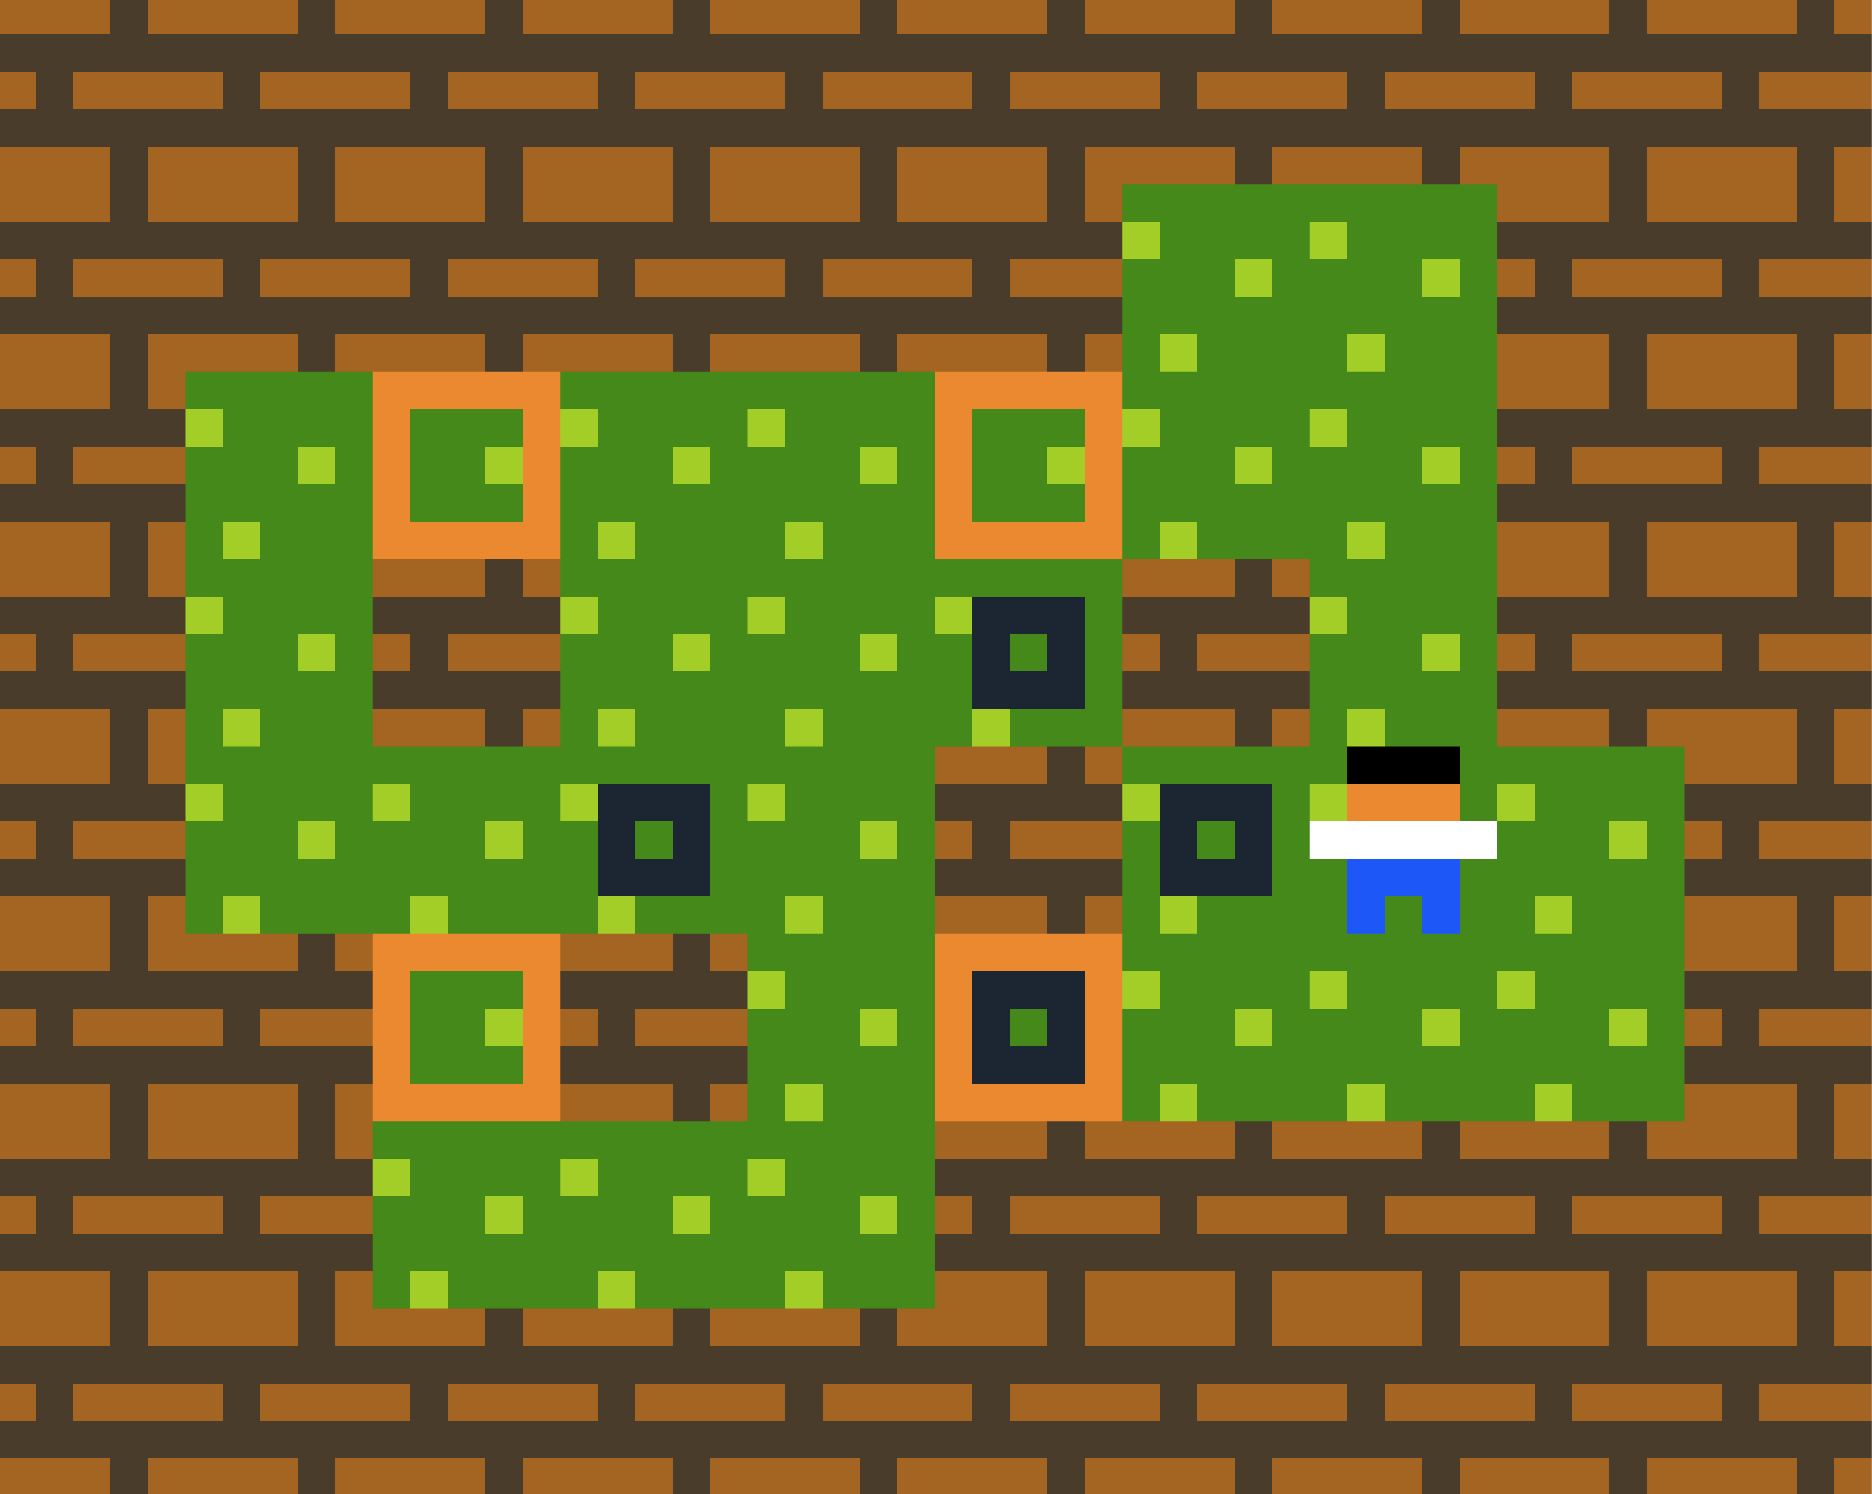
\includegraphics[width=0.487\linewidth]{figures/45minslevel.png}
    
    %\begin{tabular}{@{}cc@{}}
    %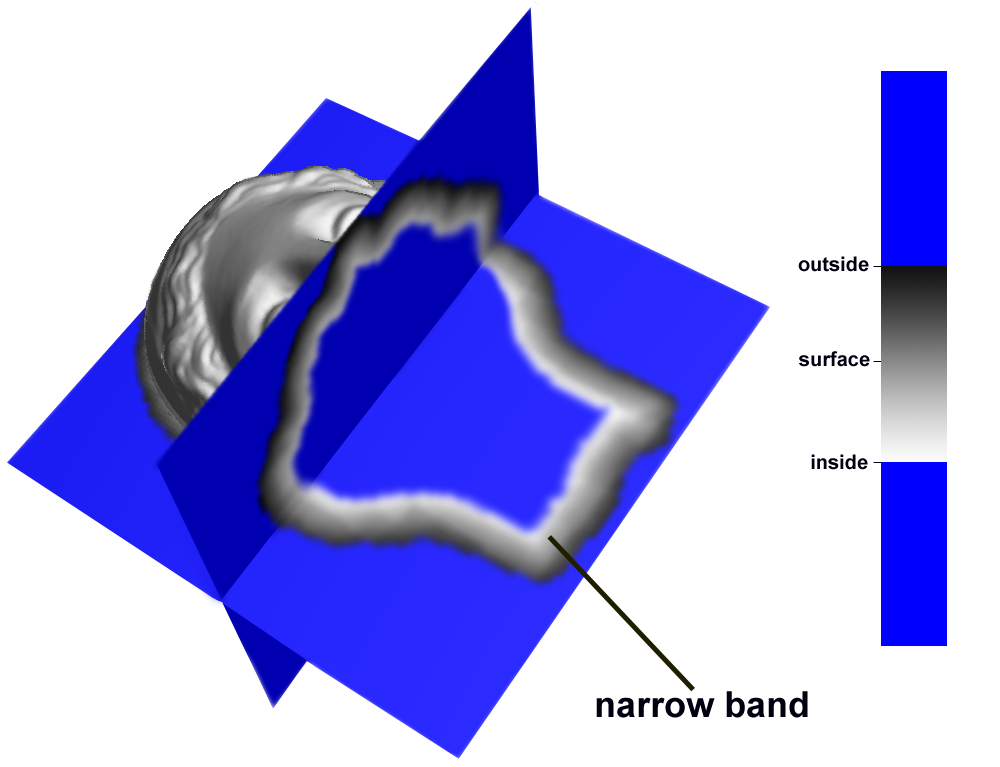
\includegraphics[width=0.487\linewidth]{figures/IgeaNarrowBand}&
    %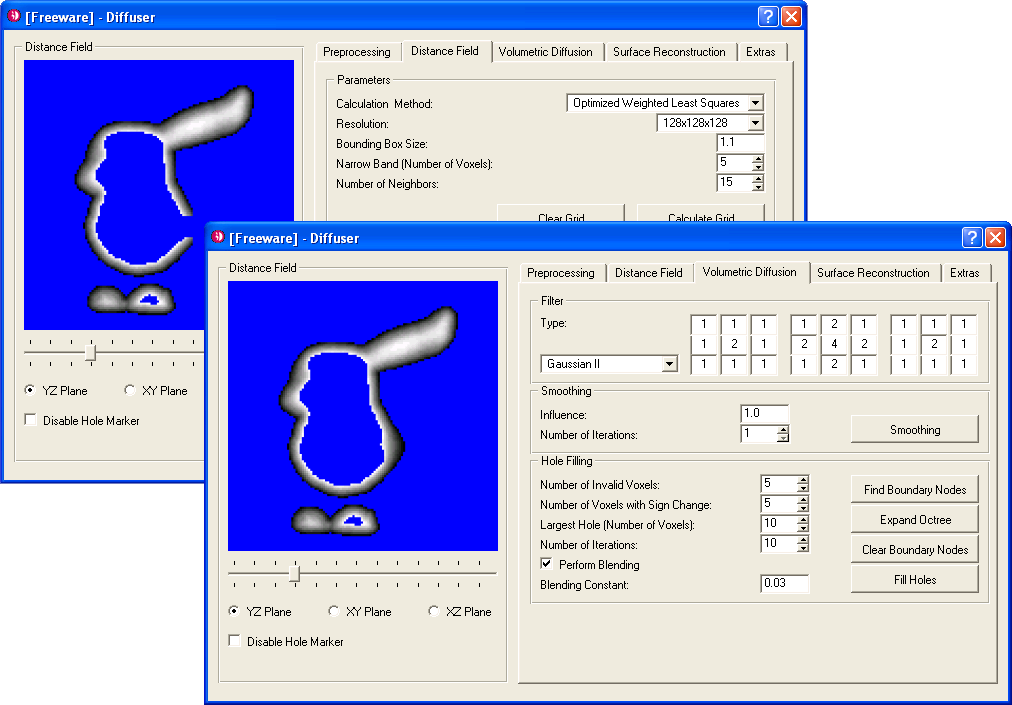
\includegraphics[width=0.487\linewidth]{figures/voldiff_ui}\\
    %(a)&(b)\\
    %\end{tabular}
    \caption[43 Minute Sokoban level]{A Sokoban level taken from \cite{Pelanek2011} %
      \label{fig:43minsfig}}
\end{figure}

Solving a Sokoban level requires much trial-and-error, making it less suited to be played on pen-and-paper. To get a sense of the difficulty, according to \cite{Pelanek2011}, the puzzle in Figure \ref{fig:43minsfig} already takes a median solving time of 43 mins.

For this reason, it only seems natural for designers to correspondingly use tools outside of pen-and-paper when designing Sokoban levels.  
From our need-finding survey \ref{fig:needfindingq3} we know that in practice puzzle designers use a diverse number of approaches and tools. Commercial games have likewise been made with a diverse set of approaches ranging from fully-automated approaches (like Donnantuoni's \href{https://marcosd.itch.io/dispontibus}{Dis Pontibus}\footnote{\url{https://marcosd.itch.io/dispontibus}}) to approaches which are almost exclusively based on pen-and-paper (like Blow's \href{http://the-witness.net}{\url{The Witness}}\footnote{\url{http://the-witness.net}}). Our need-finding survey also, however, showed that designers are open to trying out new interactive methods to add to their design process.

One such tool for designing puzzle games is \href{https://www.puzzlescript.net}{PuzzleScript}\footnote{\url{https://www.puzzlescript.net}} from \href{https://www.increpare.com}{Stephen Lavelle}, a tool all 5 participants from the need-finding interview use, which comes with a level editor (a graphical tool to place the blocks easily) and a run mode (a mode to play-test the designed level). Apart from that it does not provide further interactions to create puzzles for puzzle design.


\section{Aim of the study}

This brings us to the aim of this study, which is to develop interactive tools that bring 'genuine value' to the process of puzzle game design, by which interactions are meant, which the designer could not easily attain through direct manipulation (say by using a level editor). For this purpose, we created a mixed-initiative creative interface (MICI) for PuzzleScript called \textit{MixedAim} that allows a tight interaction between the designer and the tool when creating Sokoban-like puzzle games. The reason we choose PuzzleScript was so we could support a broader range of games without giving up much functionality.

\cite{Koch} have shown that computer tools which are both controlled by the human and by the machine, so-called mixed-initiative tools, can be employed successfully to creative tasks like designing moodboards. Moodboards are a collection of images meant to communicate a theme and inspire people who see it. The tool suggests images based on the already designed moodboard, and the user can steer the suggestions using three buttons `more like this', `not this one' and `surprise me'. Similarly, puzzle games are a collection of levels intended to be fun and designed to make the player better at solving them. Our tool MixedAim gives suggestions on how to change a level and allows designers to change the type of suggestions via buttons like `modify this level more' or `change only the walls of this level'. Furthermore, it allows experienced designers to specify their own ways of steering suggestions explicitly.
MixedAim then tries to suggest interesting levels based on these constraints to the user. But what makes a good suggestion? 


\section{Formal theory of fun}
The puzzle games we concern ourselves with are comparable to formal systems, the keyword being \textit{formal} meaning that every state and action inside the game is \textit{well-defined}.
In this analogy, the player starts from a well-defined starting configuration/state (theorem), applies inputs to the puzzle game which lead to well-defined state changes (derivation rules) to achieve a possible well-defined goal configuration (axiom). Usually, puzzle games can have multiple goal states, but they only have a single starting configuration.

In the literature of puzzle games \cite{RulesOfPlay} these well-defined state changes (derivation rules) are called  \textit{operational mechanics}, i.e., the mechanics which are programmed explicitly into the game to make it function (hence the term operational). While playing the game, the player identifies \textit{constituative mechanics} and starts using them in addition to \textit{operational mechanics} to find a solution. For example, in Sokoban, as soon as a crate is pushed next to the right-most wall, there is no way of pushing the crate back from the wall. 

Usually, people concern themselves with formal systems because solving a formal problem (proving a theorem) has useful implications in the real world. For puzzle games, on the other hand, as we have mentioned, it is not very clear why people solve them and which puzzles are more interesting than others.

The best explanation we have found so far comes from Jurgen Schmidhuber's formal theory of creativity, fun, and intrinsic motivation \cite{Schmidhuber}. In a nutshell, the human player is modeled as a reinforcement learner, and the learning process (in this case identifying constituative mechanics and creating a smarter process for solving a level based on these mechanics) is the human player's fun. This also matches with some of the responses of our need-finding study: \textit{"because it is fun.", "experience aha-moments"}.

In more detail, the human player needs to utilizes a certain amount of energy (both mentally and through interaction with the system) to find a goal state. We call this the \textit{subjective difficulty} or correspondingly the \textit{subjective simplicity}. Measuring the \textit{subjective difficulty} quantitatively is difficult since some players stare at a level for a long time before solving it in one go while others start using pen-and-paper to solve a puzzle. It is a lot easier however to measure the energy/the number of operations of a computer program (or as in Schmidhuber's case a reinforcement learner) has to expend in order to find a solution. Schmidhuber also calls this measure the \textit{subjective momentary simplicity} or \textit{compressibility} or \textit{regularity} or \textit{beauty} depending on the problem/context.

Next, while playing a single level, the human discovers constituative mechanics and new strategies of solving levels with these mechanics. This level of discovery is the \textit{subjective interestingness} of a level. Notice that if a player plays the same level over and over the level will start to be less and less interesting to the player. Again quantifying this is very difficult for humans but can be done easily for computer programs (specifically for learning programs). Schmidhuber measures this by subtracting the \textit{subjective difficulty} before solving the level and after solving the level. This way he quantifies how much the program (usually a reinforcement learning program) has learned from playing a level. Schmidhuber also calls this measure \textit{novelty} or \textit{surprise} or \textit{aesthetic reward} or \textit{aesthetic value} or \textit{internal joy} or simply \textbf{fun}, again, depending on the problem/context.

Unfortunately, reinforcement learning algorithms have not been successfully applied to Sokoban, and, to our knowledge, the best Sokoban solvers are not in any shape or form `learning'. Still, we can measure the difficulty of a level by the number of states an algorithm has to explore in order to find a solution.
Since all fun puzzle games feature difficult levels, we had a hunch that difficulty was a useful measure to design fun games. 

Based on this, our final research question is: How can interactive tools, specifically tools which focus on providing more difficult level suggestions, aid the user in designing puzzle games?
% !TEX root = ../thesis.tex

% set counter to n-1:
\setcounter{chapter}{1}

\chapter{Related Work}
In creative tasks, such as puzzle design, designers do not always know from the start what they are trying to create. This makes it a very difficult task to automate fully (blindly optimizing some difficulty measure can reduce the perceived fun, for example).

\subsubsection{Generating Sokoban Levels}
%This has not stopped people from trying though with various degrees of success. 

Arguably the first group to have written on Sokoban generation is \cite{Science1996}. Here they generate the puzzle game from a preset prototype level which is modified using templates ($2 \times 2$ or larger sequence of blocks) into levels. They then check the solvability of the level using a breadth-first-search and evaluate them based on a few criteria: length of solution, number of changes in directions of pushing \& number of detours in a solution sequence.

\cite{Pelanek2011} did a human case study on Sokoban problem solving and suggest their own measurement of difficulty, a state-space bottleneck. They also show that humans make use of problem decomposition and that decomposability is a good difficulty metric and generalize their results to other games \cite{Jaru} This approach of generating, solving and then curating is at the heart of most other puzzle generation we encountered in the literature and is also our method for approaching the problem.

Another approach for automatically creating Sokoban levels is from \cite{Taylor2011}. Here they use a reverse search method and try to find the state farthest away from the goal position of a random solved level. This is elegant because it does not require more time than it would take to solve the level using breadth-first-search. \cite{Kartal2015} use a very similar approach but start from a Sokoban level filled only with crates and walls (without the targets for the crates) and then start to let the player move the crates to find a difficult starting position and put the targets at the place where they moved the crates. Instead of finding the state farthest away, they use a Monte Carlo Tree Search method to find such a level. Both of these methods are quite domain-specific and do not necessarily generalize well to other types of games without some effort.

Generating not only levels but entire PuzzleScript games were attempted by \cite{Khalifa2015} and \cite{Lim2014}. 

It is worth mentioning that a more complicated approach by 

\subsubsection{Solving Sokoban Levels}

Solving a Sokoban-like game, to begin with, is already a huge research topic. In theoretical computer science, E. Demaine analyzed what he calls 'pushing blocks' games and proves that many are NP-hard in \cite{Demaine2003} and similarly together with Hearn proves what he calls 'sliding block puzzles' are PSPACE-complete in \cite{Hearn2005}. Sokoban specifically has even been proven to be PSPACE-complete \cite{Culberson1997}. \cite{Viglietta2014} and \cite{Hard2015} proved that many other puzzle games and video games with agents are computationally hard to solve. \cite{Williams2017} features a particularly short construction showing that the simple game of MazezaM (another Sokoban-like) can require an exponential number of moves in order to be solved. % \href{https://youtu.be/55aaCTZIPmU?t=733}{De Keyser also showed that a break-out Sokoban-like puzzle game is at least NP-complete} \footnote{https://youtu.be/55aaCTZIPmU?t=733}.

In general, no free lunch theorems apply for single-agent search problems, meaning that there is no algorithm that works best on all search problems. If you have an algorithm that performs well for a certain subset of problems, it must do worse than random search in another subset. This hasn't stopped people from trying to incorporate domain-specific knowledge towards specific search problems though. To our knowledge, the best-known solution for solving Sokoban levels is still based on Junghanns Ph.D. thesis \cite{Junghanns1999}, a conclusion shared by \cite{Froleyks2016}.

Solvers based on Monte Carlo Tree Search (MCTS) have not performed very well on Sokoban because Sokoban levels involve long-term planning, something that MCTS is still very bad at. A recent work \cite{Weber2017} goes into a promising direction by enhancing a reinforcement learning algorithm with imagination and is worth mentioning here.

%It is well-known that A* performs optimally in the sense that it has to explore the least number of states given ONLY domain knowledge that can estimate the shortest distance towards the goal without overestimating it.

\subsubsection{Mixed-initiative systems}
The term 'mixed-initiative interaction' is an umbrella term for works where a human interacts together with an agent to achieve some kind of goal. In \cite{Horvitz1999}, Horvitz lies down principles on how one should approach designing such a system. Mixed-initiative methods have been employed to address such problems with uncertain objectives (like Puzzle design) by presenting multiple solutions to the user and prompting the user for a decision during optimizing (see below for examples specific to game design). % In a way it p \cite{Giaccardi2008}

\cite{Liapis2016} provide a good overview of various systems which have been employed in research/practice to specifically generate game content in a mixed-initiative setting. They make a useful distinction based on the agency of the tool [Figure \ref{fig:mixedinitiativeimg}]: Either the human takes the design lead, in which case the computer tries to help shape the idea, or the computer takes the design lead, in which case the human guides the system towards solutions. Mixed-initiative tools can land anywhere on this scale.

\begin{figure}
    \centering
    %\setlength{\tabcolsep}{0.5\linewidth}
    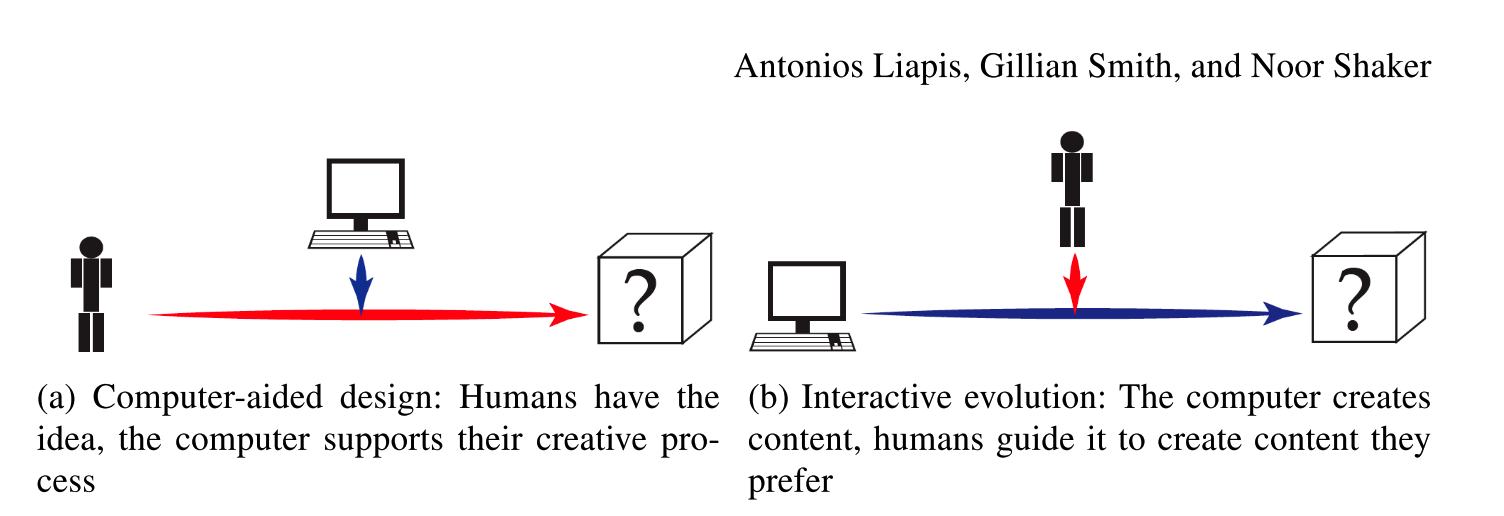
\includegraphics[width=1.0\linewidth]{figures/cadvsinteractiveevol.png}
    
    \caption[Two types of mixed-initiative design]{ Two types of mixed-initiative design, taken from \cite{Liapis2016} %
      \label{fig:mixedinitiativeimg}}
\end{figure}

Mixed-initiative systems have been used for generating various components in games. We are aware of the Sentient Sketchbook for strategy game map generation \cite{Liapis2013}, the Tanagra system for 2d platformer designs  \cite{Smith2011} and the dungeon creation system from \cite{Baldwin2017}.

Furthermore, for puzzle games in specific, M. Shaker et al. created a mixed-initiative system called Ropossum used for creating Cut The Rope levels \cite{Shaker2013} \& \cite{Shaker2013Ropossum}, in which they pioneered such interactive tools for physics-based puzzle games. Similarly to the automatic approaches, they also distinguish between the generator, the solver, and the curator, with the difference that the generator uses a Grammar Evolution technique that prompts the user to guide it.

Additionally, \cite{Butler2013} made a mixed-initiative system for Refraction, which is a puzzle game that lends itself well to a logical formulation. In their system, they were able to formulate some concepts that the player should learn in order to solve a level. From there, their tool generates progressions of levels that contain more and more of these concepts. The mixed-initiative aspect involved tweaking this progression by letting the user choose which concepts should appear in which level of the progression.

All of these mixed-initiative tools target a very specific set of problems, which make their methods hard to generalize for other games.

This has also been noticed by \cite{MacHado2018}, who also mentions all these mixed-initiative systems. They complain about a \textit{lack of generalisability} in current results and a \textit{lack of empirical justification} mentioning that there is a dearth of literature on the human factors of mixed-initiatives systems designed for game development tasks, something we try to address in this study.

To address \textit{lack of generalizability} they have created the game description language VGDL. 
On top of it the created Cicero, a tool that supports the following key features: agent-based testing for automatic gameplay testing, replay analysis for storing and playing back gameplay sessions, playtrace aggregation to visualize where players and agents tend to move on the game map and a mechanics recommender which retrieves mechanics from a large variety of games and Kwiri which is a tool to analyze why certain actions happen which is useful for debugging moves. 
Another one of these larger frameworks is \cite{Osborn2011} who has created the language \textit{Gamelan} inspired by board game rules, for modeling, among others, card games like Dominion. Also, \textit{BIPED} was yet another mixed-initiative system developed by \cite{Smith2008} for creating prototypes more quickly. Both of these frameworks have to our knowledge unfortunately not been used outside of their respective study.
In the end, I think we singled out a good balance of generality by focusing on grid-based puzzle games with agents.

Regarding \textit{lack of empirical justification} for using such tools to our knowledge only the recent work by \cite{Guzdial} has done a think-aloud user-study on their mixed-initiative system \textit{Morai maker} for creating Super Mario Bros. levels. We will highlight shared insights in our study. % regarding the adaption of the designers towards the system and regarding concerns about the use of such tools.
 Their study was carried out from a sample of students of which only a small subgroup has designed game levels before, whereas our study is exclusively done with people who have spent a considerable amount of time with puzzle game design. They mentioned that Morai Maker was either used as an unintentional inspiration source or an intentional means of getting over a lack of ideas.

\cite{Nelson2009} gathered a requirement analysis of video game design tools. He mentions Sutherland's claim of: \say{it is only worthwhile to make drawings on the computer if you get something more out of the drawing than just a drawing}, a claim we hope to make about this tool as well. They continue to mention \cite{Lawson1997}'s five roles for a mixed-initiative system in the design conversation: learner, informer, critic, collaborator, and initiator. In this study, we mostly focus on the aspects of informing, criticizing, and collaborating, although all five aspects are present in one form or the other.

Furthermore, \cite{Nelson2009} mention the term \textit{window dressing} which is the act of removing redundant solution paths and the distinction between  \textit{operational mechanics} and \textit{constitutive mechanics}. They also mention the lack of a design vocabulary and that having one would make further research clearer and more approachable. For this reason, we try to frame our results in their terms. Finally, they also address \cite{Giaccardi2008} suggestion that tools ought to support \textit{problem framing} as well as \textit{problem solving}. This is in line with the research on \textit{creative constraints} that suggest that limiting the possibilities can minder the \textit{paralysis of choice}. We will see concrete ways on how designers constrain themselves and how our tool help constraining them in the fifth chapter.

\chapter{MixedAim: The Mixed-Initiative System}

\section{PuzzleScript}

The programming language with which designers can implement puzzle games in MixedAim is \href{https://www.puzzlescript.net}{PuzzleScript}\footnote{https://www.puzzlescript.net @ PuzzleScript} developed by Stephen Lavelle (also known as increpare).
In the appendix \ref{fig:sokobaninpuzzlescript}, you can see a full Sokoban implementation in PuzzleScript for reference.

PuzzleScript is grid-based, and each PuzzleScript game consists out of the following seven sections.
\begin{description}
    \item[Objects] In here, the objects of the grid and their style are declared. For Sokoban, you would have to declare the following objects \textit{Background, Walls, Player, Crate, Target}. \textit{Player} and \textit{Background} are special objects and always need to be declared. \hfill
        \begin{figure}[!htbp]
    \begin{minipage}{0.4\textwidth}
        \centering
    \begin{lstlisting}
========
OBJECTS
========
Wall
BROWN DARKBROWN
00010
11111
01000
11111
00010
    \end{lstlisting}
    
    \end{minipage} \qquad $\Longrightarrow$ \hfill
    \begin{minipage}{0.4\textwidth}
        
        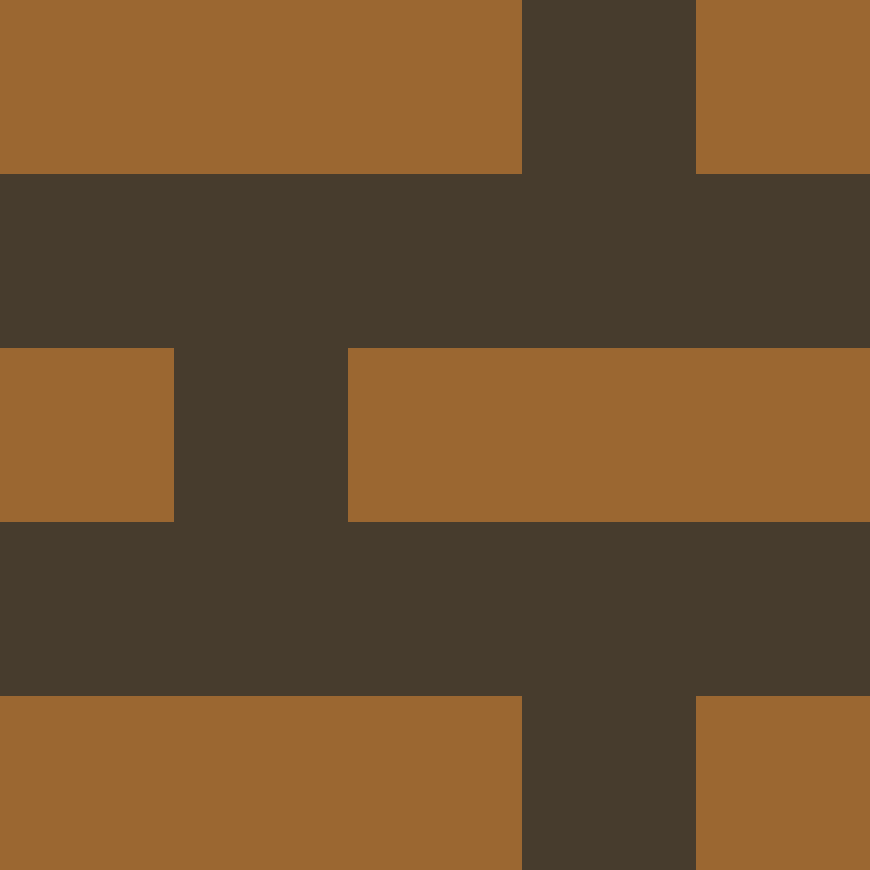
\includegraphics[width=0.55\textwidth]{figures/wallimg.png}
    \end{minipage}
    \caption{Objects section}
    \end{figure}



    \item[Legend] In the legend,  three kinds of names can be specified.
        \begin{enumerate}
            \item Define a synonym for an object. \hfill \\
            Example: \lstinline{# = Background}
            \item Define an aggregate, which is a symbol for referencing a tile that includes multiple objects. It is not possible to create an aggregate from objects which belong to the same collision layer. \hfill \\
            Example: \lstinline{@ = Target and Background}
            \item Define a property, which references any tile that contains any of the objects included in its definition. \hfill \\
            Example: \lstinline{Obstacle = Wall or Crate or Player or Target}.
        \end{enumerate}
        
        It is worth mentioning that you cannot make aggregates from properties or vice-versa.
    
    
    \item[Sounds] can be used to add chip-tunes generated with \href{https://www.bfxr.net}{Bfxr} \footnote{https://www.bfxr.net}.
    
    \item[Collisionlayers] define on which layer which objects are stored. In PuzzleScript a level is rendered by multiple two-dimensional layers layered on top of each other.
     In this way you can specify that both a \textit{Player} and a \textit{Wall} cannot both occupy the same tile while a \textit{Crate} and a \textit{Target} can.
     
             \begin{figure}[!htbp]
    \begin{minipage}{0.4\textwidth}
        \centering
    \begin{lstlisting}
================
COLLISIONLAYERS
================
Background
Target
Player"Wall"Crate
    \end{lstlisting}
    
    \end{minipage} \qquad $\Longrightarrow$ \hfill
    \begin{minipage}{0.45\textwidth}
    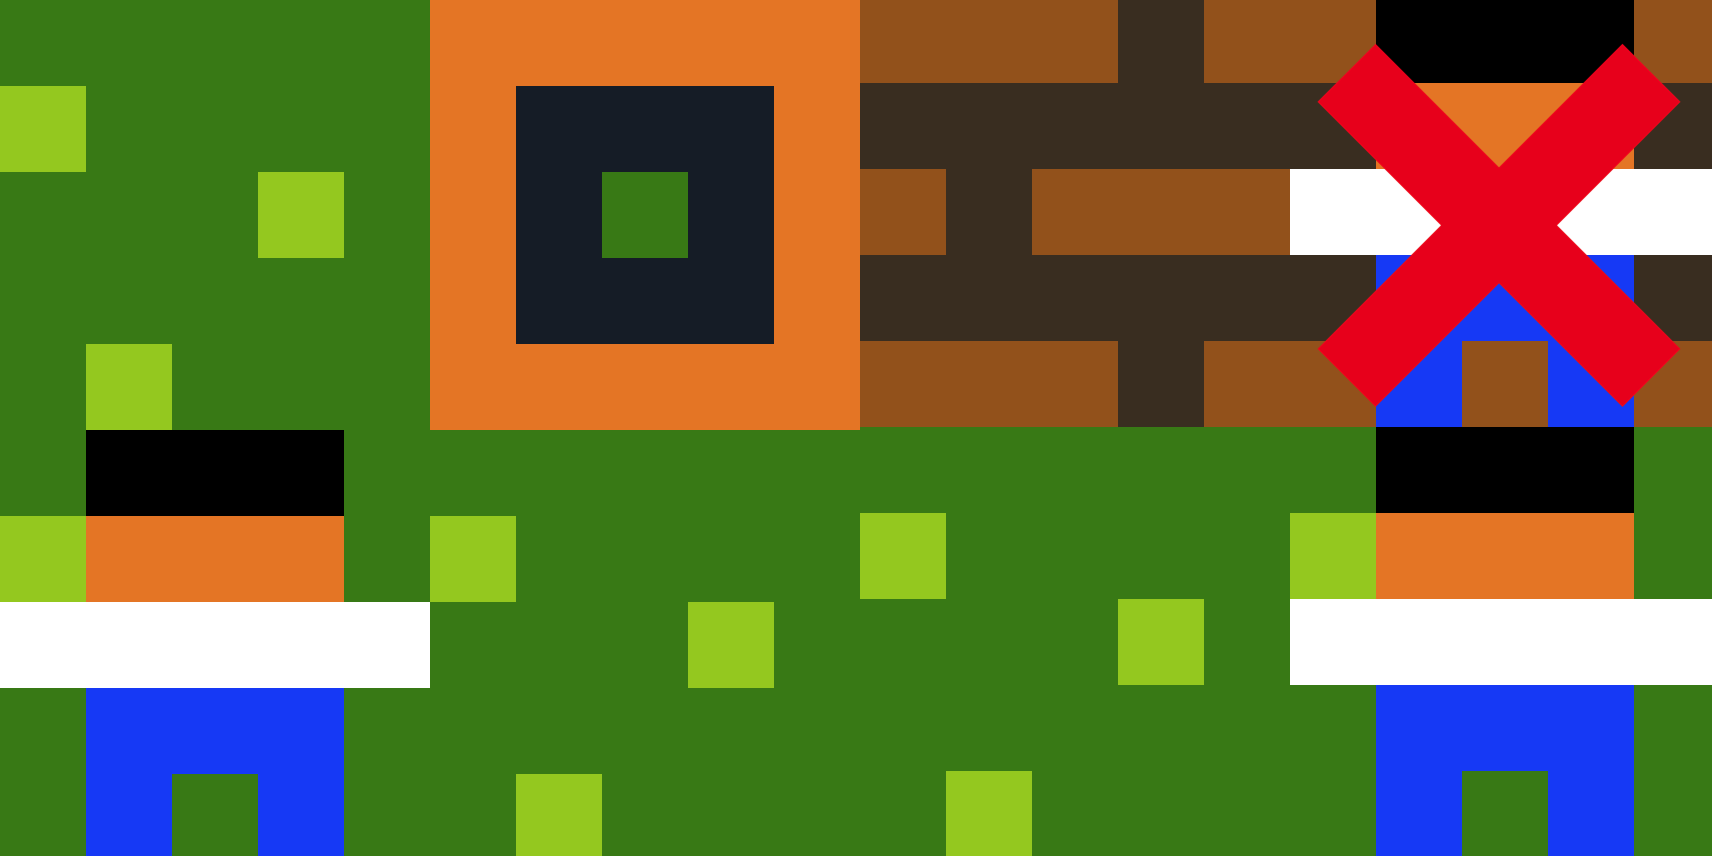
\includegraphics[width=0.7\textwidth]{figures/collisionlayersboth.png}
    \end{minipage}
    \caption{Collisionlayers section}
    \end{figure}
    
    \item[Rules] The rules are deceptively simple and are structured in the following form \: \lstinline{Match -> Replace}. \textit{Match} consists of either rows or columns that have to be matched and \textit{Replace} must be of the same size stating with what the objects will be replaced.
        
        In case you are wondering how inputs are handled, you have to know that every object can come with force attached to it (highlighted in green by the examples).
        When the player presses the right button, all \textit{Player} objects get the right force assigned to them. In the end, when all (non-late) rules have been applied, each object will try to move in the direction of their force. This will succeed provided there is no object of the same collision layer in that direction.
        
        The rules of Sokoban can be written with a single rule: \hfill \\
        \lstinline{[> Player | Crate] -> [ > Player | > Crate ]}
        
        This rule is implicitly expanded in 4 directions, so it works both on columns and rows:\hfill \\
        \lstinline{RIGHT  [right Player | Crate] -> [right Player | right Crate]}\hfill \\
        \lstinline{+ UP   [up    Player | Crate] -> [up    Player | up    Crate]}\hfill \\
        \lstinline{+ DOWN [down  Player | Crate] -> [down  Player | down  Crate]}\hfill \\
        \lstinline{+ LEFT [left  Player | Crate] -> [left  Player | left  Crate]}\hfill \\
        
        To match multiple rows/columns at once, you can use multiple boxes. Take the following rule as an example. If the player is on top of a key and there is a door on the map, then remove the key and the door.
    \lstinline{[Player Key] [Door] -> [Player] []}
    
        Lastly, every command can execute \textit{commands} if the rule is executed, such as playing a tune defined in sounds, stopping the current moves (\textit{cancel}), replaying the rules another time (\textit{again}) \& more.
        
        Additionally, you can use properties and aggregates when rule building, use the keyword \textit{No} to make sure no object/aggregate/property matches, use an ellipsis for arbitrary distances, build groups of rules, make these groups rigid \& a lot more.
        
        For more details please consult the \href{https://www.puzzlescript.net}{PuzzleScript}\footnote{https://www.puzzlescript.net @ PuzzleScript} manual.
        
        We also linked a BNF grammar for a single syntactically correct PuzzleScript rule (without rule grouping) \ref{fig:puzzlescriptrulebnf}.
    
    \item [Winconditions] In this section, you can add multiple win-conditions which all need to be satisfied in the level state simultaneously to `win' a level.
    
    The rules can be any of the following: \textit{No X, Some X, No X on Y, Some X on Y, All X on Y} where X and Y can be objects or properties and do what you would expect them to do.
    
    \item[Levels] is the section where you can specify the puzzle problems, also referred to as levels.
    The previously defined objects/synonyms/aggregates with a single letter can be used to create the level.
            \begin{figure}[!htbp]
    \begin{minipage}{0.4\textwidth}
        \centering
    \begin{lstlisting}
========
LEVELS
========
####..
#.O#..
#..###
#@P..#
#..*.#
#..###
####..
    \end{lstlisting}
    
    \end{minipage} \qquad $\Longrightarrow$ \hfill
    \begin{minipage}{0.4\textwidth}
        
        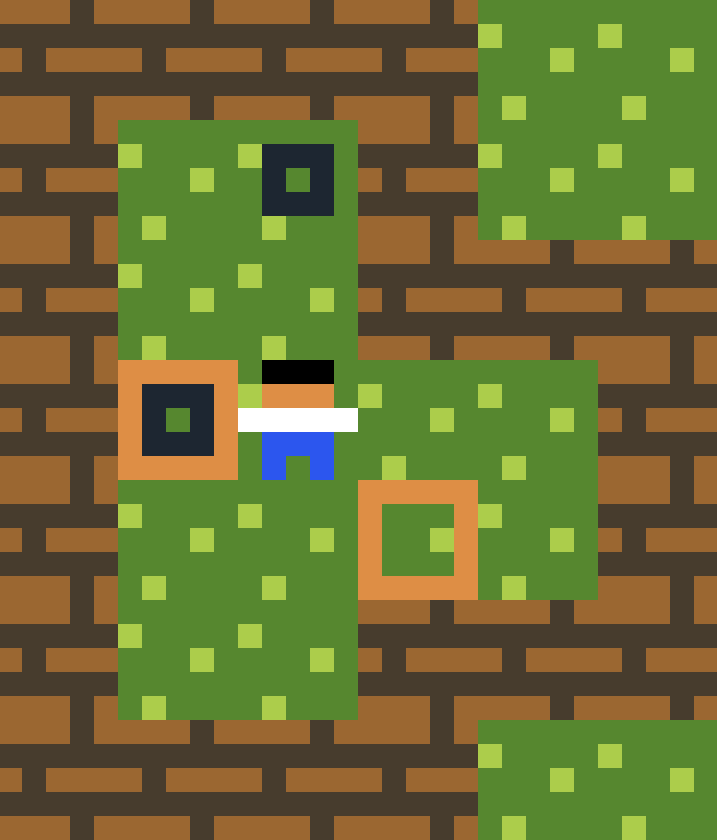
\includegraphics[width=0.55\textwidth]{figures/level1.png}
    \end{minipage}
    \caption{Levels section}
    \end{figure}
     
\end{description}


\section{User interface}

The mixed-initiative system we developed to create PuzzleScript levels is comprised of three modes of operation: The \textit{level editor mode}, where the designer can place the blocks on the level, the \textit{playtest mode}, where the player can test the level and see if it is solvable from a certain position and lastly the \textit{transform mode}, where the designers can steer the passive suggestions which are shown both in the \textit{level editor} and in the \textit{transform mode}.

%   a level they are working on in order to see possible variations of the design and get inspired by them.

% \cite{Lawson1997} roles for the mixed initiative system are as follows.
\begin{figure}
\centering
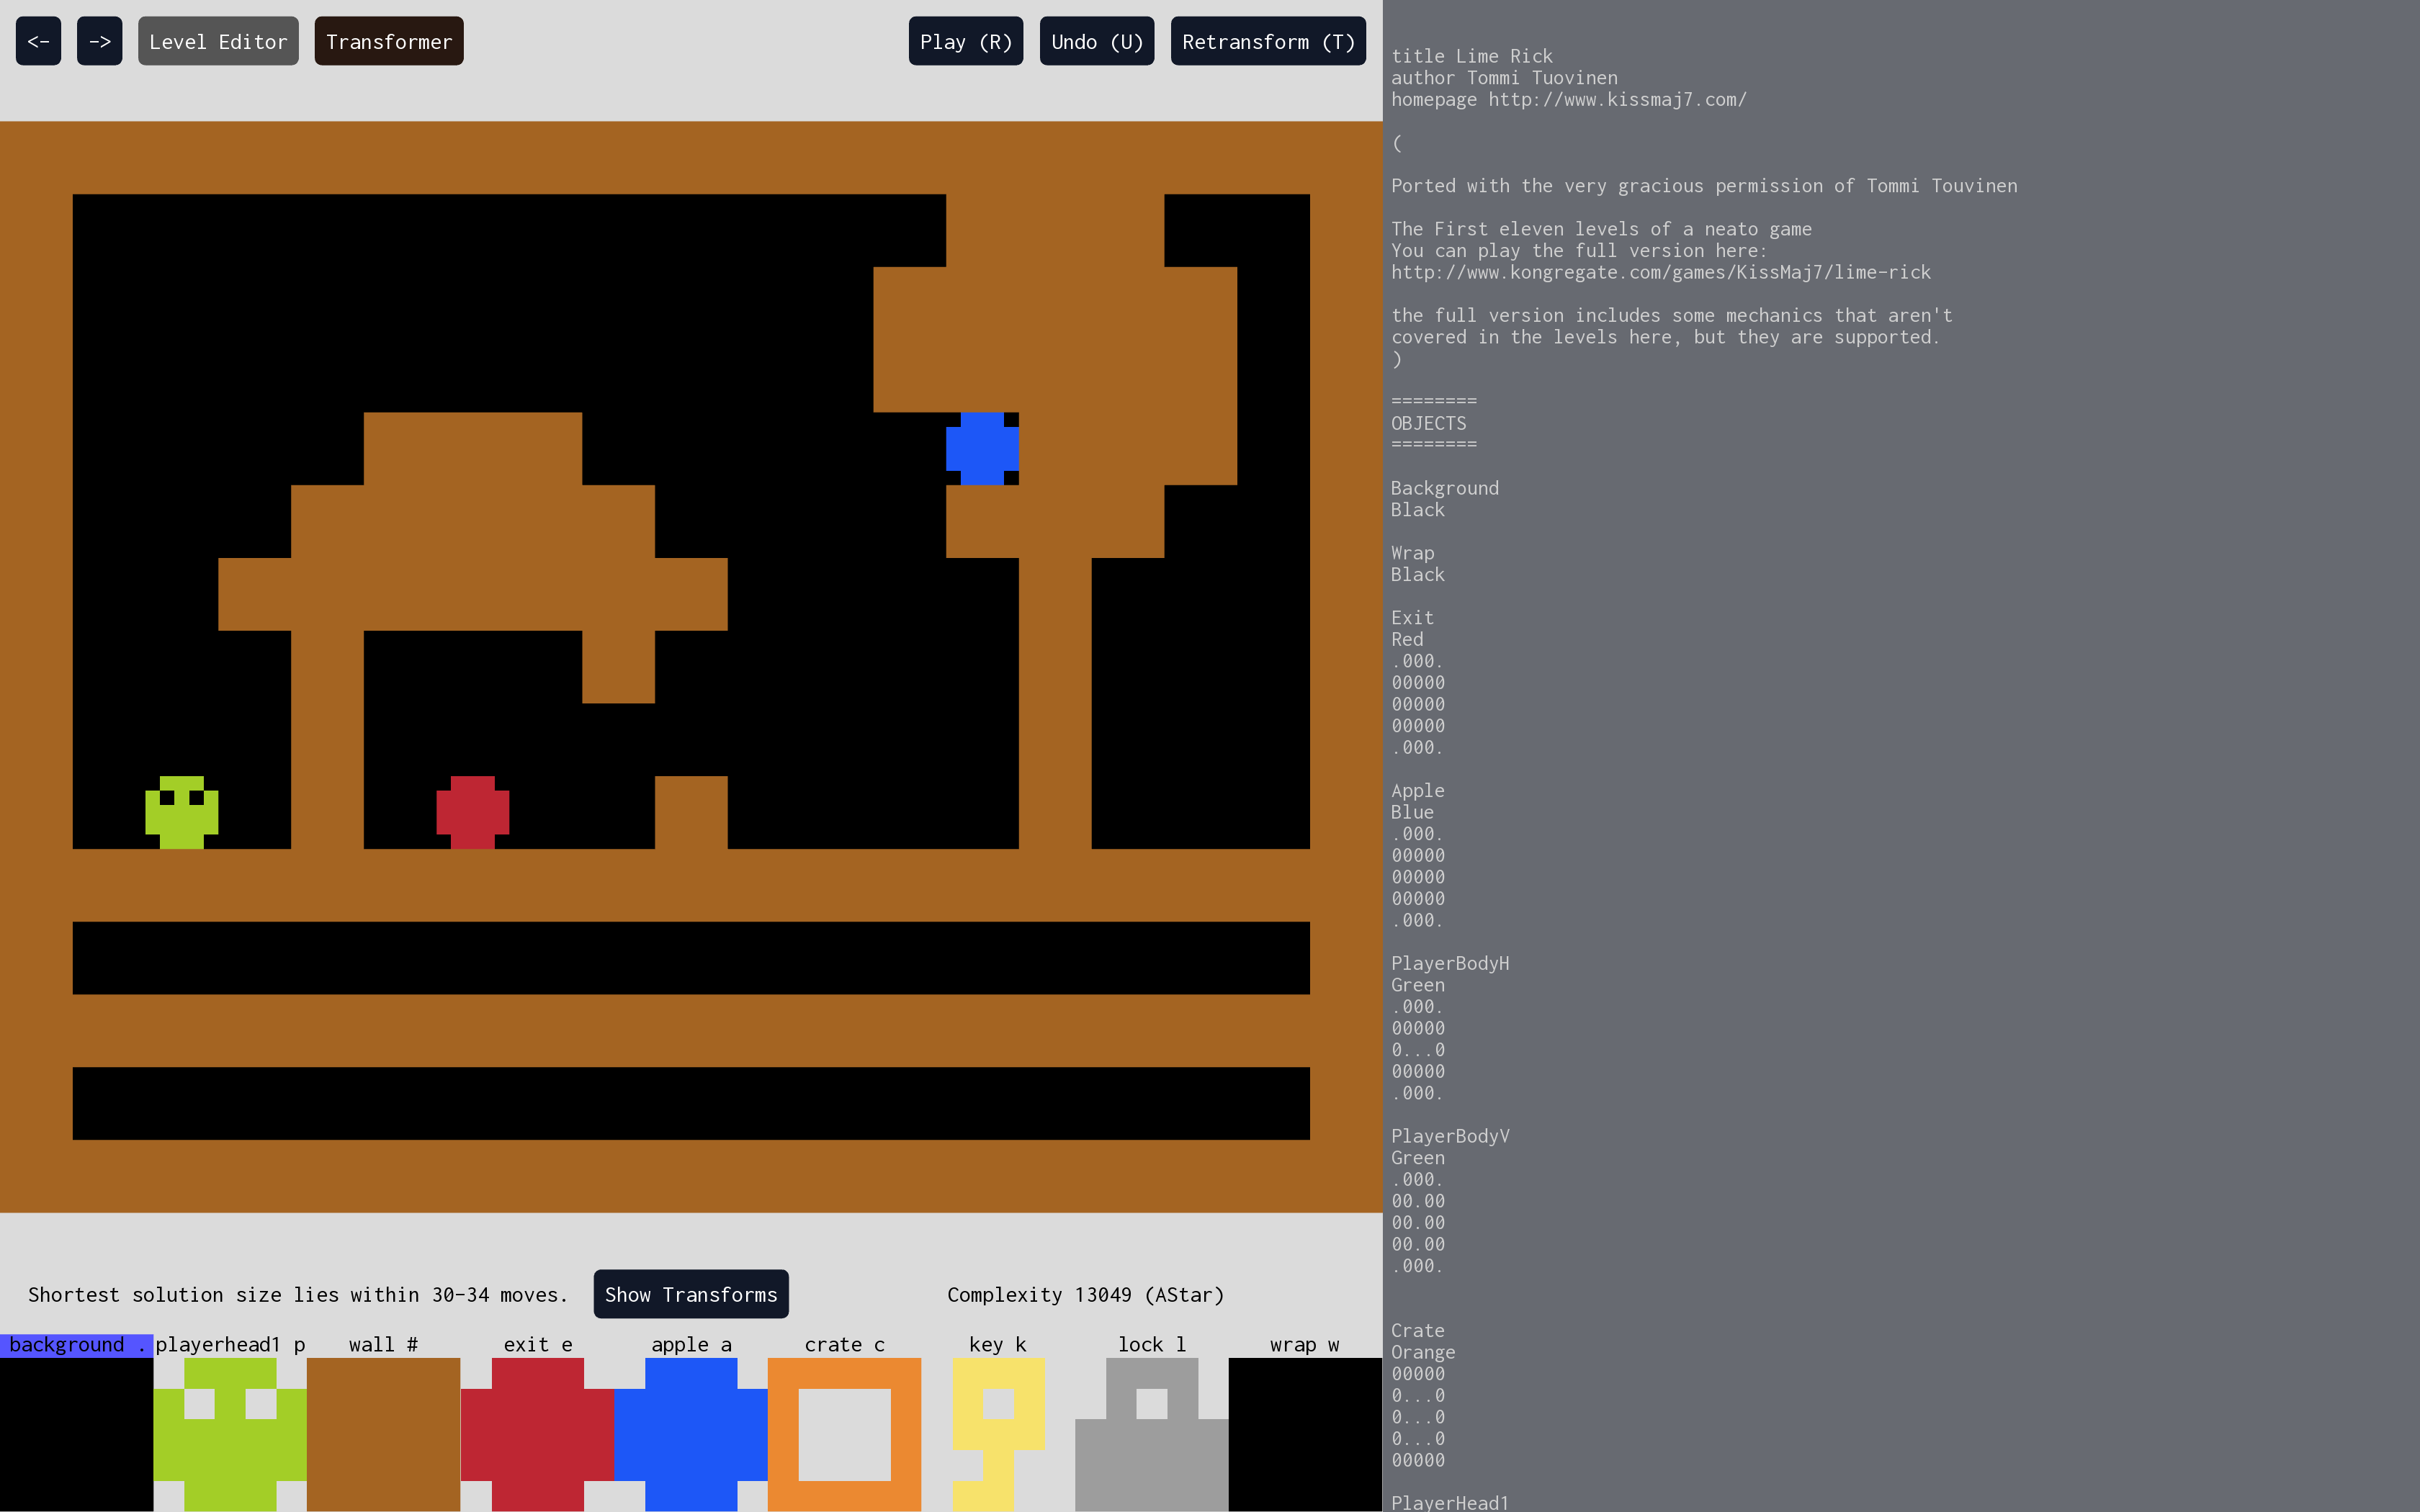
\includegraphics[width=1.0\linewidth]{figures/leveleditormode.png}
\caption[LevelEditor]{Level Editor Mode\label{fig:leveleditormode}}
\end{figure}


\begin{figure}
\centering
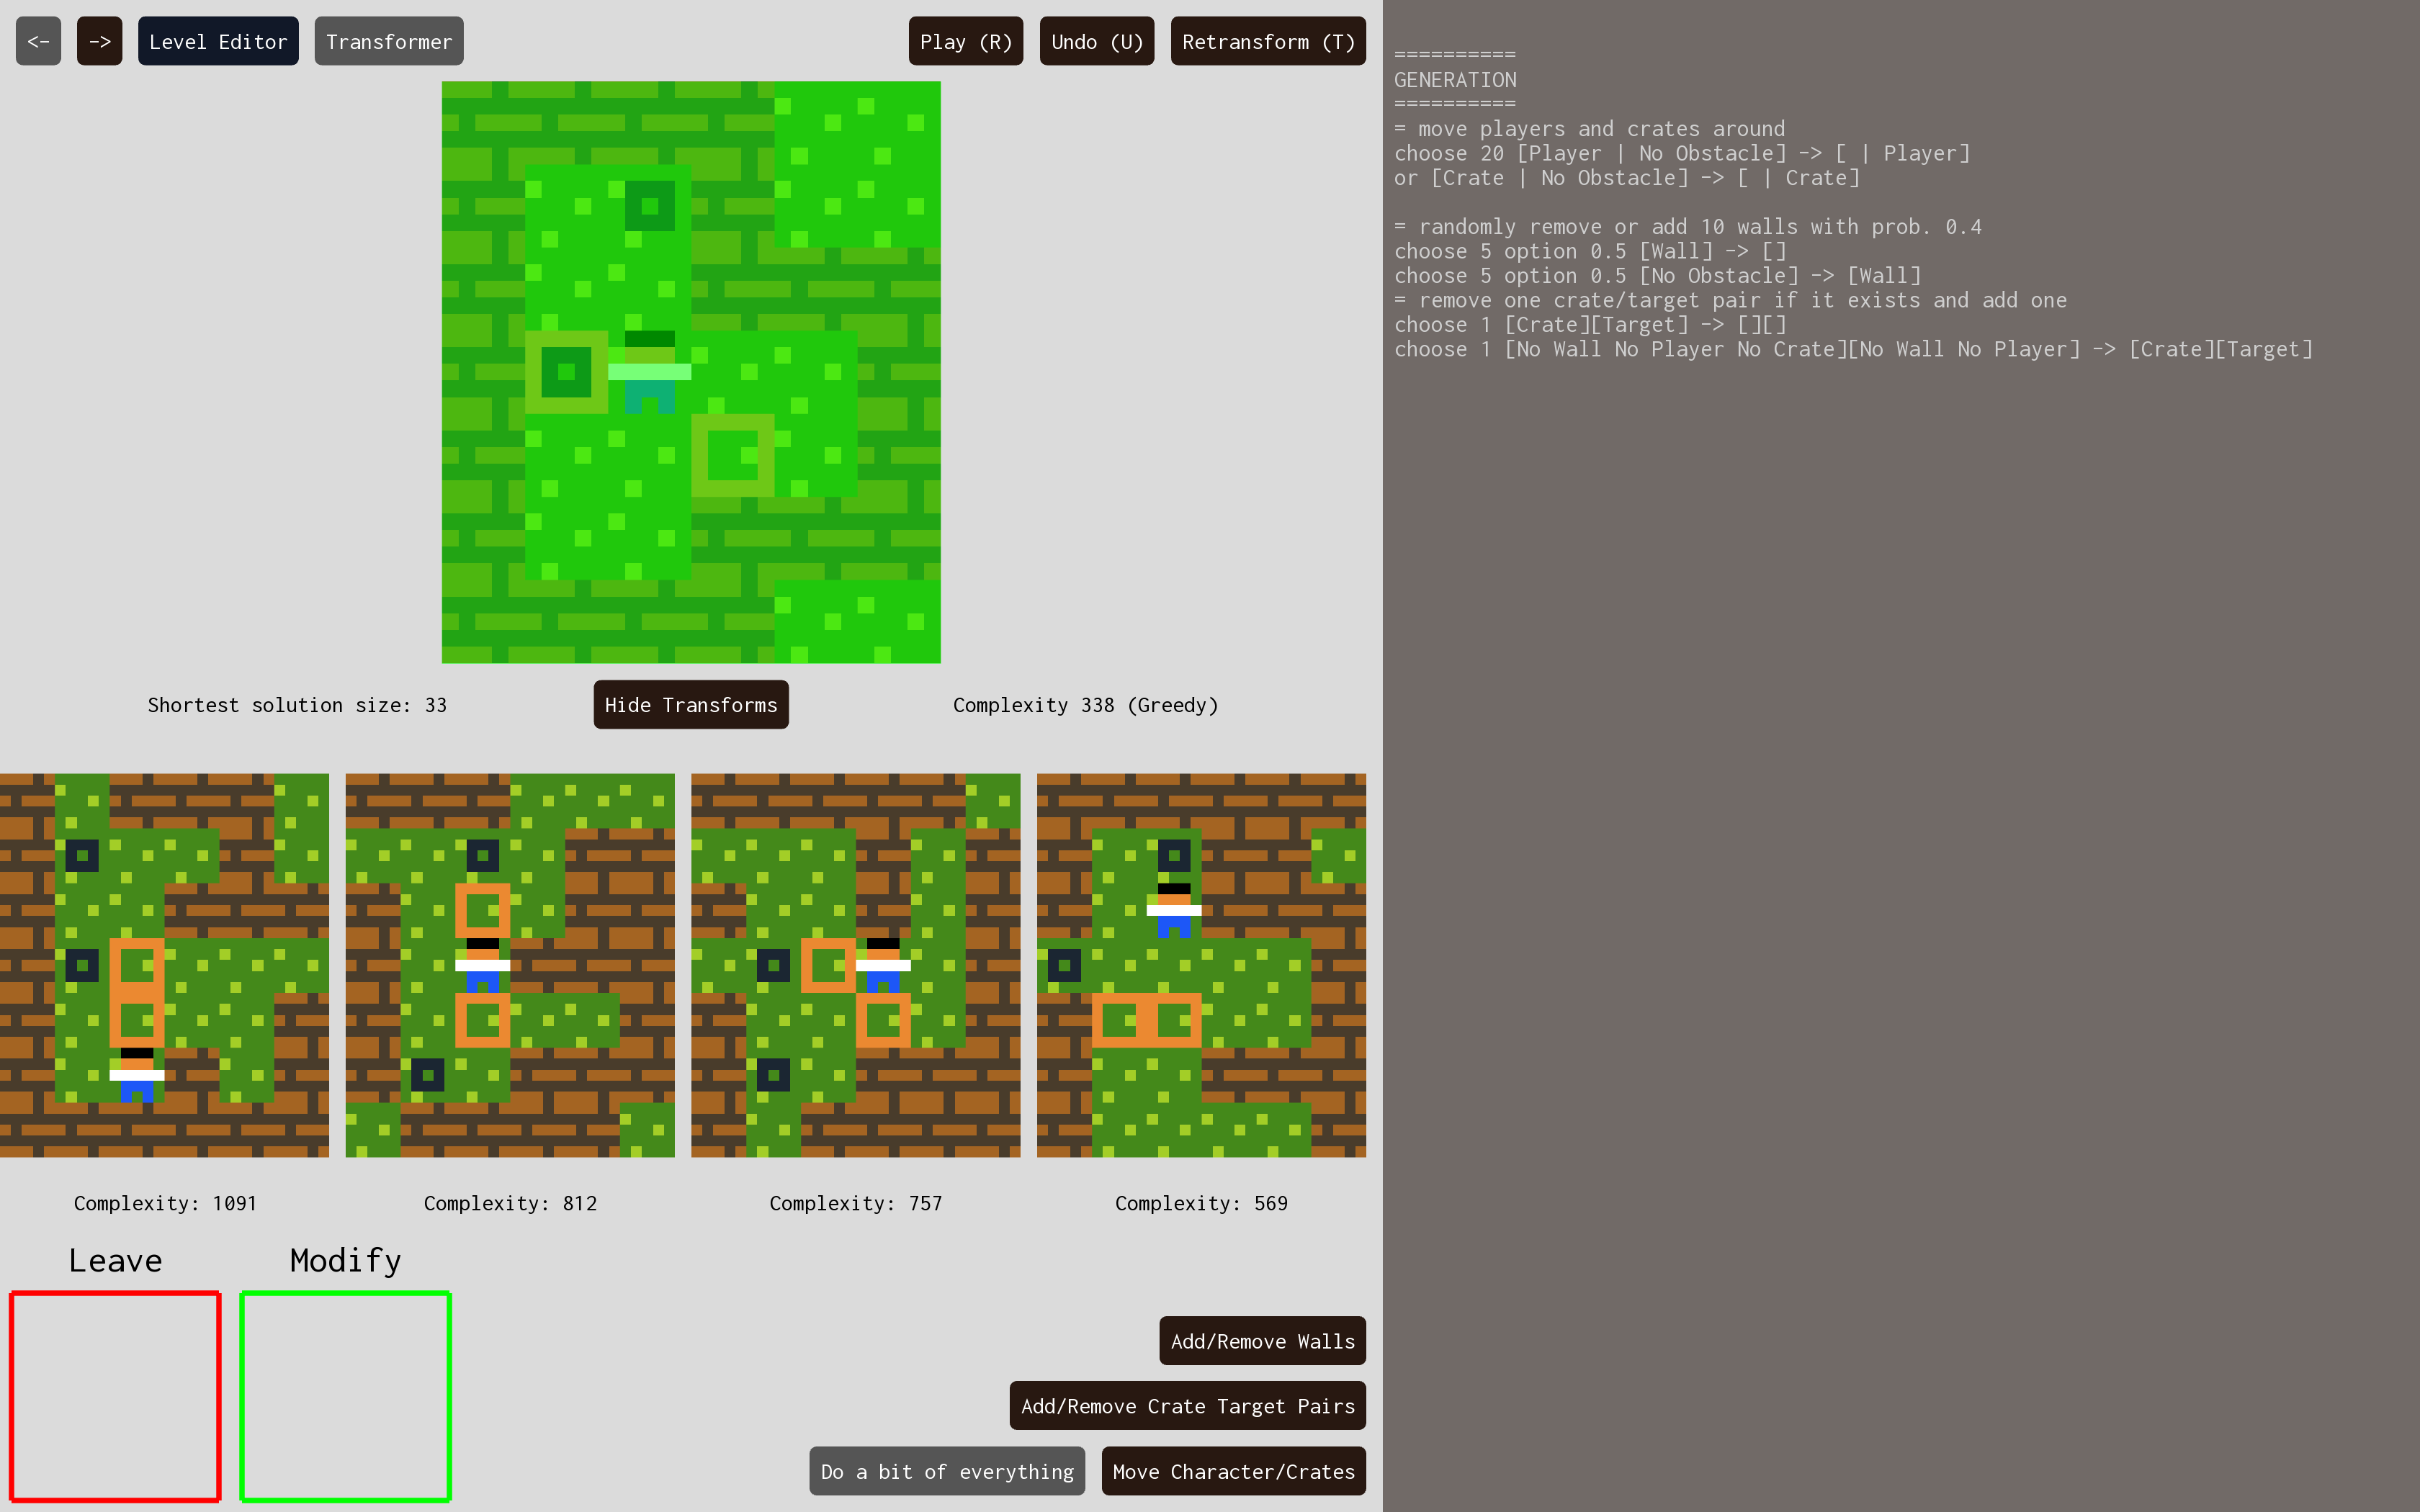
\includegraphics[width=1.0\linewidth]{figures/imageoftransformmode.png}
\caption[Transformer]{Transform Mode\label{fig:transformermode}}
\end{figure}


\begin{figure}
\centering
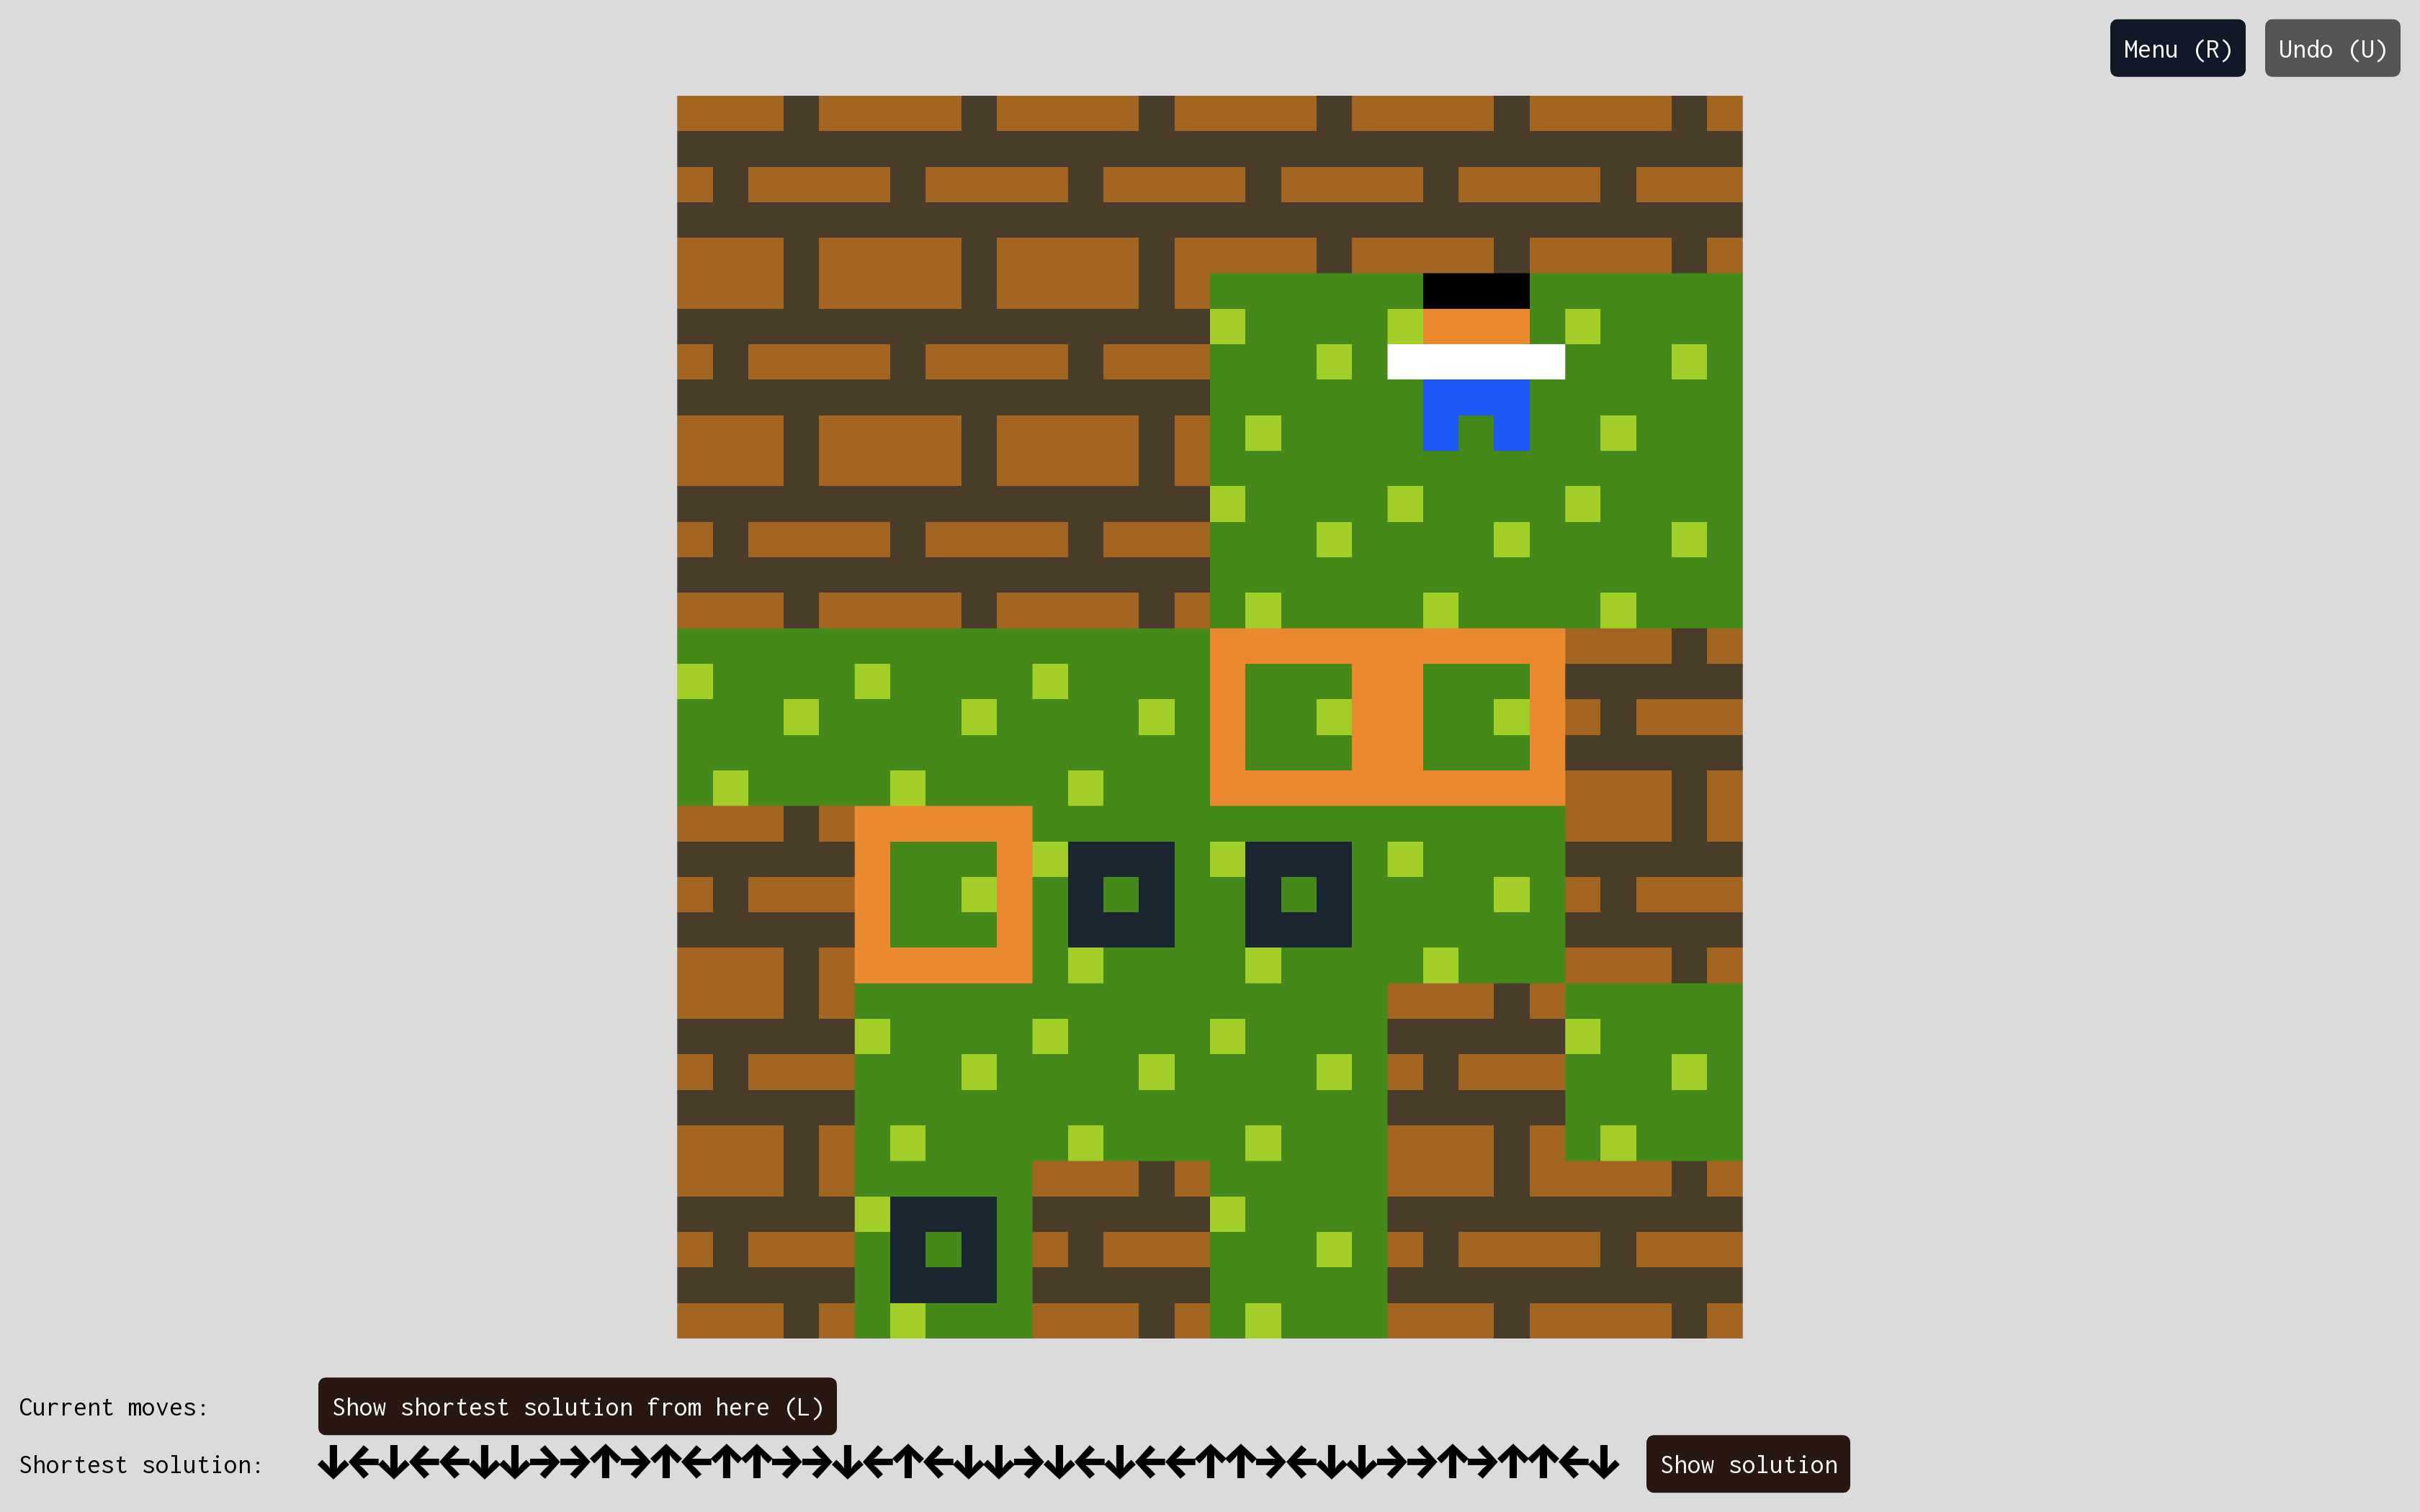
\includegraphics[width=1.0\linewidth]{figures/playtestmode.png}
\caption[Playtest]{Playtest Mode\label{fig:playtestmode}}
\end{figure}

Information about the current level is passively shown at all times to the designer [\ref{fig:passiveinformation}] and includes information like whether or not a level is solvable and, if it is, in how many steps at least. Additionally, it also displays the difficulty of the level.
This allows designers to quickly see whether a modification on a level they are working on is still solvable without needing to solve it themselves. In the next chapter, we will discuss in which ways designers exploit this when designing a level.


\begin{figure}
\centering
\hfill
\begin{minipage}[t][5cm][b]{0.35\textwidth}
\centering

\includegraphics[width=1.0\linewidth]{figures/shortestsolution.png} \hfill

\includegraphics[width=1.0\linewidth]{figures/shortestsolutionwithin.png}\hfill

\includegraphics[width=1.0\linewidth]{figures/nosolutionwithin.png}\hfill
Solve Information
\label{fig:solveinformation}
%\caption{Solve \\ Information}
\end{minipage}
\begin{minipage}[t][5cm][b]{0.25\textwidth}
\centering

\includegraphics[width=1.0\linewidth]{figures/difficultygreedy.png}\hfill

\includegraphics[width=1.0\linewidth]{figures/difficultyastar.png}\hfill

\includegraphics[width=1.0\linewidth]{figures/difficultybfs.png}\hfill
\label{fig:solveinformation}
Difficulty Information
%\caption{Difficulty Information}
\end{minipage}
\begin{minipage}[t][5cm][b]{0.35\textwidth}
\centering

\includegraphics[width=1.0\linewidth]{figures/difficultycurveleft.png} \hfill

\includegraphics[width=1.0\linewidth]{figures/difficultycurveright.png}\hfill
\label{fig:solveinformation}
Greedy vs. AStar vs. BFS
%\caption{Greedy vs. AStar vs. BFS}
\end{minipage}


\caption{Passive information displayed to the user\label{fig:passiveinformation}}
\end{figure}


\section{Solver \& Difficulty}
To check solvability, we employ three different types of solver: Breadth-first search, A* search, and Greedy best-first search.

Both A* and Greedy search need a heuristic which, given a state, approximates the number of steps the state is away from a solution. Ideally, this heuristic never overestimates the number of steps, making it admissible \ref{eq:admissibility}.

It is well-known that A* performs optimally (finds the shortest path) on average in the sense that it has to explore the least number of states given such a heuristic and assuming no additional domain knowledge is used during the search.

\begin{equation}
\label{eq:admissibility}
\forall s_i \in \text{STATES} \: . \: h(s_i) \leq \text{min-cost-to-goal-from}(s_i)
\end{equation}
    
However, a very common additional domain knowledge is to store which states have already been visited (referred to as closed states). In a lot of puzzle games, like Sokoban, it is possible to end up in the same state via multiple paths. For example, moving up or moving left, up, right leads to the same state if no obstacles block the path. If the heuristic function is monotone/consistent \ref{eq:monotone} then A* remains optimal without having to recompute already visited states. Notice that not all puzzles profit from this, trapdoor puzzles or puzzles where one moves an ever-expanding snake for example, in which case storing closed states is just a small overhead. 
    
\begin{equation}
\label{eq:monotone}
\forall n_i \in \text{NEIGHBOR}(s_i) \: . \: h(s_i) \leq d(s_i, n_i) + h(n_i)
\end{equation}

We do not necessarily care about the optimal solution (shortest in terms of moves) though and care more about whether or not a solution exists. 

Thus regardless of whether or not our admissible heuristic function is monotone, re-searching already visited states (states in the closed list) would only add more states to explore. While it might in a few cases be better to re-search these nodes in some cases with the new value, we decided not to do that.

In practice, the greedy best-first search outperforms A* in a lot of cases and BFS in some other cases (tested games include Sokoban, LimeRick, Sokobond). When Greedy performs better than A*, then usually BFS performs even worse and when BFS performs better than A* then usually Greedy performs even worse (we were not able to find a pre-crafted level of Sokoban, LimeRick or Sokobond where this was not the case).


The heuristic we use for the A* and Greedy solver is a generalized version of \cite{Junghanns1999} Sokoban heuristic. Since every crate has to be pushed on a target (and two crates cannot be on the same target) Junghanns observes that the minimal matching between crates and targets is an admissible heuristic for the number of pushes remaining (rounded down).

The win-condition of Sokoban implemented in PuzzleScript is: \lstinline{All Crate on Target}. Notice that there can be more targets than crates, so we want to find the minimal-cost maximum matching.

\hspace{\dimexpr-\fboxrule-\fboxsep\relax}\fbox{%
  \begin{minipage}[t]{\textwidth}
A PuzzleScript file can contain multiple win-conditions that all need to be satisfied. We compute the heuristic $h(s)$ for state $s$ as the sum of all of the following win-conditions:  \hfill      \begin{description}
\item[No X:] As soon as X is nowhere on the level state this win-condition is triggered. We add +1 cost for every X appearing on the state s.
\item[Some X:] As soon as X is somewhere on the level state this win-condition is triggered. We add +1 cost if no X is found in the state s.    

\item[No X on Y:] We add +1 for every tile that has both X and Y on it.
\item[Some X on Y:] We compute the closest X,Y pair in terms of their Manhattan distance and add their distance towards the cost function.
\item[All X on Y:] We compute the minimal-cost maximum matching on the Manhattan distance of all $X,Y$. Although such matchings can be computed in polynomial time, computing these still bring a large overhead. Instead of using this, we use a maximal matching, which is a matching obtained by greedily taking the $X,Y$ pair with smallest Manhattan distance. It is well-known that a minimum cost perfect maximal matching is at worst twice as large as a minimum cost maximum matching. For this reason, we compute the cost of a maximal matching and divide the cost by 2. In this way, the heuristic will not overestimate the cost.
\end{description}
\end{minipage}%
}

Notice that this heuristic is not always admissible depending on the rules. This is not a problem in most cases. For example, in Sokobond, a game where you need to connect atoms until all electrons have bonded, the win condition is \textit{No Orbitals}. In this game, it is possible to bond multiple orbitals with a single move. The heuristic only ever overestimates the solution by a constant factor of at most 3 (since you can connect up to 4 atoms with a single move).

The \textit{difficulty} of a level depends on the solver and is subjective. We define difficulty to be the number of (open) states the solver has to explore to find the solution.

We expect that a level which is easy to solve for a solver also tends to be easily solved by human players. Thus our difficulty metric is simply the minimum complexity of all solvers.

\lstinline{difficulty := min(diff(Greedy), diff(AStar), diff(BFS))}

Ideally, designers should gauge the difficulty themselves wherever possible since difficulty between human players is still more predictable.

This approach is not the only approach to approximate difficulty. \cite{Science1996} gauged the difficulty of Sokoban levels through a combination of the parameters: length of solution, number of changes in directions of pushing of minimal solution \& number of detours in a solution sequence. In the suggestions, we mention a way in which designers could choose their own curation criteria for their puzzle game.

% For future work it would be interesting to see how designers would write  such difficulty measures. One thing we want to try out in the future is to add cost to rules: \lstinline{[ > Player | Crate ] -> [ > Player | > Crate ] COST 10}. This way, a solution that contains a lot of block-pushes costs more and hence makes levels with higher cost more sensitive.

Another interesting idea comes from \cite{Pelanek2011}, \cite{Jaru}, who noticed that most Sokoban levels have a bottleneck. It is possible to look at the graph of all possible paths leading to a solution and notice an hourglass shape. The value of this bottleneck is the maximum flow from the start to the goal state. Both easy and hard games tend to have this bottleneck, and computing its value is not feasible except for small examples. However, this made them model the human player as a solver moving uniformly at random until it comes within a certain distance of the goal, starting from which it will more accurately find its way towards the solution. Notice that these methods will not make solving the levels any easier but might give a more accurate result on the level difficulty if you can spend the resources. We decided not to implement this as finding a solution is significantly easier than constructing the graph of all possible paths let alone computing the maximum flow on it.
 
\section{Transformer}
The transformer allows the user to steer the passively shown suggestions by letting the user specify rules on what valid suggestions are.

We discovered a neat way of doing this which was to extend PuzzleScript with two simple commands \textit{choose} and \textit{option} making it non-deterministic: \\
\hspace{\dimexpr-\fboxrule-\fboxsep\relax}\fbox{%
\begin{minipage}{\textwidth}
\lstinline{option 0.4 [Wall] -> []} \hfill \\
will remove every wall with a probability of 0.4 \hfill \\

\lstinline{choose 5 [Wall] -> [Crate]} \hfill \\
will replace 5 walls chosen uniformly at random and replace them with crates. If there are less than 5 walls turn all of the walls into crates. \hfill \\

\lstinline{choose 5 option 0.4 [Wall] -> []} \hfill \\
will choose 5 walls uniformly at random and remove these with a probability of 0.4.

\end{minipage}
}

From these primitive rules, the designer can create more elaborate transformations. For the user-study we provided four such transformations: \textit{Moving Player/Crates, Add/Removing Walls, Removing/adding a target/crate pair} and finally \textit{`do a bit of everything'} which is a combination of the other three methods.

\begin{description}
    \item[Add/Removing Walls/Crates] \hfill \\
    Here we remove and add walls (on average we tend to add more walls instead of removing more walls as that seemed to provide better suggestions).
    \hfill \\
        
    \begin{lstlisting}
(randomly remove or add 20 walls with prob. 0.4)
choose 20 option 0.4 [Wall] -> []
or option 0.6 [No Obstacle] -> [Wall]
    \end{lstlisting}
        
    \item[Move Player/Crates] This preset moves around the crates and the player(s). Instead of using forces to move these objects, we can just use place/replace rules to move them around. In this way, the objects can be moved more than one tile.
    
       \begin{lstlisting}
(move players and crates around)
choose 20 [Player | No Obstacle] -> [ | Player]
or [Crate | No Obstacle] -> [ | Crate]  
    \end{lstlisting}         
    
    \item[Add/Remove a Crate/Target Pair]
    First tries to remove a crate/target pair in the modify section and then tries to remove it.

    \begin{figure}[!htbp]
    \centering
    \footnotesize
    \begin{lstlisting}
(remove one crate/target pair if it exists and add one)
choose 1 [Crate][Target] -> [][]
choose 1 [No Obstacle or Target][No Obstacle or Target] -> [Crate][Target]    
    \end{lstlisting}
    \end{figure}

\end{description}

\subsection{Suggestions} % Choosing difficult levels

The transformer specifies valid possible level suggestions. However, the tool cannot show all these possible suggestions and needs a way to display the best levels to the user automatically.
As mentioned in the introduction, we decided to use \textit{difficulty} as a discriminator and choose to passively show the four most difficult levels. More precisely, we use the notion of difficulty discussed in the previous section, namely, the minimum number of states any of the three solvers needs to explore before finding a solution.

Because solving a level takes time, we only ever use all three solvers on potential curated level candidates. We start by solving a level using only one solver and, if it turns out to be difficult enough to lie within the curated level candidates, we proceed by checking the difficulty with the other two solvers.

Additionally, we added a timeout to the solver, so from the point of view of the solver there are now three types of levels: Solvable levels, unsolvable levels, and levels on which the solver times-out before figuring out whether it is solvable or unsolvable.
This requires a careful timeout balance in order to not skip solvable but interesting levels and to not waste computational time on unsolvable levels which are difficult to prove unsolvable.
Initially, the timeout for each new level is set to a tenth of the time it already spent on trying to find a solvable level. As soon as a solvable level is found, the tool will always set the timeout threshold to 8 times the amount of time it took to solve the current curated levels. This method of increasing the threshold leads to a quick succession of freshly curated levels at the start, which slows down as it gets proportionally harder to find more difficult levels.


\chapter{User Study and Results}

We did two user-studies: One need-finding survey, which we discussed in the introduction, and one study to evaluate MixedAim based on a think-aloud session followed by a structured interview. 

Both user-studies are qualitative rather than quantitative and have the purpose of informing, i.e., obtaining interesting research questions and finding interactions that provide `genuine value' to the designer. 

Quantitative studies are usually carried out on `tried-and-tested' design approaches and serve to test a hypothesis or to compare the effectiveness of one approach towards other approaches.
Due to the scale of the project and the dearth of similar tools, we decided that a qualitative study, specifically the think-aloud session, would provide more insights into the design of mixed-initiative systems for puzzle games. In hindsight, this turned out to be a good decision as our users found new ways of using the tool which we did not anticipate.
While we did gather clickstream data, due to the different ways that users approached the tool, we were not able to draw meaningful conclusions from it. 

This second user-study had 7 participants, 6 of which are very experienced puzzle game designers (with a median experience of 3 years). The remaining participant is an experienced game designer (5 years of experience outside of puzzle games). For more details on the participants, see \ref{tab:demography}.

The user-study was carried out remotely via a video call and a screen capture of the participants' machine except for participant 6, who did the same user-study process but on our machine. The outline of the study looked as follows:

\begin{enumerate}
\item  First, we asked the participants some questions related to their experience as a (puzzle) game designer (see \ref{tab:demography}).
\item Second, we asked the participants to design one or more Sokoban-levels for ~60 minutes and asked them to think-aloud their thoughts during the design process.
\item Third, we optionally gave the participant time to explore the tool further and use their PuzzleScript games to design levels. In particular, participant 1 \& 4 have worked multiple days with the tool and have found interesting use-cases which we did not anticipate before proceeding with the final interview.
\item Lastly, we concluded with a structured interview.
\end{enumerate}


\section{Think-aloud study results}
For the think-aloud study, we asked participants to design one or more Sokoban-levels. 
Since we are interested in seeing whether mixed-initiative systems can help designers iterate upon their design, we suggested to try turning the following Sokoban level \ref{fig:sokobaniterate} into a more difficult level. Some designers then used our mixed-initiative system exactly the way we anticipated, while some other participants found other surprising ways of utilizing the tool. For this reason, we decided to divide this section into the different styles in which the participants used the tool to design levels.


\begin{figure}
\centering
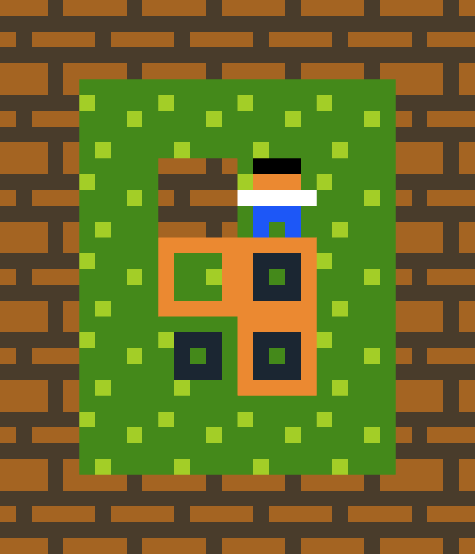
\includegraphics[width=0.5\linewidth]{figures/sokobaniteratelevel.png}
\caption[SokobanIterate]{Sokoban level participants were prompted to iterate upon\label{fig:sokobaniterate}}
\end{figure}

% Interestingly, not all designers we interviewed followed (or even attempted) to use the iterative design method. We believe this might be because these designers either tried to fit their own method onto the tool (with varying degrees of success) or started to simply play around with the tool to exploit all the possible ways of creating levels.


\subsection{Iterative design}

The iterative design approach was the primary way we intended users to design levels. We encountered this method in our need-finding survey and in blog posts of Sokoban designers \footnote{http://sokoban-jd.blogspot.com/2015/02/how-to-build-sokoban-level.html @ How to build a Sokoban level -- Serg Belyaev}. The design process roughly looks as follows:

\begin{enumerate}
\item Have a set of rules for the puzzle game.
\item Create an aesthetically pleasing level / decide on a
theme / find an interesting mechanic.
\item Iteratively turn this construction into an enjoyable level.
\end{enumerate}

Most of our participants (2,3,4,5,6,7) have, among others, employed this method while designing their Sokoban level.
A good way of illustrating how users iterated upon their design is to look at how participant 6 used the tool. The corresponding design can be seen here \ref{fig:part6iterative}:

\hspace{\dimexpr-\fboxrule-\fboxsep\relax}\fbox{%
\begin{minipage}{\textwidth}
First, he started by employing the `do a bit of everything' transformation on the presented Sokoban level to go from the initial design to a design with two crates and two targets and one additional crate at the right. He removed this crate and decided that he likes the two crates, two target configuration and planned to design a level around it. When prompted, he said he liked it aesthetically and because it had two interesting solutions. \hfill \\

Next, he decided to remove as much from the top of the level as possible (we think this is because he wanted to disable the solution through the hoop). He continued doing this until he found that the last wall he placed made the level unsolvable (as reported by the mixed-initiative system). As soon as this happened, he then decided to let the transformer make it `somehow work' again (after saving a copy of the design). This was a pattern we frequently saw designers take: As soon as their design became unsolvable, they decided to let the transformer make it somehow work again through transformations. \hfill \\

From there, he picked a few that looked interesting and decided to build on one of them. Because our mixed-initiative system optimized for levels that have a lot of possible states (which are easily identifiable as dead ends to the player), it often generated levels with some unnecessary space. Our participant then finalized the design by removing these unnecessary dead ends. Again, this was a pattern we frequently observed: The transformer (or the designer) made a level which had redundant parts which then had to be manually removed.
\end{minipage}
}

In the next section, we try to list some of these re-occurring design patterns, analyze them, and compare them with the literature. 

% Unfortunately, not all participants had a very smooth experience with the tool. Especially participant 5 immediately decided that interesting Sokoban levels were large and would contain a lot of crates which unfortunately the transformer did not handle very well. The designer then had to limit himself to designs that the transformer supported better.

% Other complaints included user interface issues which are now dealt with in newer versions.




%Participant 1 \& 4 did not use the tool in an interactive fashion but surprisingly found other ways of utilizing the transformation tool (see other sections).

% Interestingly, the game designers we interviewed who did not have a lot of experience with designing puzzle games followed the iterative design the most. We believe this might be because more experienced developers either tried to fit their method onto the tool (with varying degrees of success) or started to simply play around with the tool to exploit all the possible ways of creating levels.

% Participants 2, 3, 5, 6, 7 have attempted to use this method in their design.


\begin{figure}[!htbp]
\centering
\begin{minipage}[t]{0.2\textwidth}
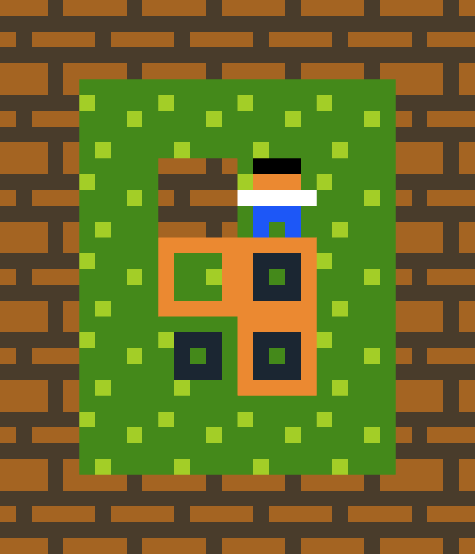
\includegraphics[width=\textwidth]{figures/sokobaniteratelevel.png} \hfill \\
\end{minipage}
$\Longrightarrow$
\begin{minipage}[t]{0.2\textwidth}
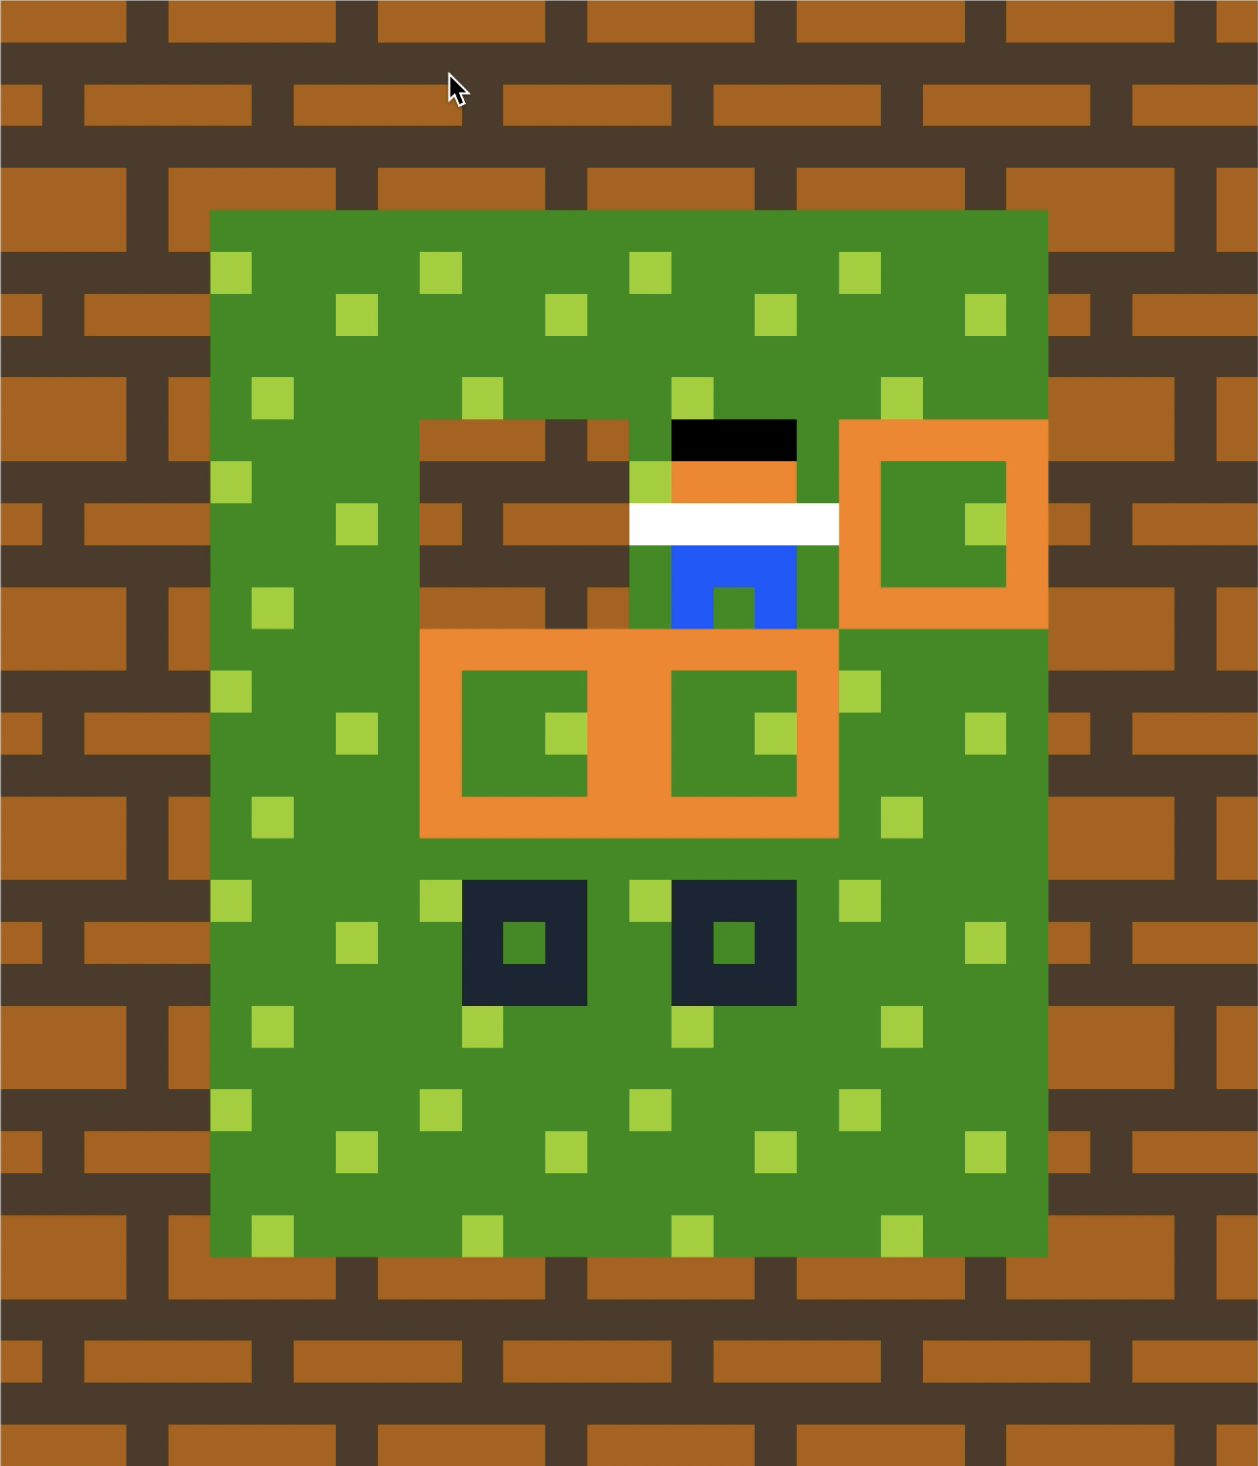
\includegraphics[width=\textwidth]{figures/maxii0.png} \hfill \\
\end{minipage}
$\Longrightarrow$
\begin{minipage}[t]{0.2\textwidth}
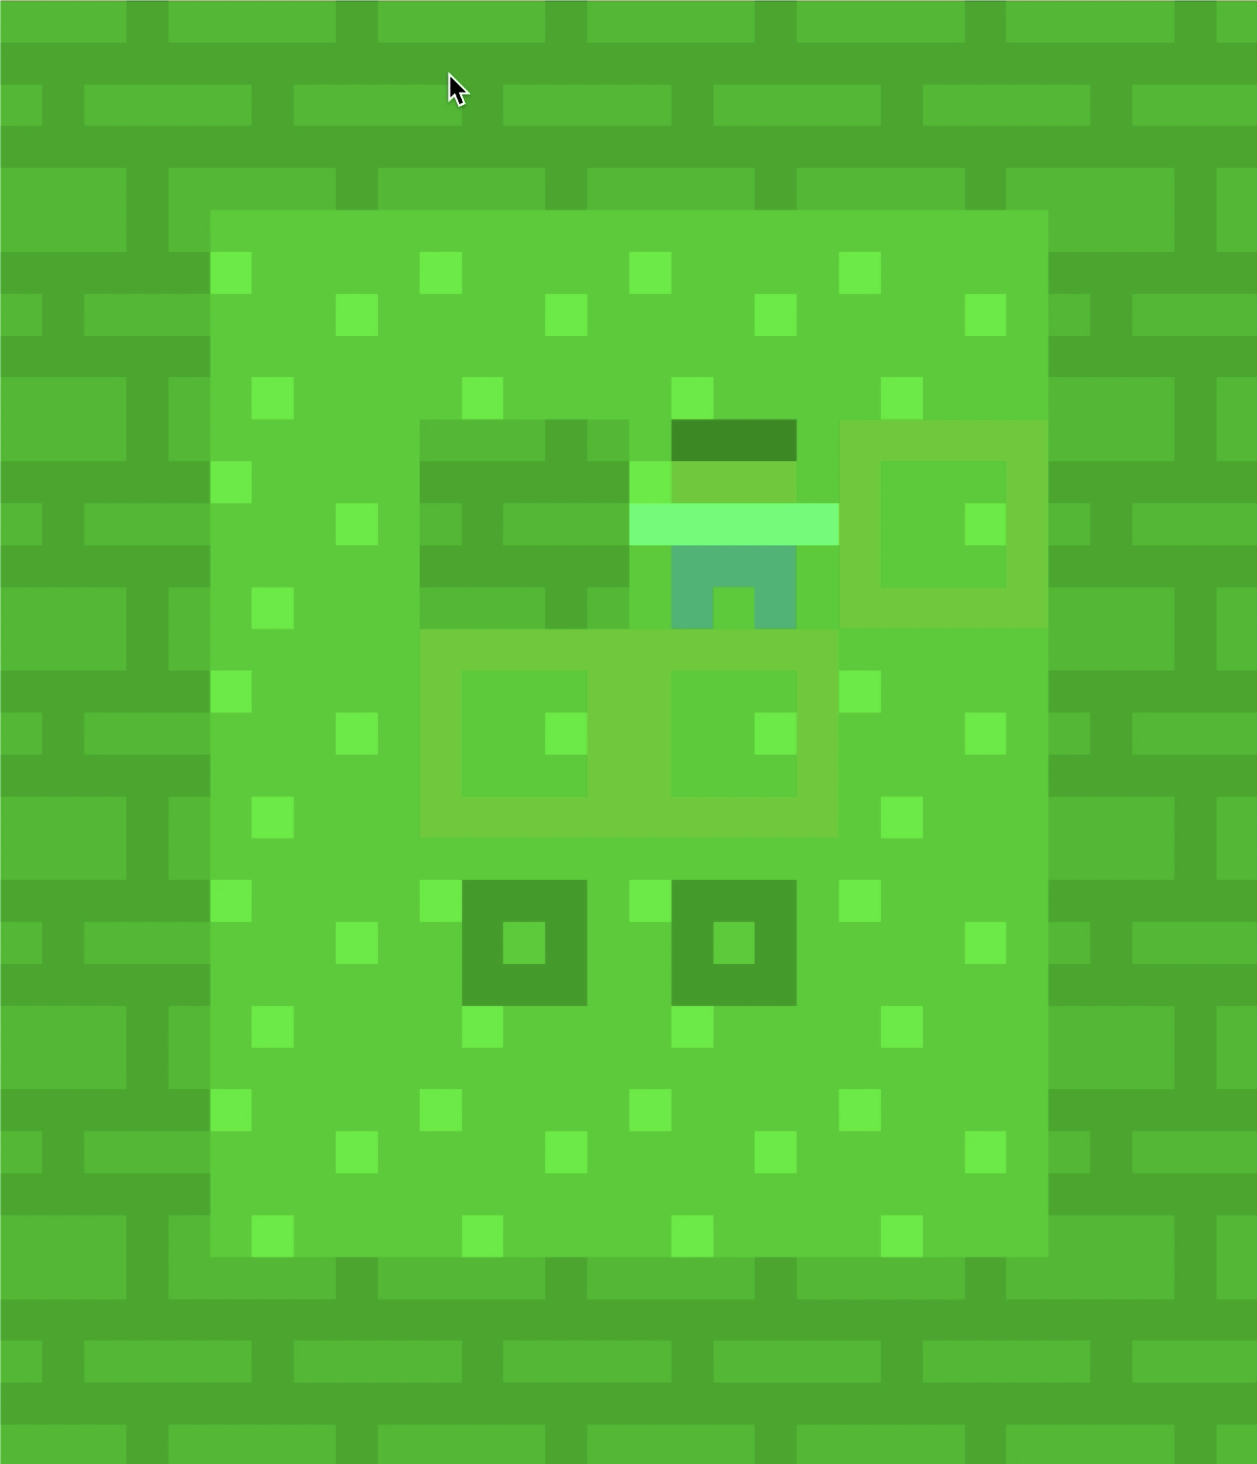
\includegraphics[width=\textwidth]{figures/maxii1_green.png} \hfill \\
\end{minipage}
$\Longrightarrow$
\begin{minipage}[t]{0.2\textwidth}
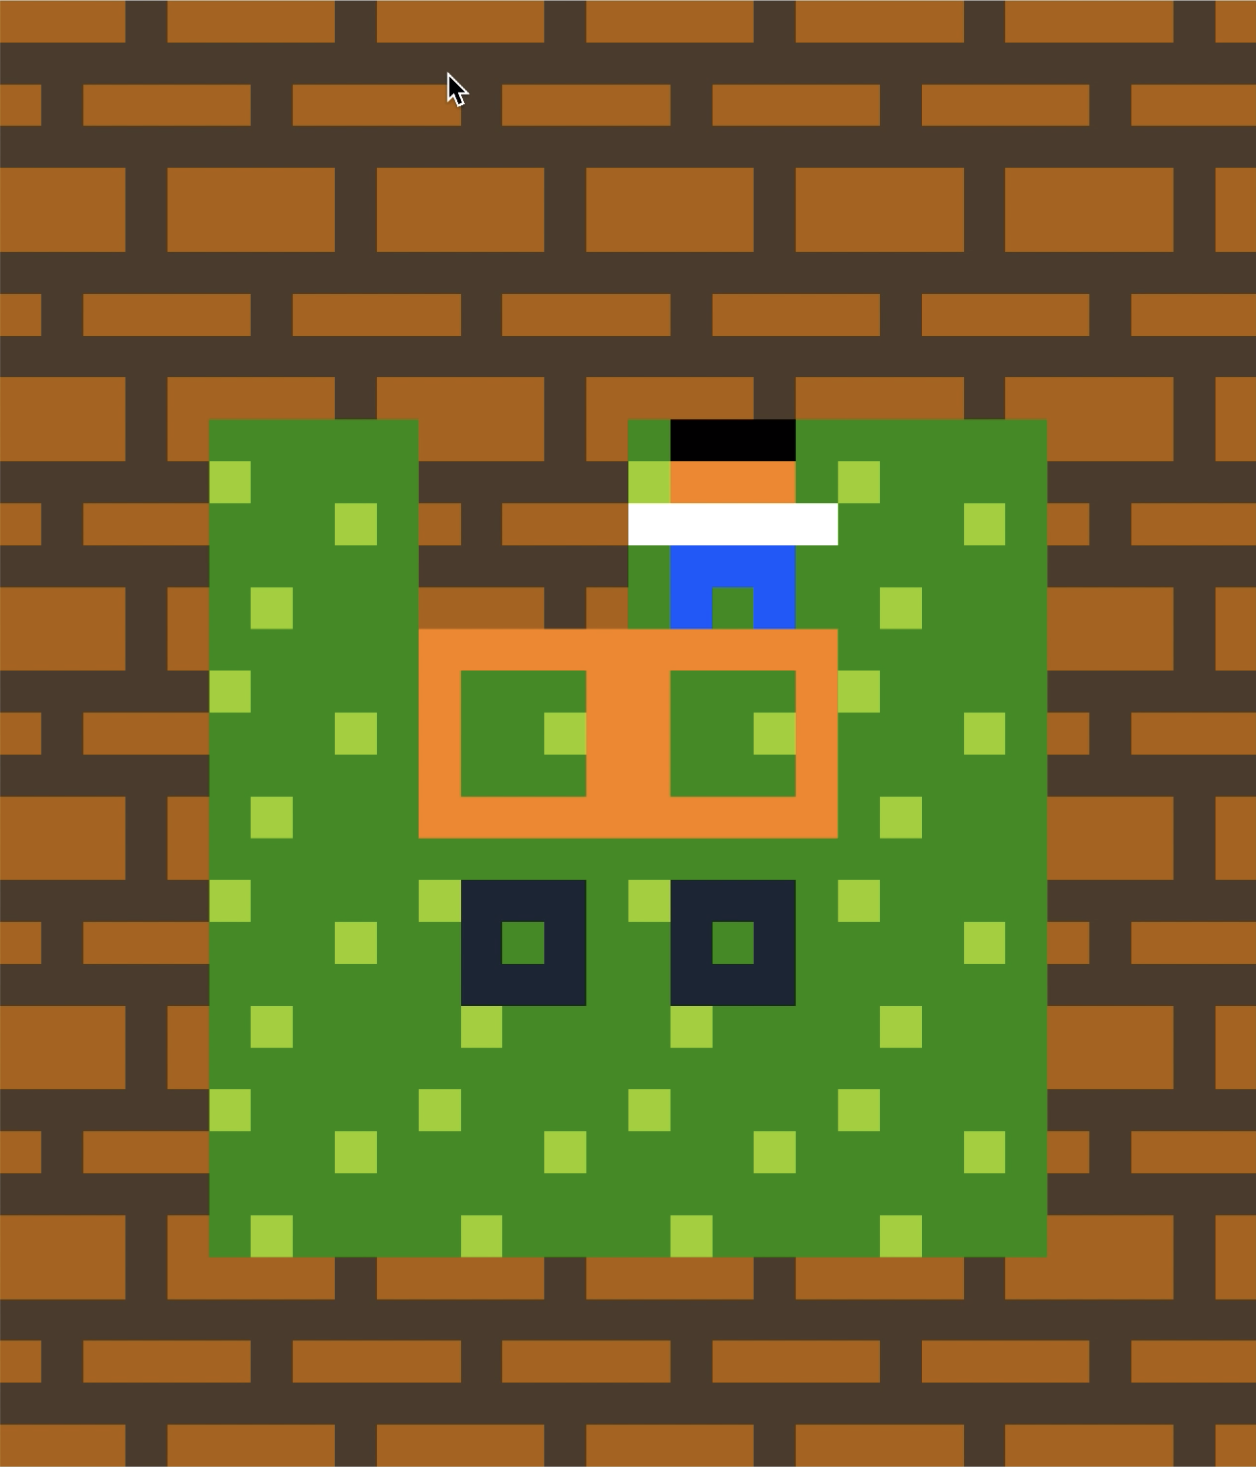
\includegraphics[width=\textwidth]{figures/maxii2.png} \hfill \\
\end{minipage}
$\Longrightarrow$
\begin{minipage}[t]{0.2\textwidth}
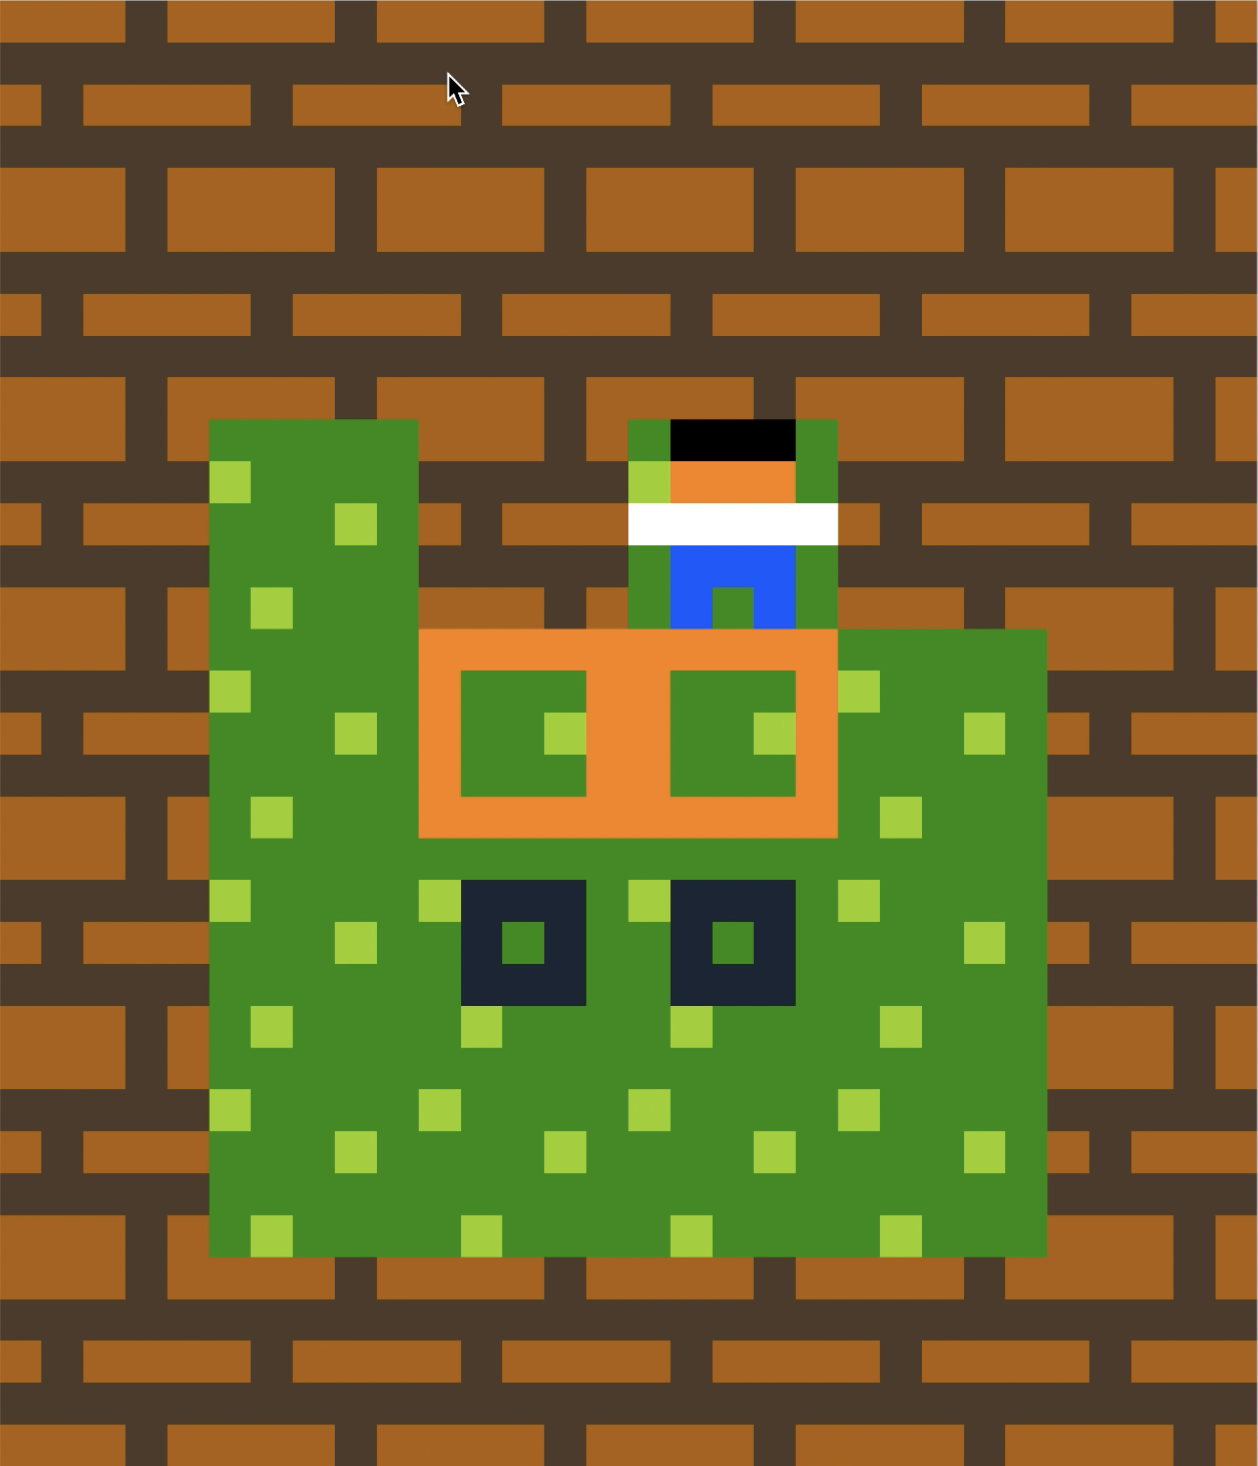
\includegraphics[width=\textwidth]{figures/maxii3.png} \hfill \\
\end{minipage}
$\Longrightarrow$
\begin{minipage}[t]{0.2\textwidth}
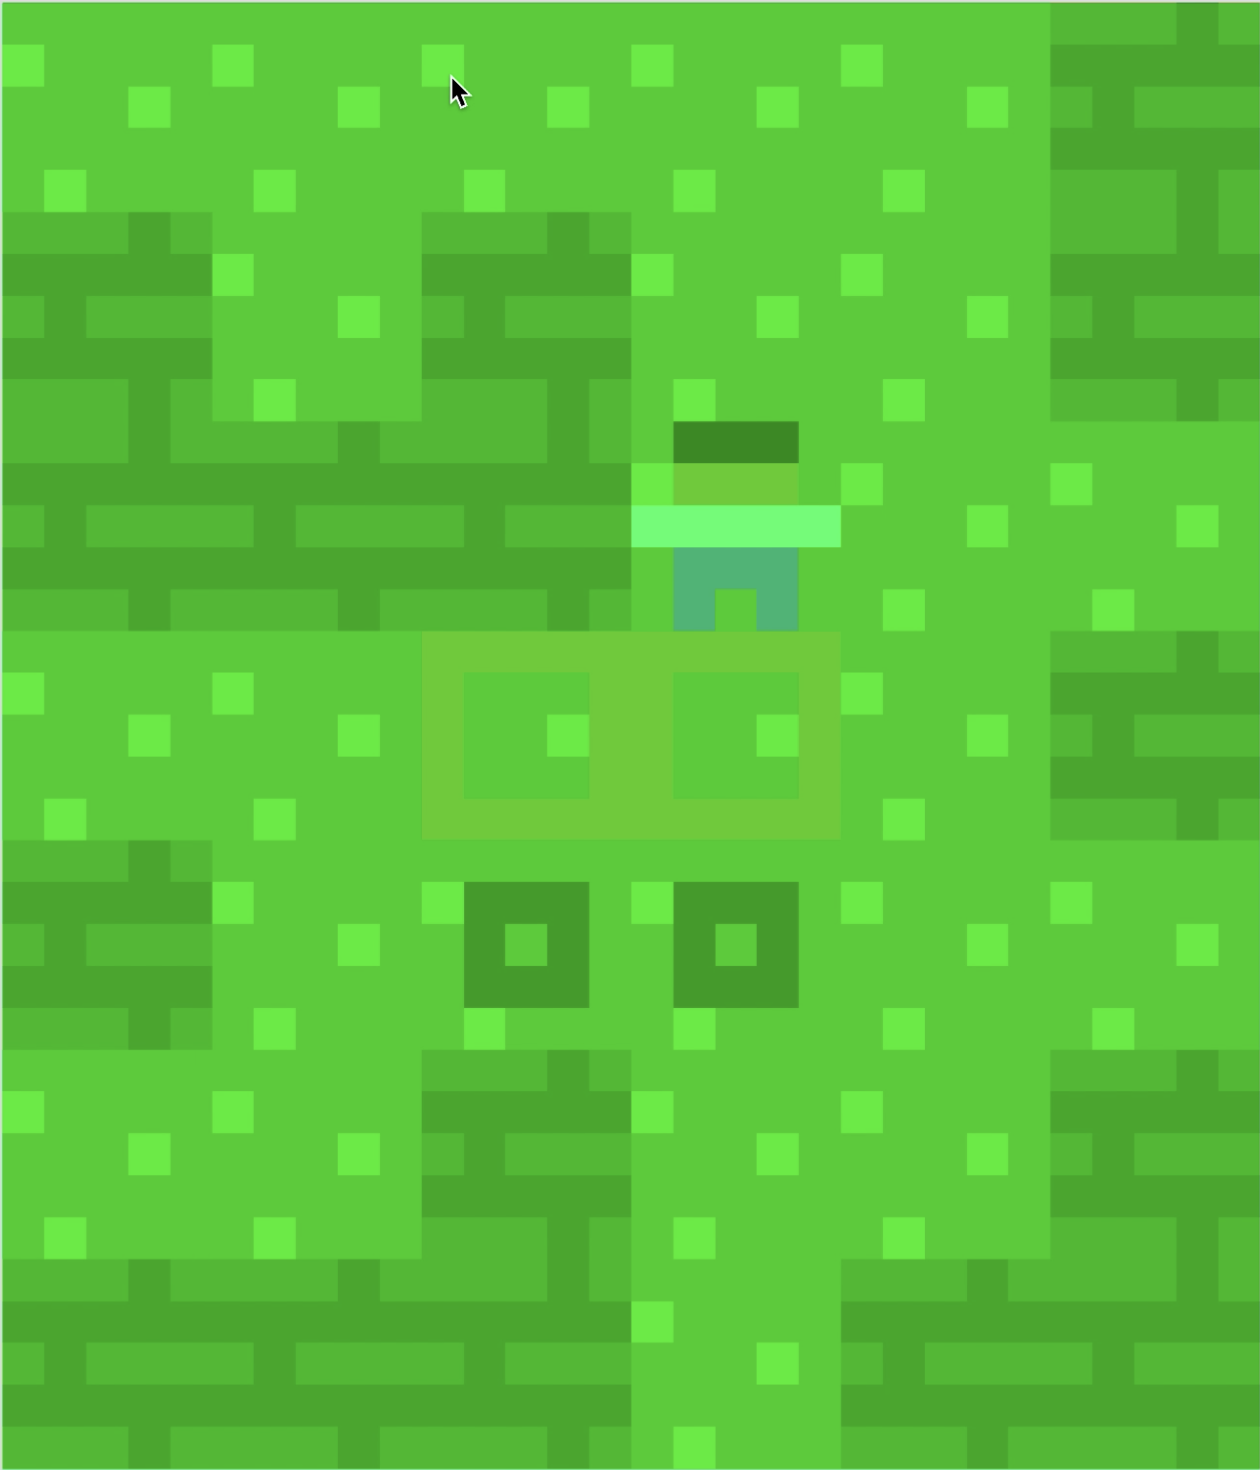
\includegraphics[width=\textwidth]{figures/maxii4_green.png} \hfill \\
\end{minipage}
$\Longrightarrow$
\begin{minipage}[t]{0.2\textwidth}
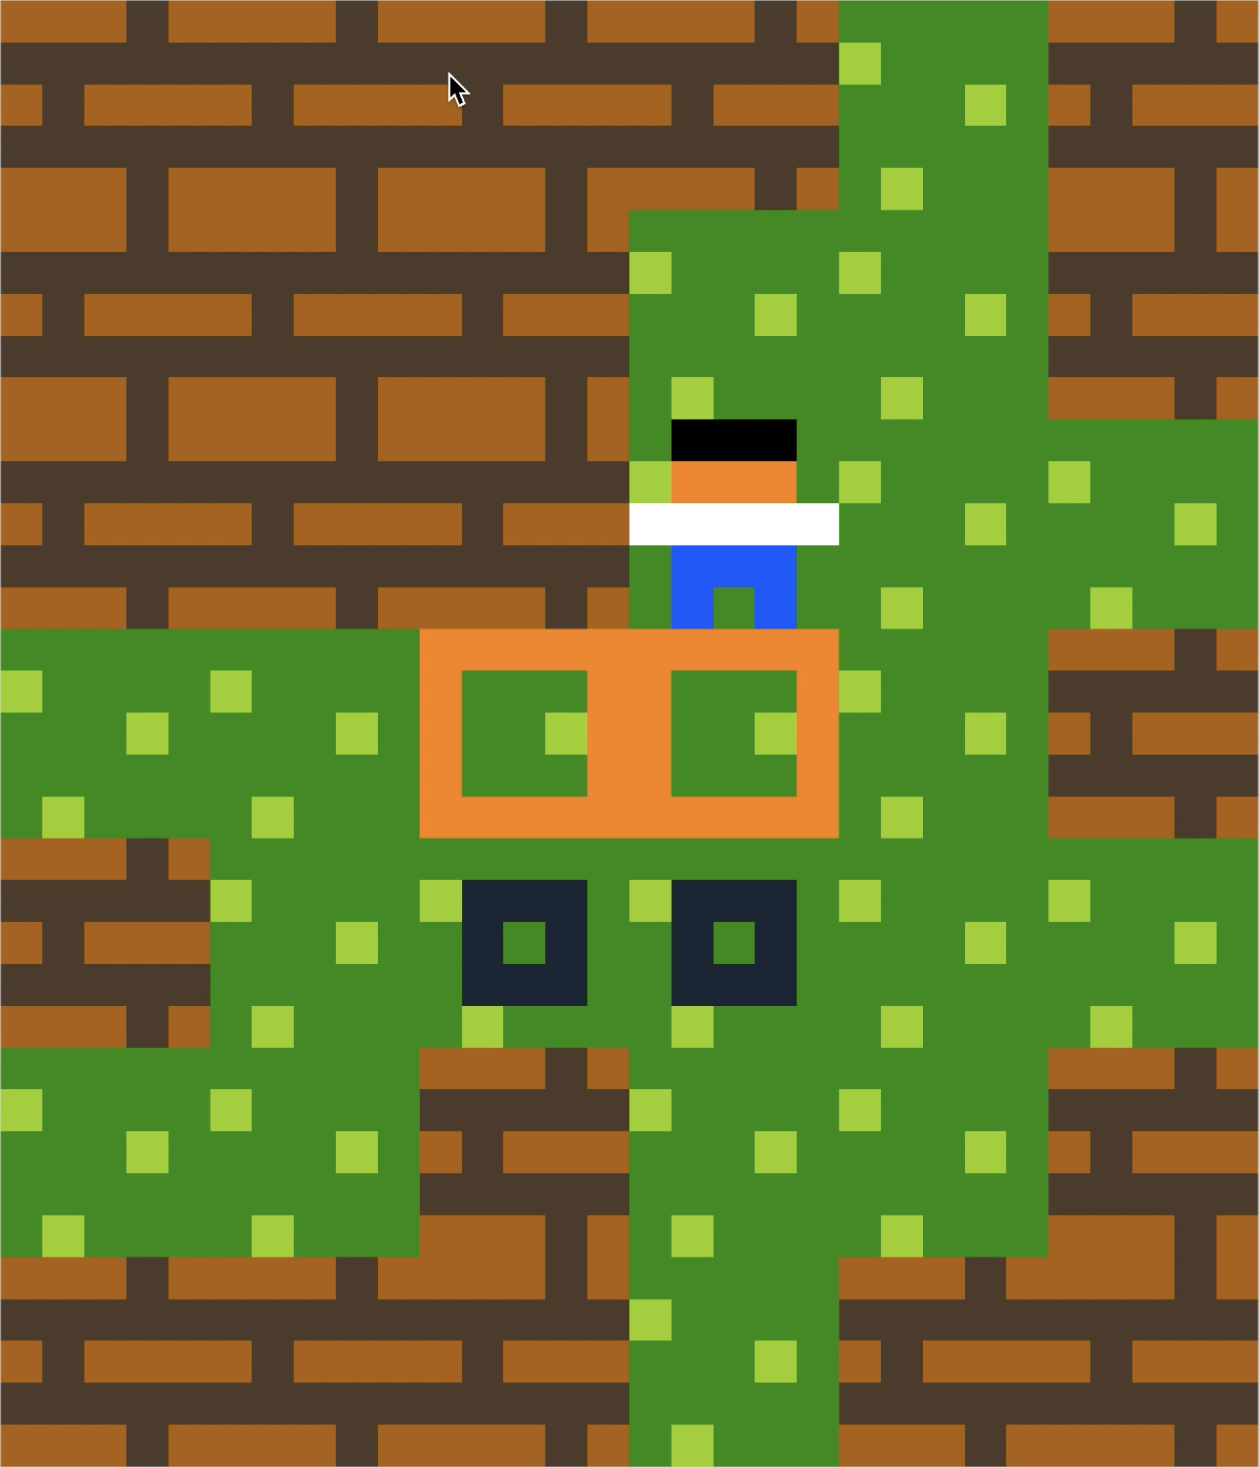
\includegraphics[width=\textwidth]{figures/maxii5.png} \hfill \\
\end{minipage}
$\Longrightarrow$
\begin{minipage}[t]{0.2\textwidth}
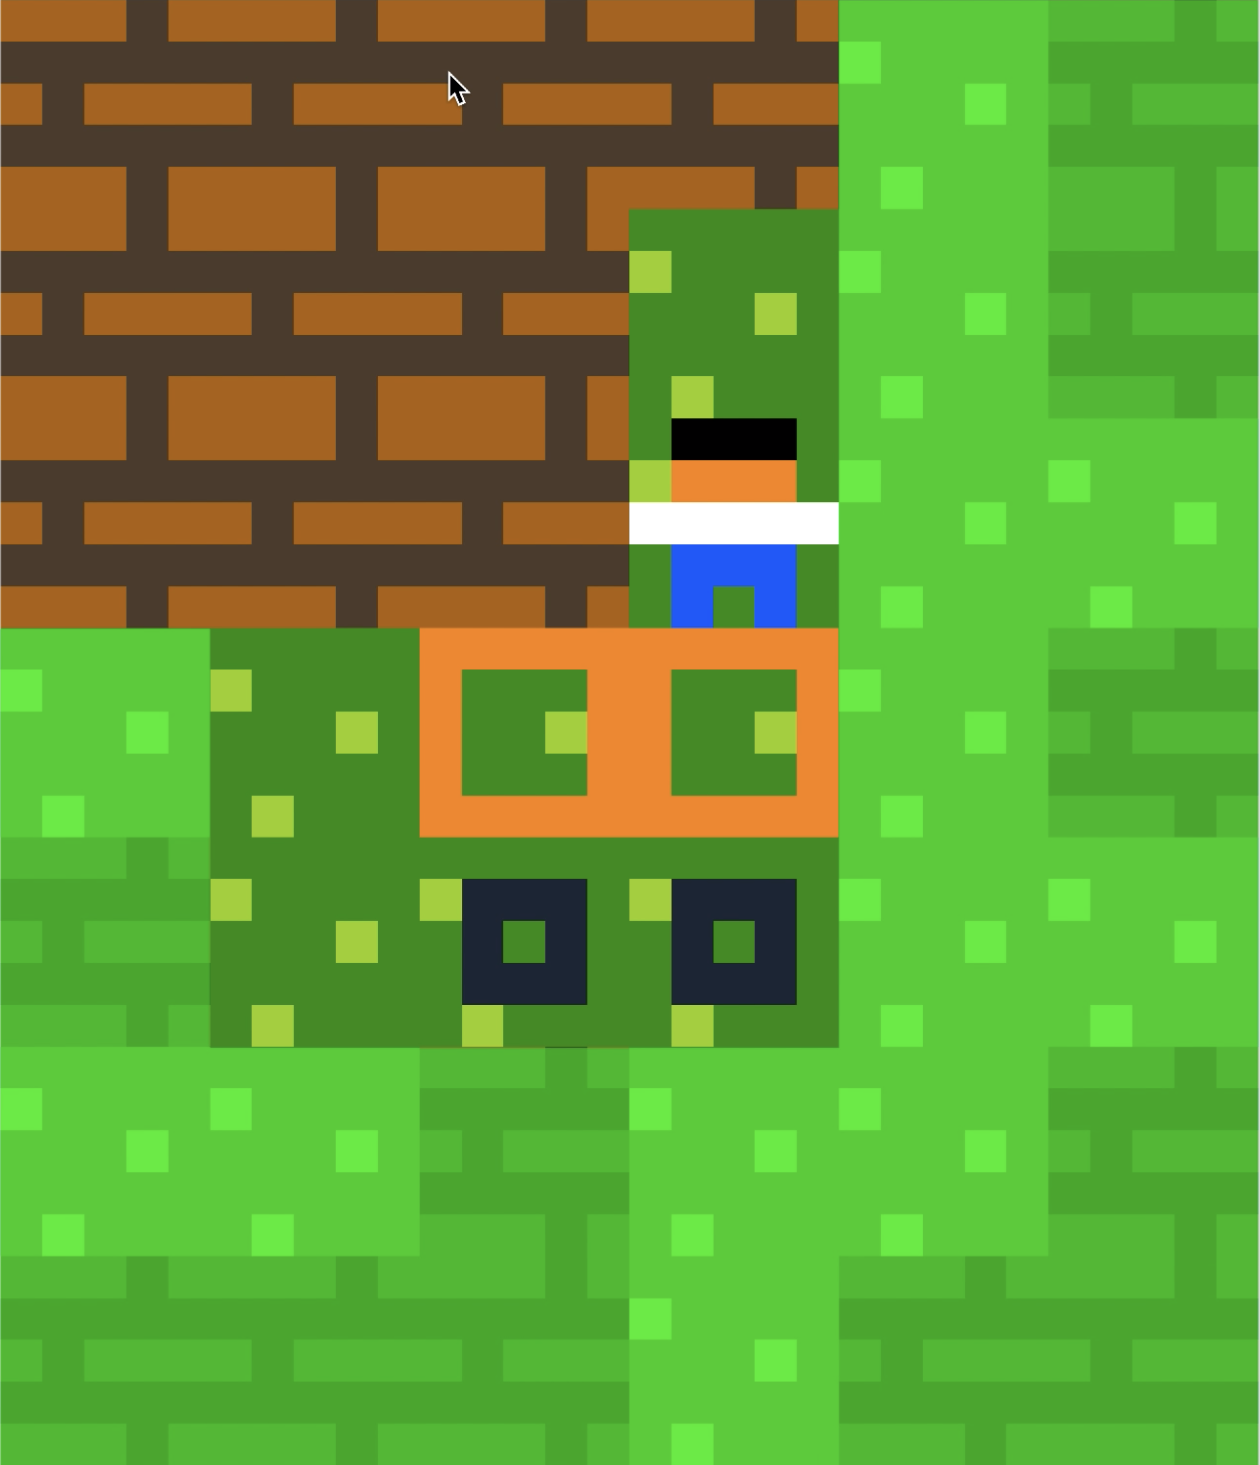
\includegraphics[width=\textwidth]{figures/maxii6.png} \hfill \\
\end{minipage}
$\Longrightarrow$
\begin{minipage}[t]{0.2\textwidth}
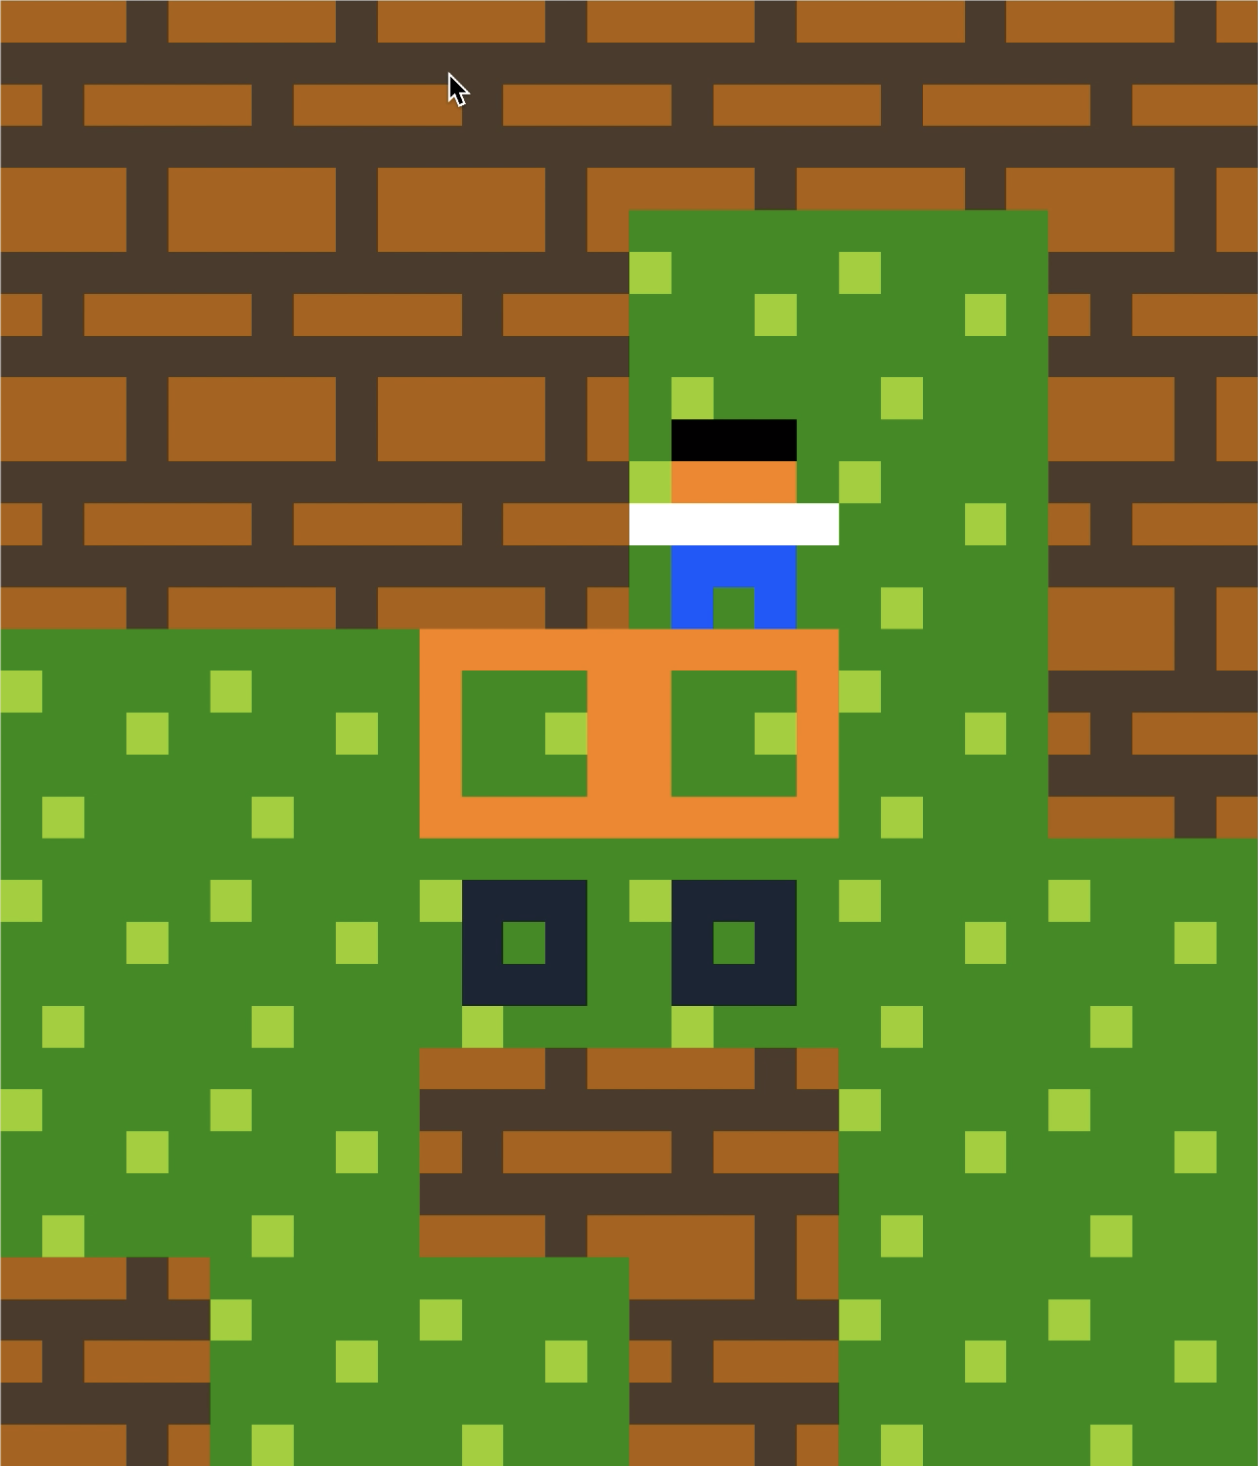
\includegraphics[width=\textwidth]{figures/maxii7.png} \hfill \\
\end{minipage}
$\Longrightarrow$
\begin{minipage}[t]{0.2\textwidth}
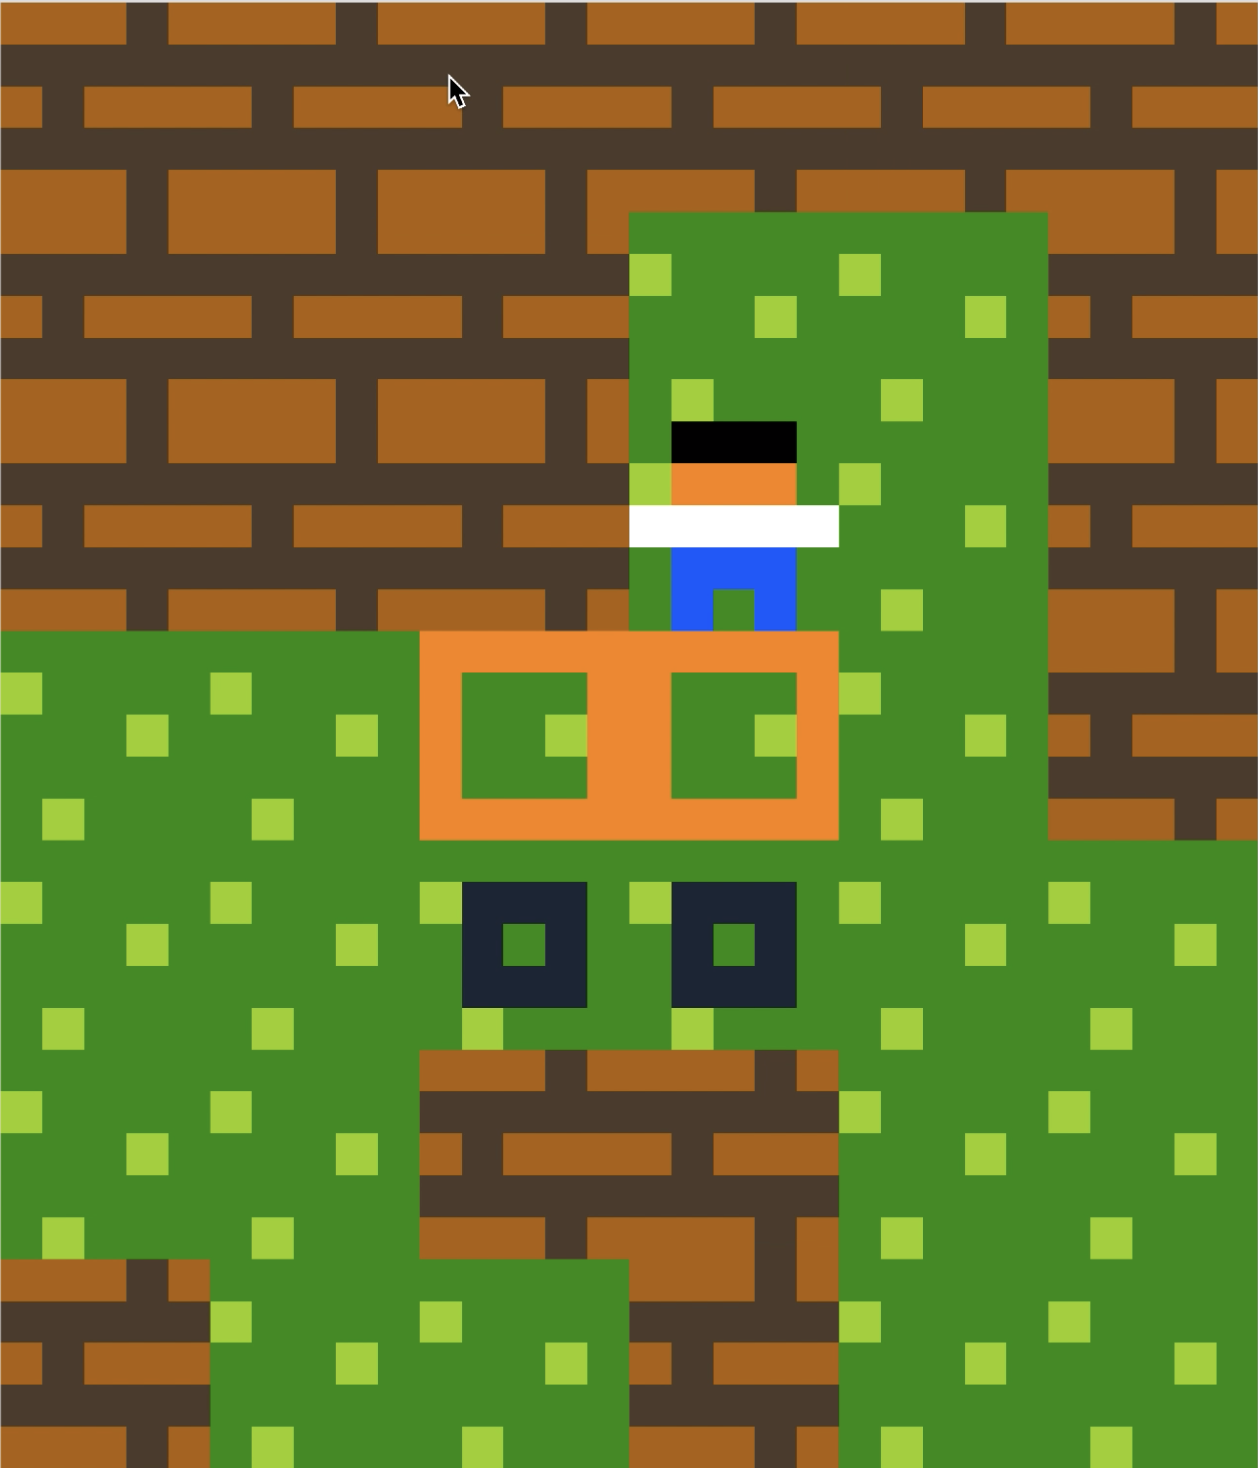
\includegraphics[width=\textwidth]{figures/maxii8.png} \hfill \\
\end{minipage}
\caption{Participant 6: Iterative design processed \label{fig:part6iterative}}
\end{figure}



\begin{figure}[!htbp]
\begin{minipage}{0.5\textwidth}
\centering
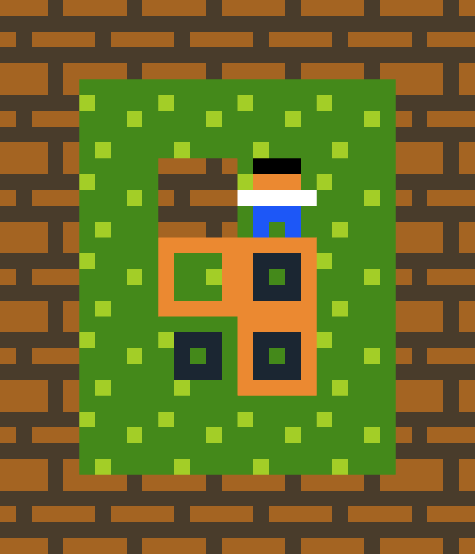
\includegraphics[width=0.55\textwidth]{figures/sokobaniteratelevel.png}

\end{minipage}  $\Longrightarrow$ \hfill
\begin{minipage}{0.4\textwidth}
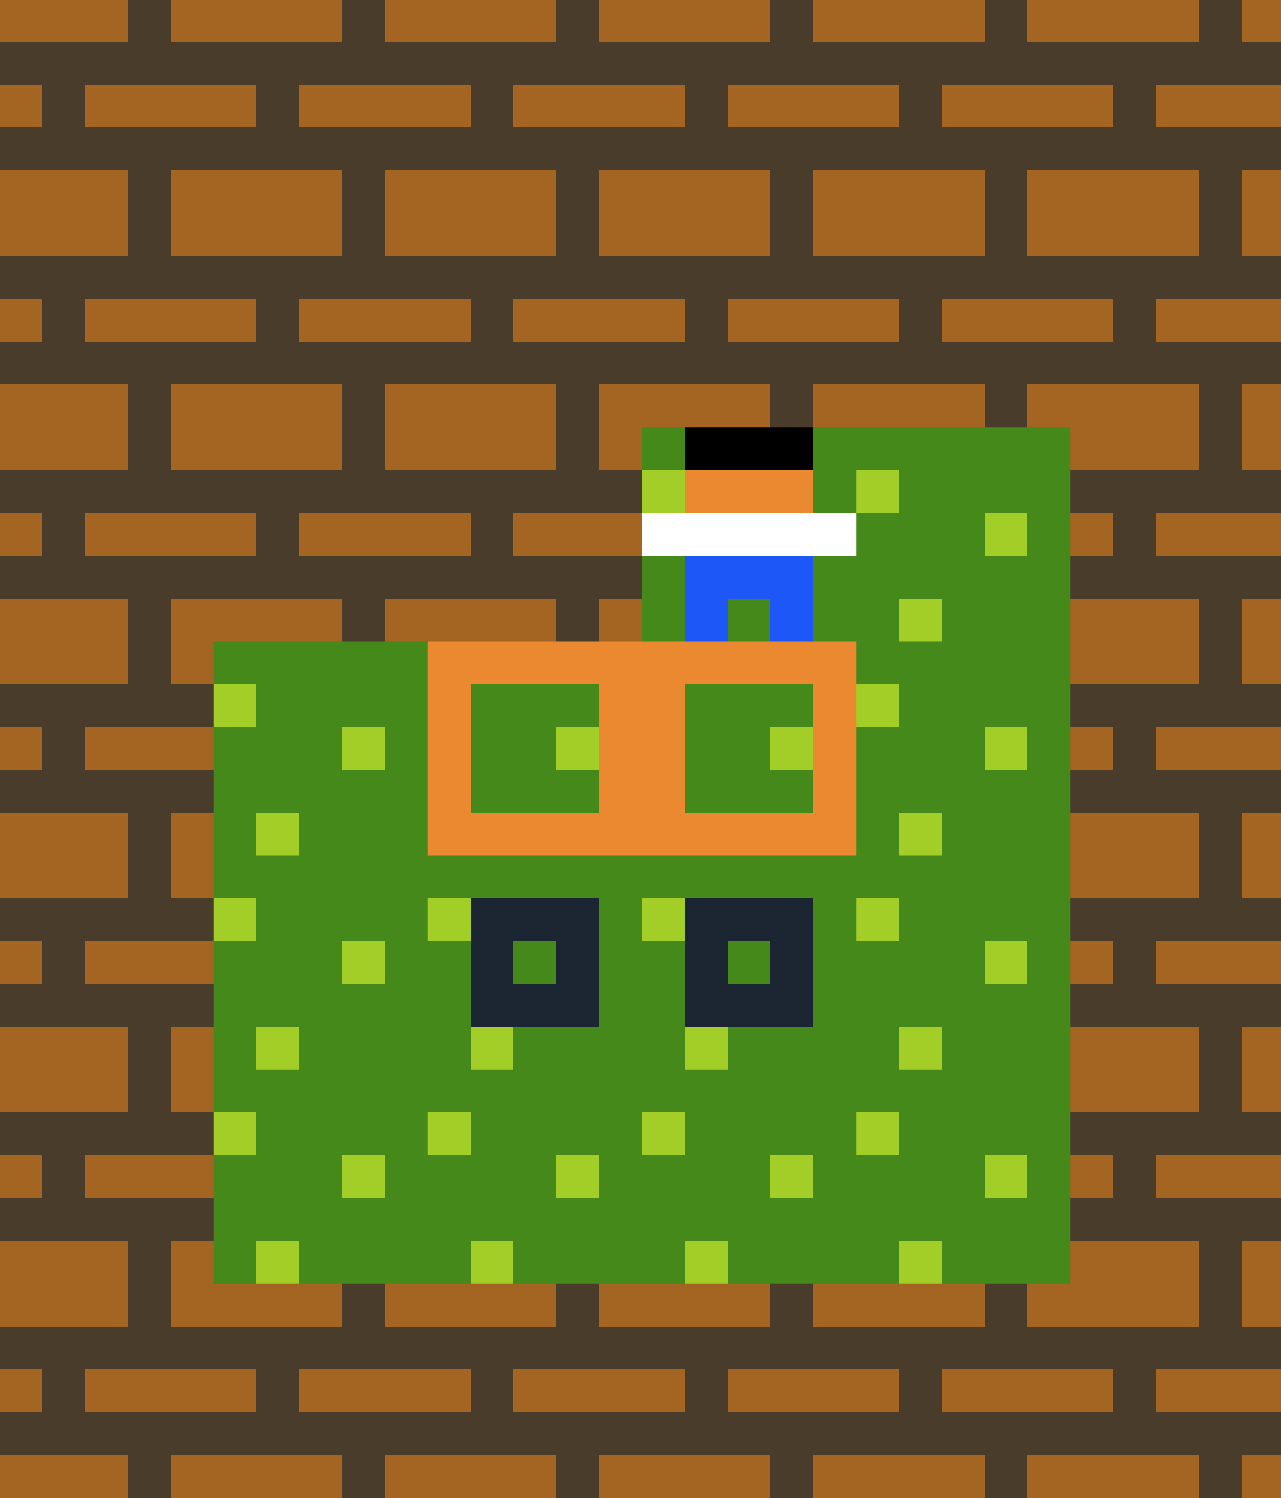
\includegraphics[width=0.55\textwidth]{figures/firstmax_without.png} \hfill \\
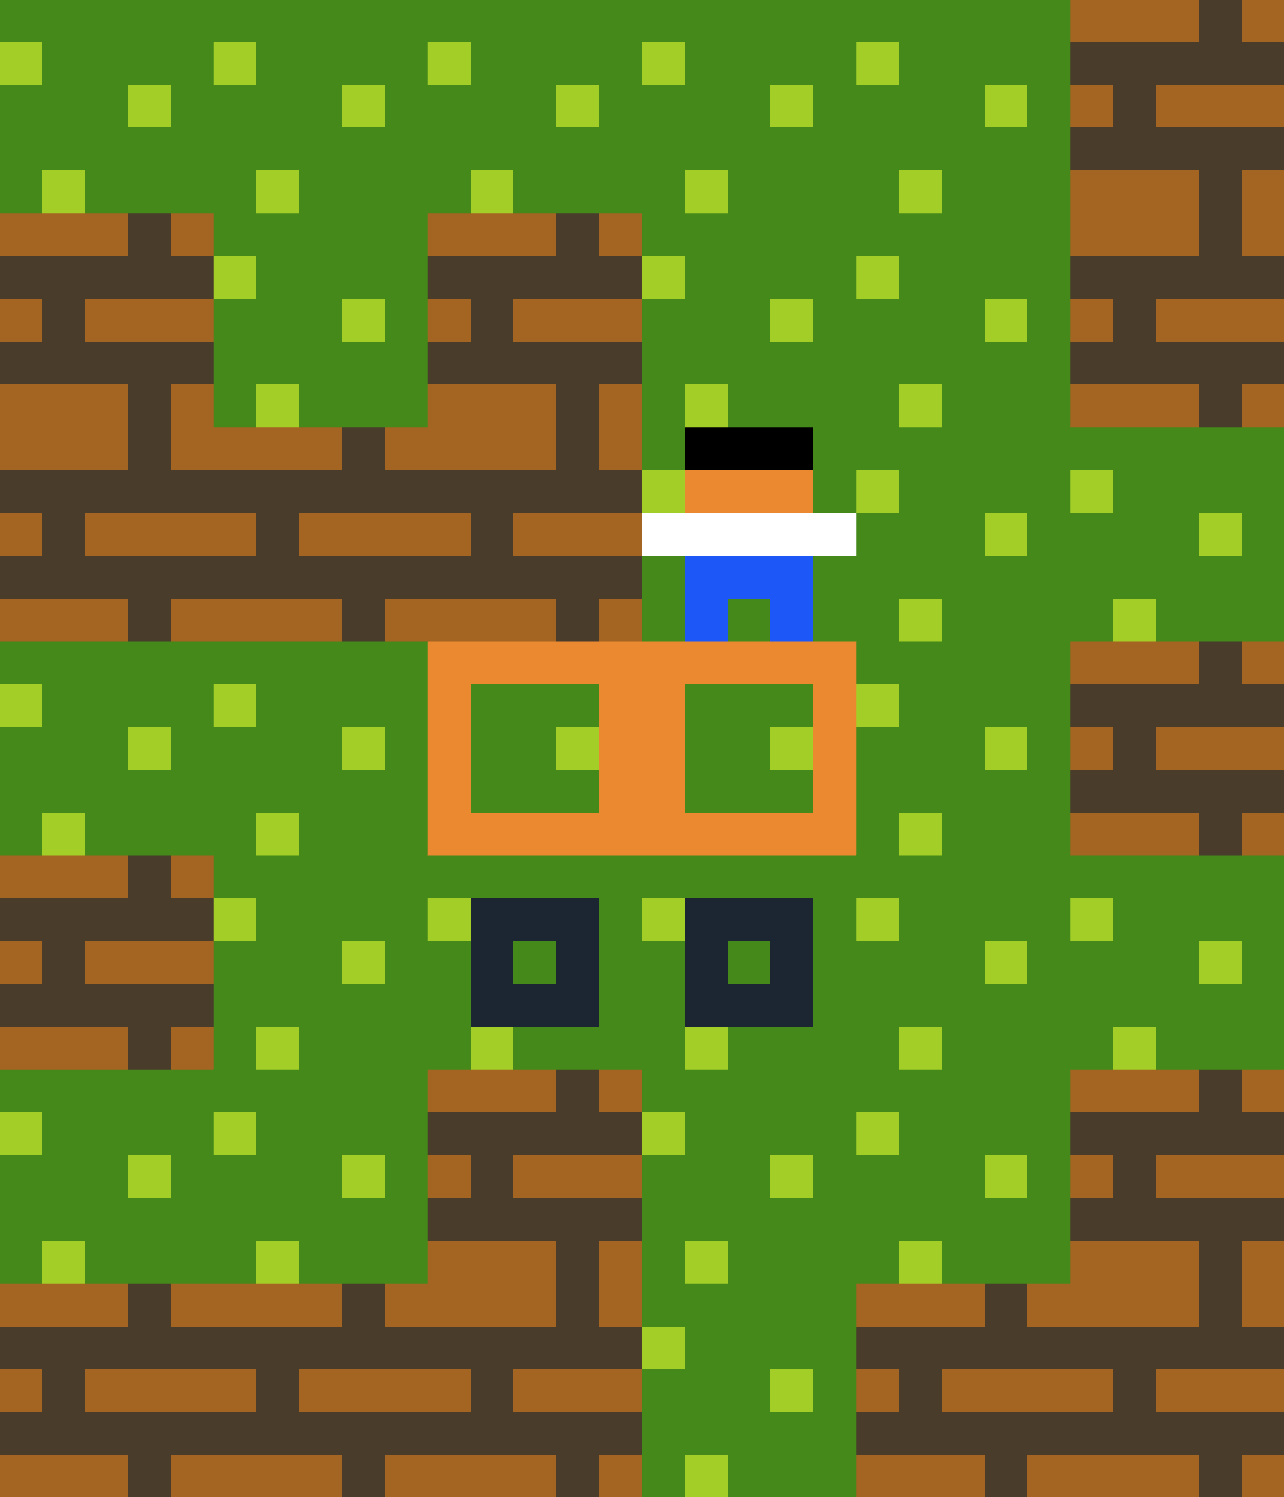
\includegraphics[width=0.55\textwidth]{figures/secondmax_without.png} \hfill \\
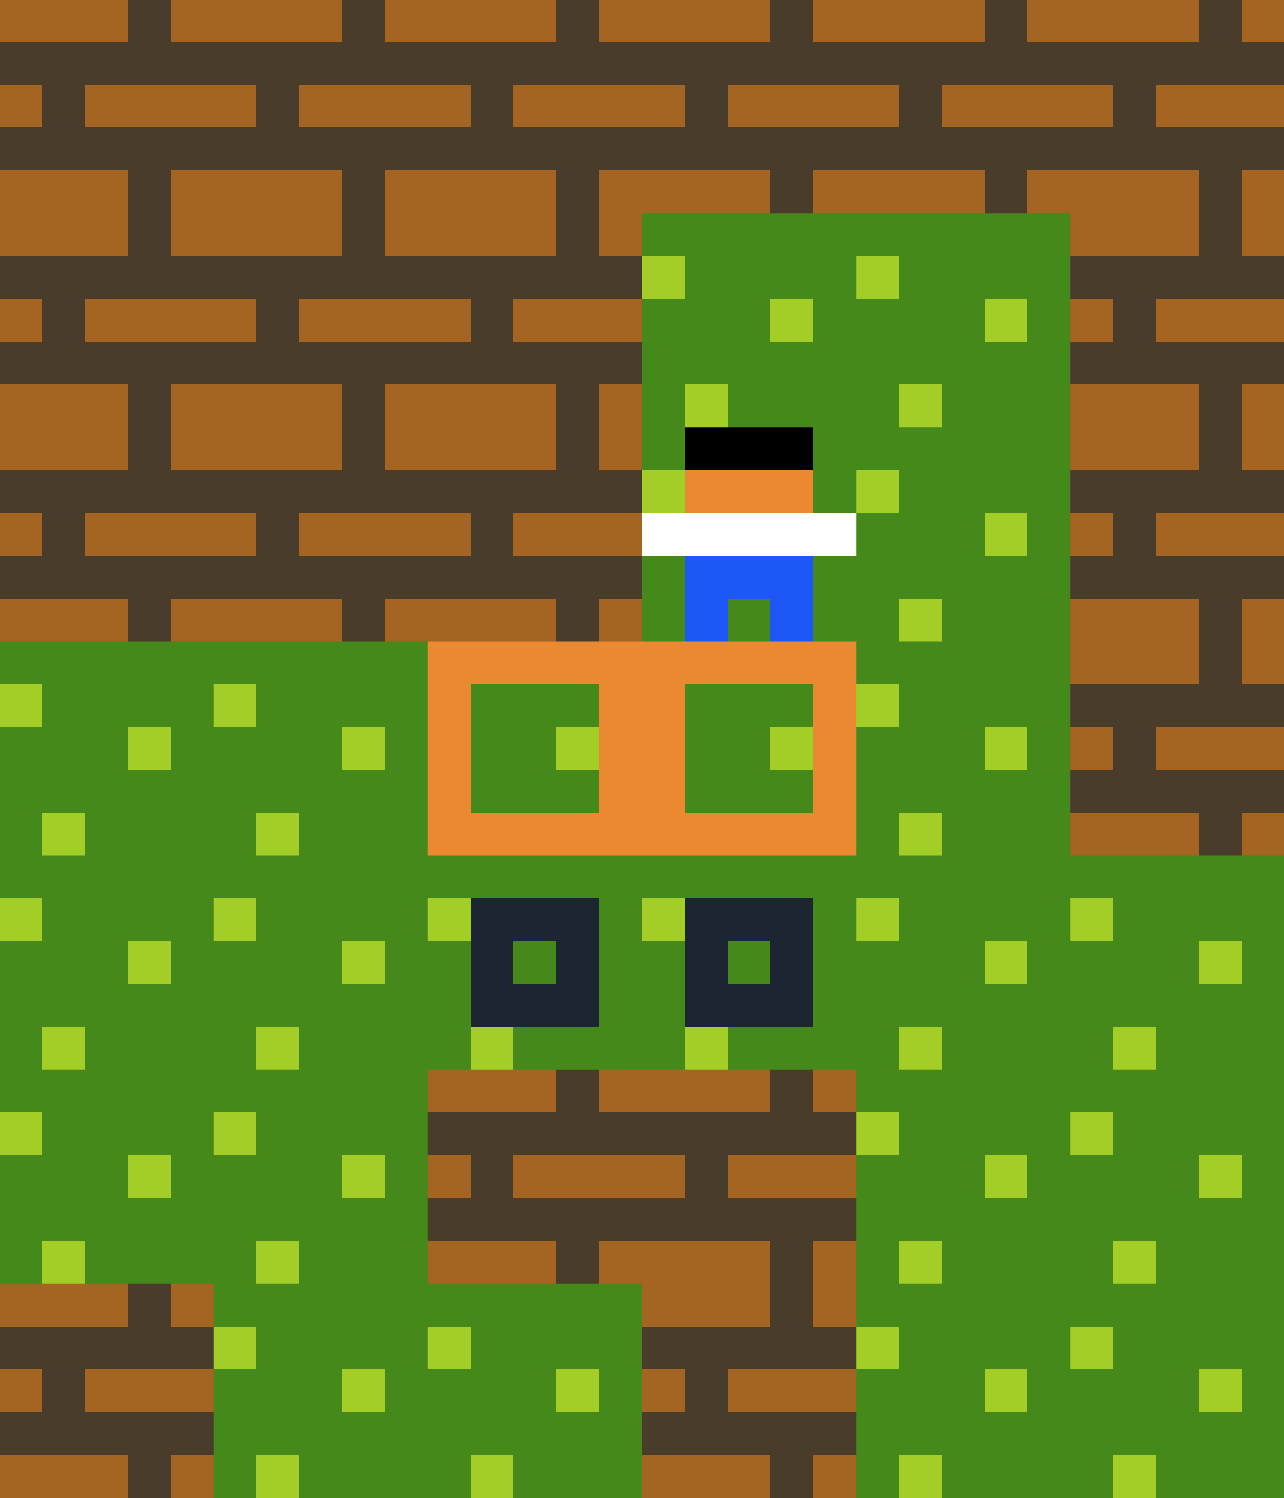
\includegraphics[width=0.55\textwidth]{figures/thirdmax_without.png} \hfill \\
\end{minipage}
\caption{Participant 6: Final iterative designs}
\end{figure}


\begin{figure}[!htbp]
\centering
\begin{minipage}[t]{0.2\textwidth}
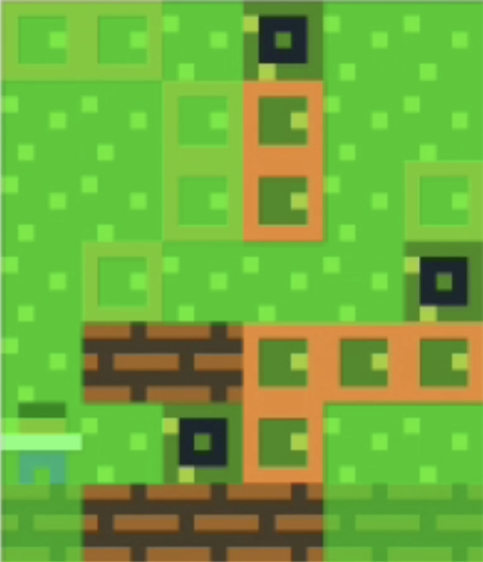
\includegraphics[width=\textwidth]{figures/p8greena.png} \hfill \\
\end{minipage}
$\Longrightarrow$
\begin{minipage}[t]{0.2\textwidth}
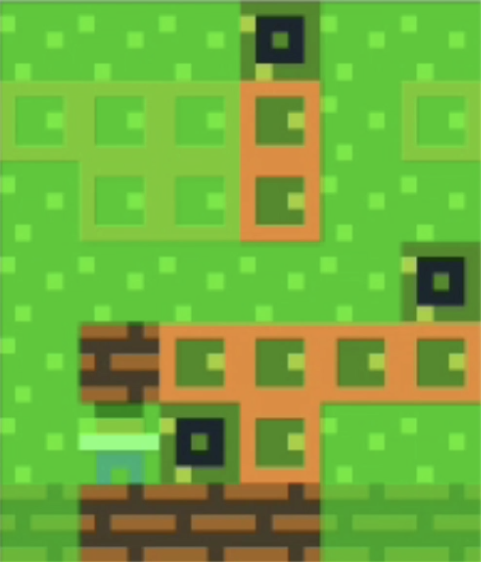
\includegraphics[width=\textwidth]{figures/p8greenb.png} \hfill \\
\end{minipage}
$\Longrightarrow$
\begin{minipage}[t]{0.2\textwidth}
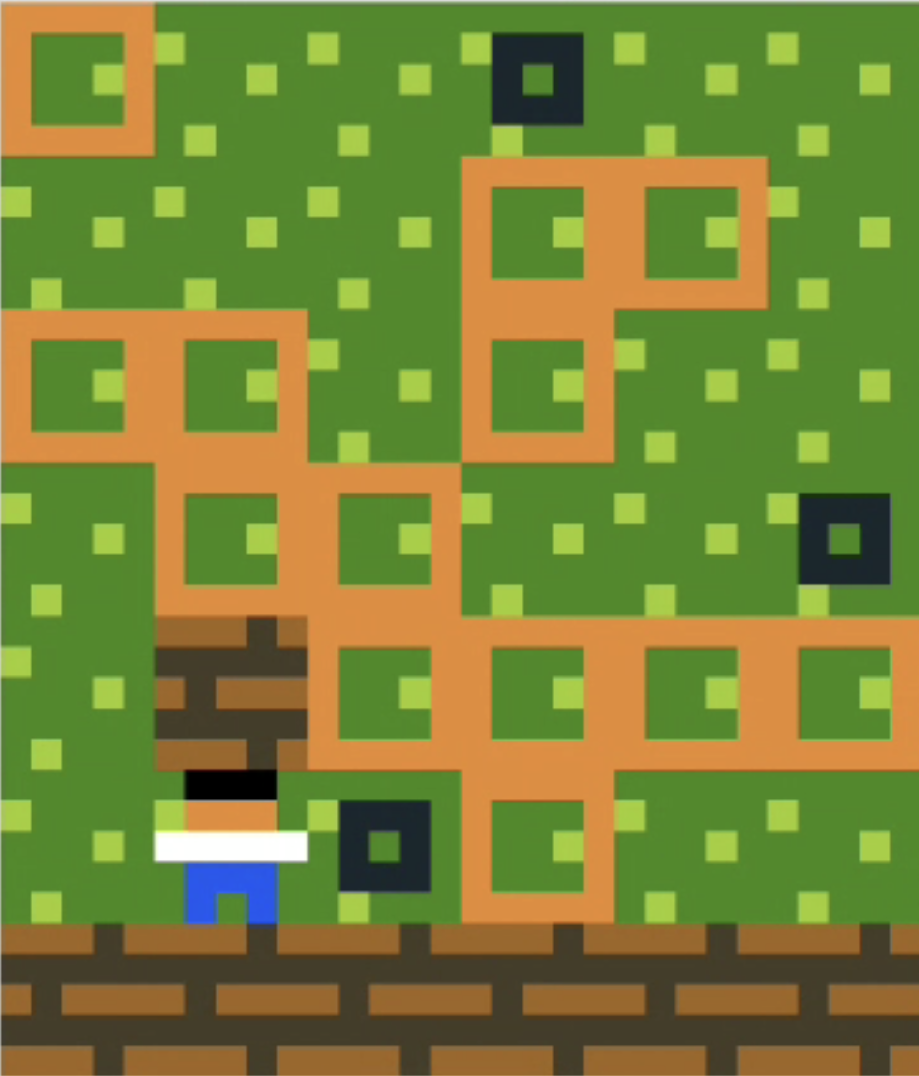
\includegraphics[width=\textwidth]{figures/p8greenc.png} \hfill \\
\end{minipage}

\caption{Participant 7: Iterative design process}
\end{figure}


\subsection{Design patterns}

In this section, we list design patterns for the iterative design approach which we obtained from the think-aloud study and see in which way participants profit from mixed-initiative methods.


\begin{description}
\item[Identifying aesthetics/mechanics] After using the tool for a while, a lot of our participants have found \textit{aesthetically} pleasing sections or \textit{mechanically} interesting sections upon which they liked to expand on. For example, participant 6 liked the two targets and crates in the design mentioned above.

%Especially participant 1, 2 \& 4 have used the tool mostly for this purpose considerable time with the other aspect of the mixed-initiative tool: Finding it for inspiration.

% They then continue to expand on it with creative constraints, window dress the solution or try to transform a given design using the generator.

MixedAim helped the designer identify some interesting designs by passively suggesting levels during the design phase (5 participants claimed they got inspired by a level without clicking on it) or by the designer explicitly looking for them with the transformer. Especially participants 1, 2 \& 4 focused on using the transformer to come up with original designs upon which they then were able to improve, see also the section 5.1.3. 

\item[Creative constraints] These are situations where designers constrain themselves only to the use of a previously identified aesthetic or mechanic. Every participant worked with creative constraints in one way or the other.

Mixed-initiative tools helped the designer to satisfy \textit{aesthetic constraints} by allowing them to \textit{freeze} certain sections that the transformer would not be able to change. For example, participant 6 decided he would keep the two crates and the two walls and constrained the transformer to only change the level around the crate target pairs. Further suggestions for \textit{aesthetic constraints} followed from the structured interview included adding tools for \textit{symmetry} and being able to \textit{combine} two levels in interesting ways.

For \textit{mechanical constraints}, the transformer rules have to be employed to create interesting mechanics. These are for example the preset buttons like only moving the crates or removing/adding some walls and keeping the rest intact. Suggestions included not only \textit{specifying} ways of transforming but also specifying means of constraining allowed transformations. 

\item[Unsolvable into solvable] This was not something we encountered in the literature, but it was something that happened very frequently with our mixed-initiative system. As soon as designers were passively shown that the level was unsolvable, they did not spend the effort to make it solvable manually but simply told the tool to make the current design work somehow. A lot of these designers then reported being pleased by the methods the transformer came up with to make the level solvable again.

This was also mentioned directly by participant 3 during the think-aloud study: \textit{\say{A perfect way to use this [tool] is if you find something that looks interesting, but you can't quite get it to be solvable or something like that.}}

\begin{figure}[!htbp]
\begin{minipage}{0.5\textwidth}
\centering
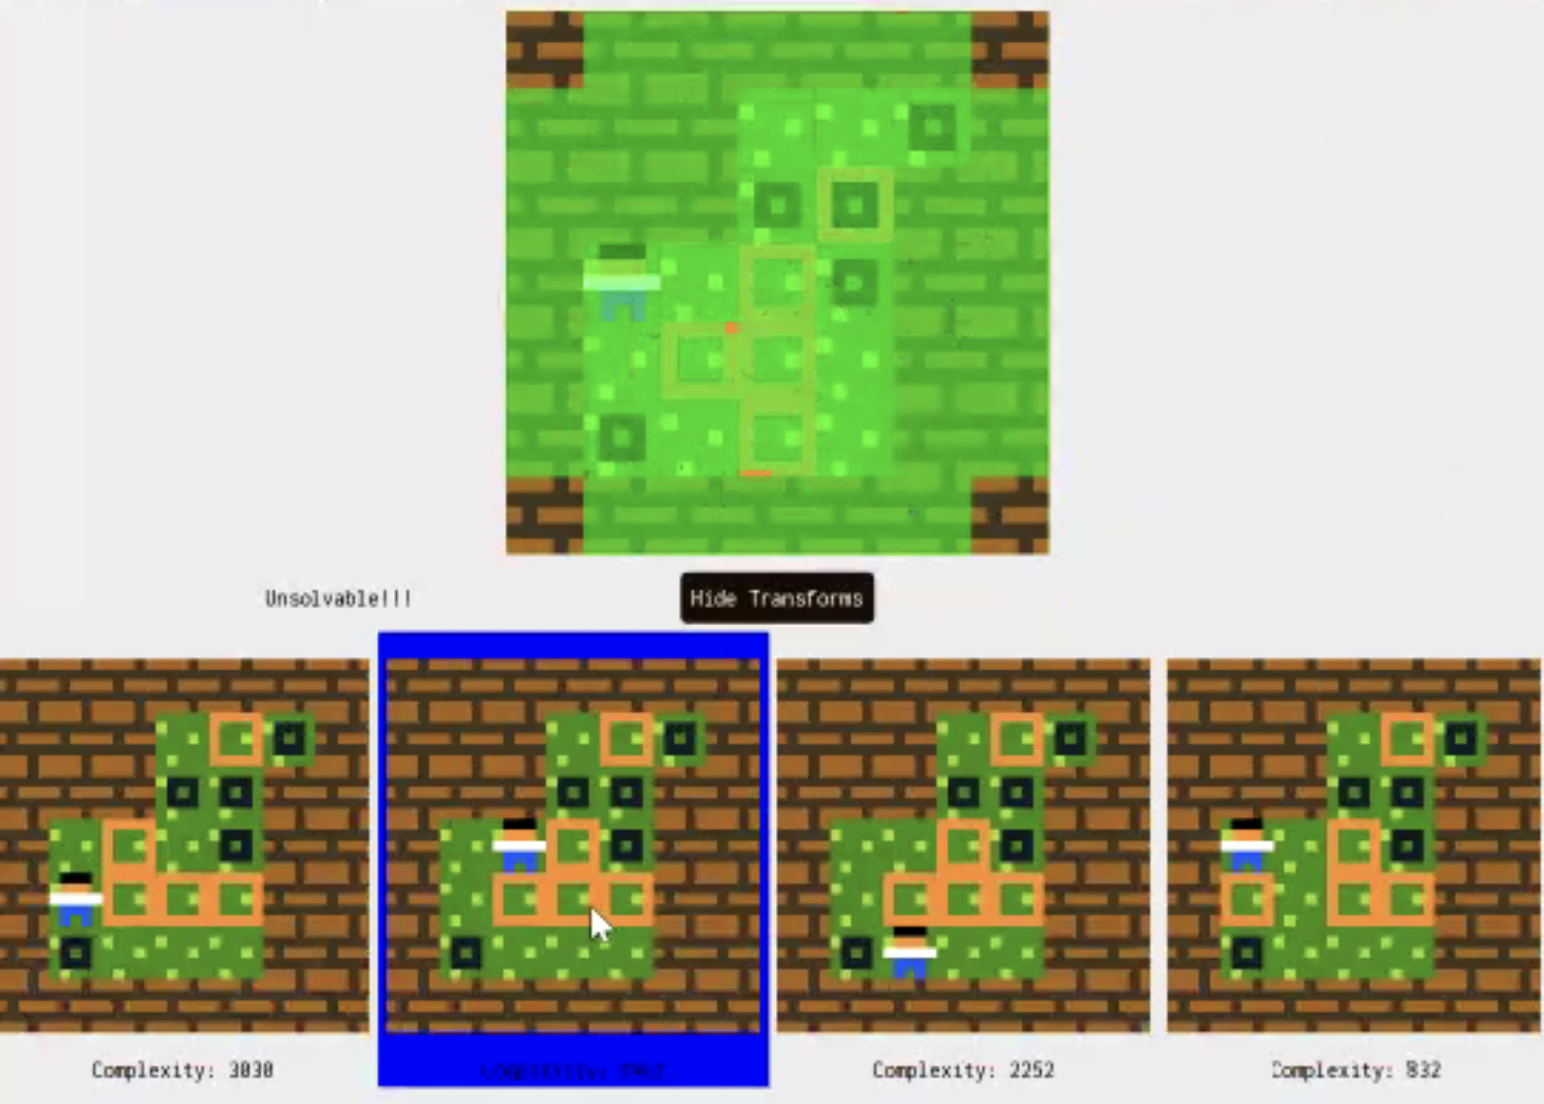
\includegraphics[width=\textwidth]{figures/unsolvablepart4.png}
\end{minipage}  \hfill
\begin{minipage}{0.5\textwidth}
\centering
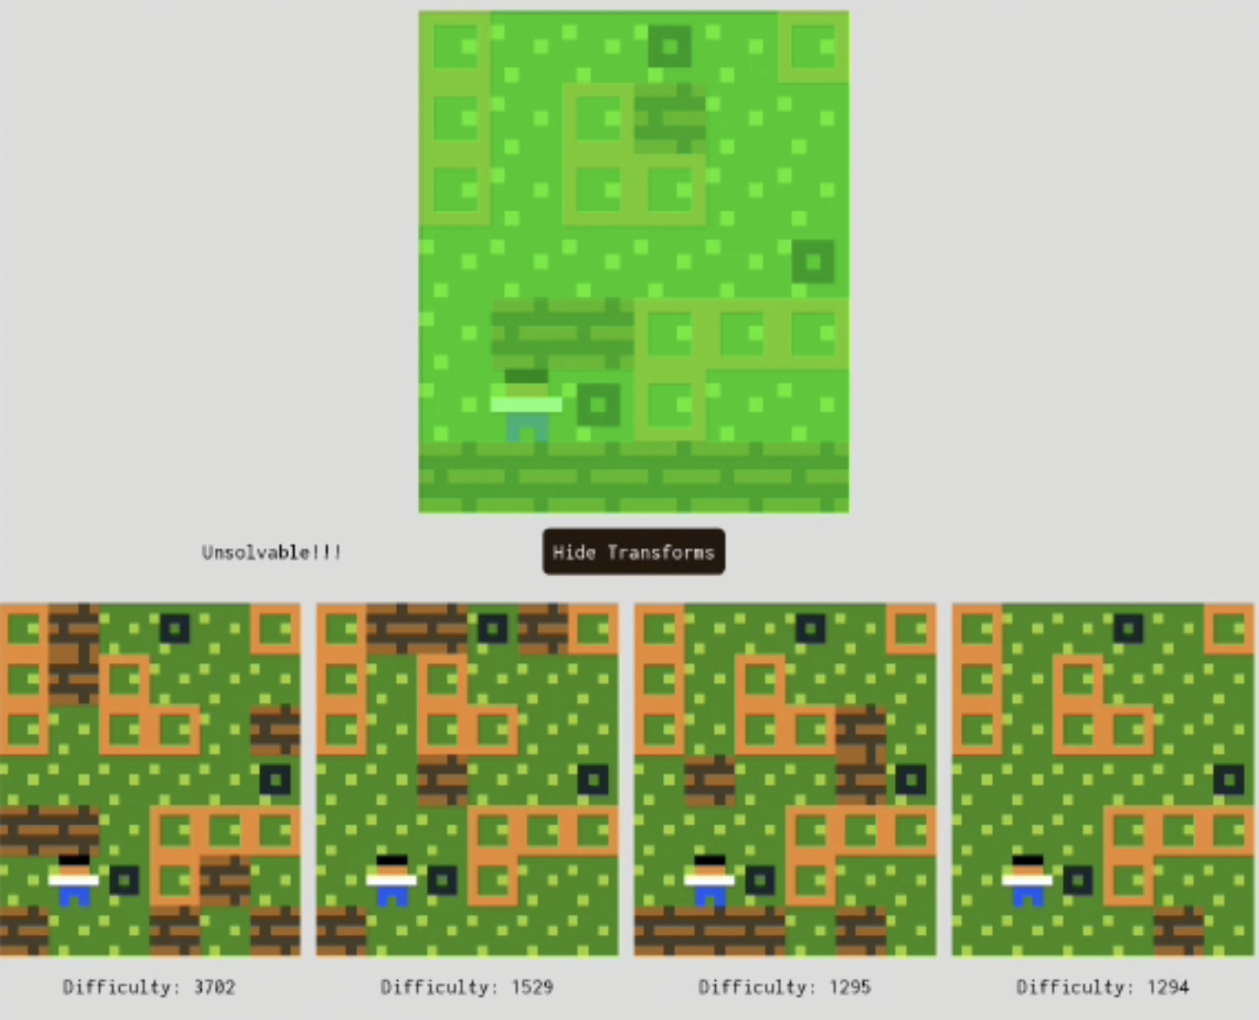
\includegraphics[width=\textwidth]{figures/unsolvablepart72.png}
\end{minipage}
\caption{Participant 4 \& 7: Unsolvable to solvable}
\end{figure}

\item[Window dressing] This happens when an interesting level is found (through the transformer or the designer) that contains a lot of unnecessary states. The designer then tries to eliminate all these unnecessary states (without making the problem trivial) to find the `canonical form', the `kernel' of the problem. It was mentioned by participant 1, 6 \& 7.
%definitely mentioned by participant 1, participant 6, thatscar and participant 7.

Our mixed-initiative tools only help to address this problem in so far that they help the designer to edit the level quickly. Passive information about solvability can tell the designer whether or not his simplifications suddenly made the level easier, for example. Participant 7 added a figure.

\begin{figure}[!htbp]
\centering
\begin{minipage}[t]{0.25\textwidth}
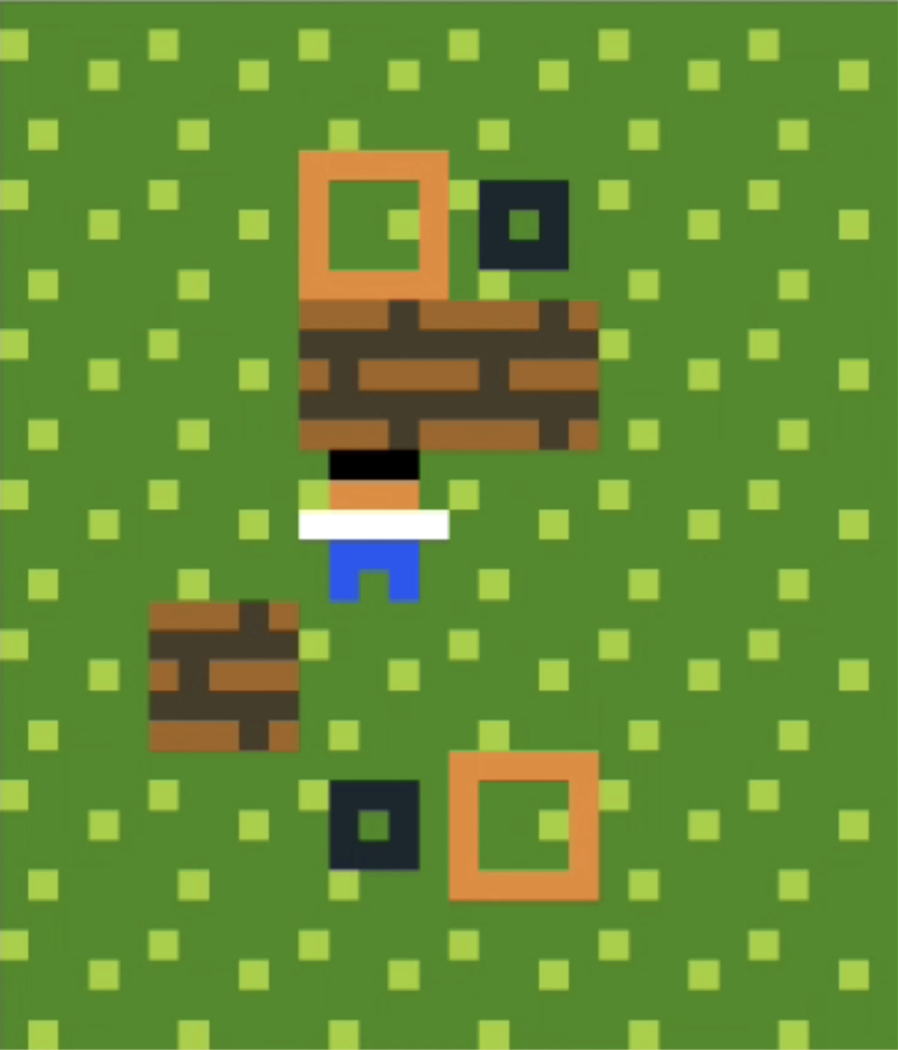
\includegraphics[width=\textwidth]{figures/windowdressingpart71.png} \hfill \\
\end{minipage}
$\Longrightarrow$
\begin{minipage}[t]{0.25\textwidth}
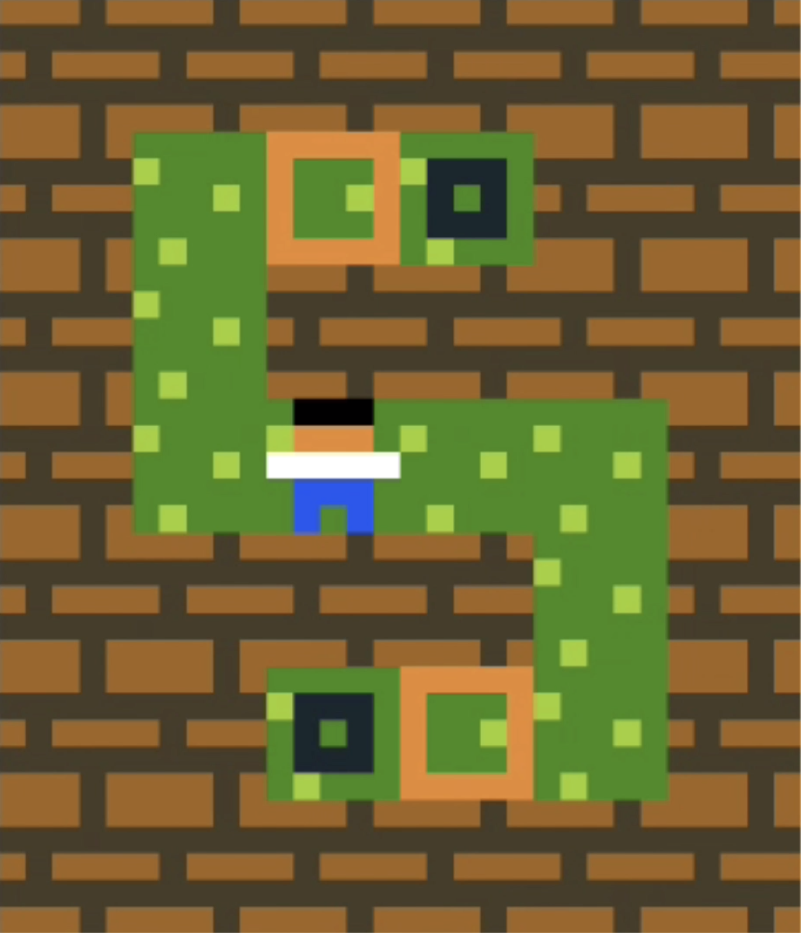
\includegraphics[width=\textwidth]{figures/windowdressingpart72.png} \hfill \\
\end{minipage}
$\Longrightarrow$
\begin{minipage}[t]{0.25\textwidth}
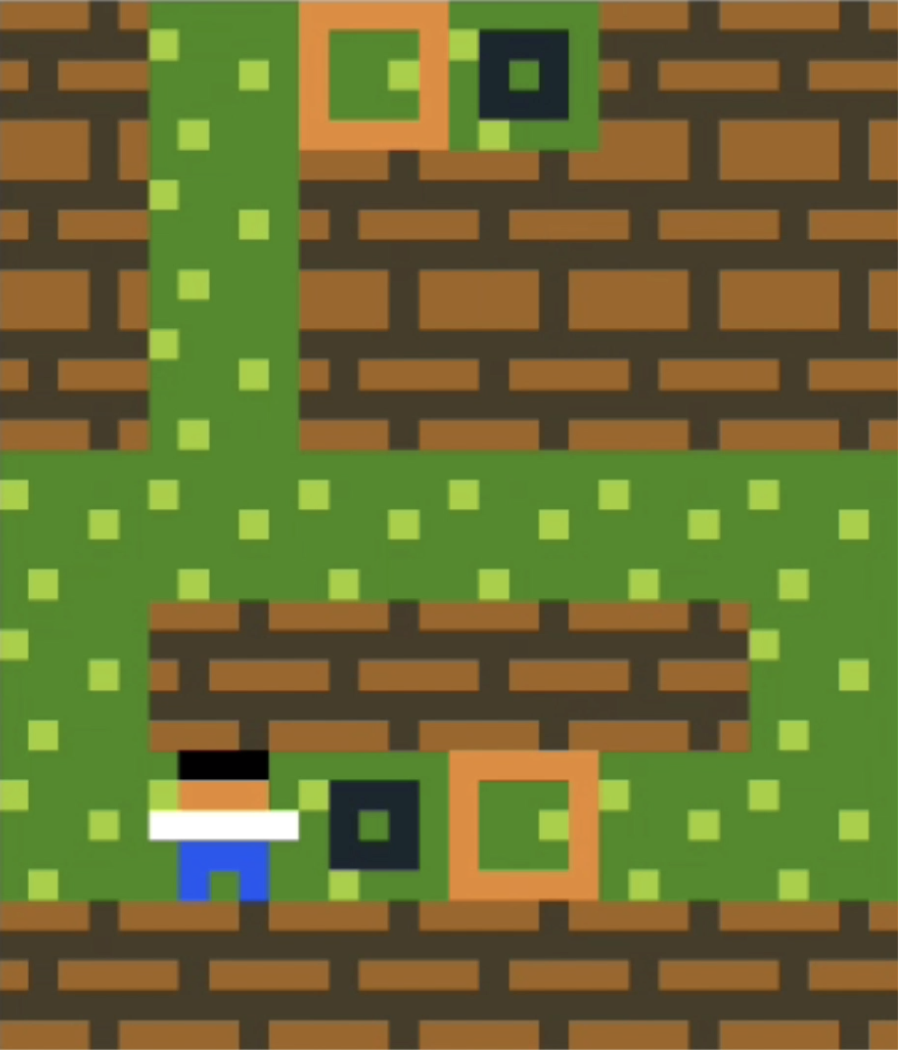
\includegraphics[width=\textwidth]{figures/windowdressingpart73.png} \hfill \\
\end{minipage}
\caption{Participant 7: Window dressing}
\end{figure}
    

\item[Mechanic swapping] Participant 1 already had a large library of Sokoban-like PuzzleScript games and used this to utilize the tool in an interesting manner. He loaded up a list of Sokoban levels into the tool and then started to change the rules of the Sokoban game. For example, he made it so you can push the block vertically put teleport through the block horizontally. After doing this, the tool quickly showed him the solvability of these levels under the new rules and allowed him to find novel solutions quickly.

\begin{figure}[!htbp]
\begin{minipage}{0.5\textwidth}
\centering
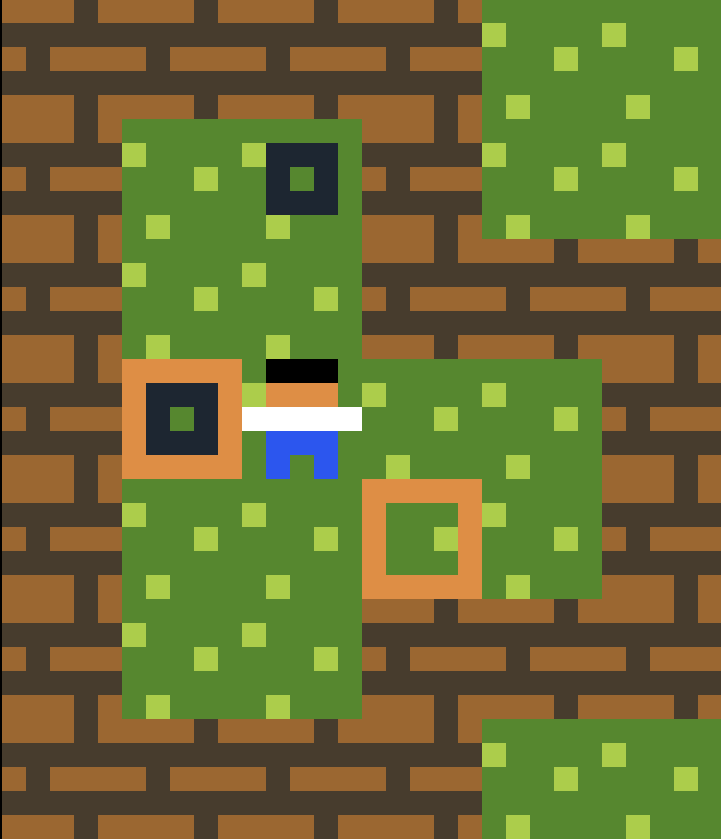
\includegraphics[width=0.7\textwidth]{figures/rulebasedimprovingfrom.png}
\end{minipage}  $\Longrightarrow$ \hfill
\begin{minipage}{0.5\textwidth}
\centering
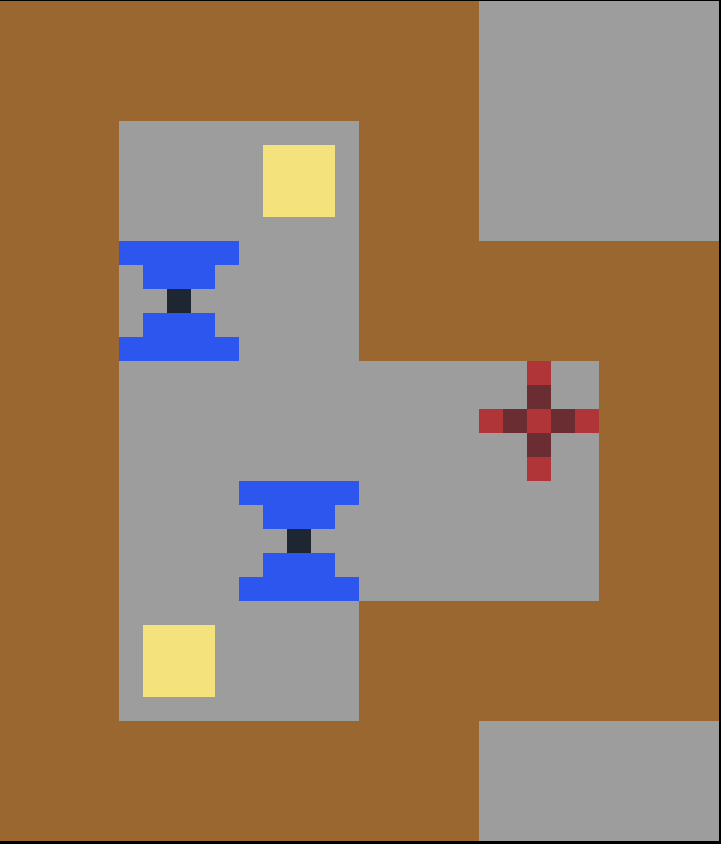
\includegraphics[width=0.7\textwidth]{figures/rulebasedimprovingto.png}
\end{minipage}
\caption{Participant 1: Mechanic swapping}
\end{figure}

% Show increpares level that looked like a classical sokoban level

\item[Gauging completeness] During the iterative design process participant 6 mentioned that he found the suggestions to be a useful stopping criterion. As soon as the suggestions did not improve the level in surprising ways, he would feel confident enough to stop iterating on the level further.

\textit{\say{Yes, especially as a level of confidence so I was sure that the current design was pretty solid when the suggestions seemed worse.}}
\end{description}

\subsection{Adapting to the transformer}
% why that's good, why there is not 'one-design method', only one of many such tools 
Every participant did, to some degree, modify their approach towards designing puzzle levels to incorporate the transformer. While our main focus was on how we can support the user in their design process of designing puzzle levels, some participants changed their approach towards designing puzzle levels significantly in order to exploit the strengths of the transformer.

We saw a clear difference of the perceived usefulness of the tool depending on which role the tool took in the design process.

Take as an example participant 5's approach when designing puzzle levels: \\
\hspace{\dimexpr-\fboxrule-\fboxsep\relax}\fbox{%
\begin{minipage}{\textwidth}
Participant 5 first decided that his Sokoban design should be created from an empty but large field. From there, he placed a few crates and walls but quickly noticed that the tool did not find interesting transformations. This was partially because our initial settings of the transformer only added a few walls on average making almost all levels trivial but requiring a lot of pushing around (making the solver believe that the level is difficult).

He then added more crates and targets believing that it would relinquish this error, but now the complexity of solving a single transformed level was upwards of 20 seconds.

Thinking that it takes too long to solve a single instance of a level he then added walls around the level, which should have helped to reduce the time it took to solve a single transformed level but this allowed for more unsolvable levels which were difficult to prove unsolvable.

Lastly, he manually added a wall on the top of the level, making the level significantly more difficult to his surprise.
\end{minipage}
}


Participant 5 tried to fit the tool into his method of designing puzzle games. In the beginning, he decided he would make a large Sokoban level with a lot of crates and reluctantly changed his plans after realizing that the tool did not do so well with these kinds of levels.

Participant 1 meanwhile had a few ideas at what MixedAim might be good at and simply tried to find the most interesting interactions with the tool and thus did not mind changing his approach towards designing puzzle levels.

The other participants fell somewhere in between, participants 2,3,6 \& 7 used MixedAim mostly in the way we intended it to be used and did not have to significantly adapt their design approach while using the tool. Participant 4 also tried to fit the tool in his method of designing puzzle games but with success, see the backward design section for more.

These different ways of adapting to mixed-initiative tools have also been mentioned by \cite{Guzdial}, who identified a few types of participants themselves.
One group of their participants attempted to fit every suggestion their AI made into a level, something we did not encounter, and other groups of participants who adapted their behavior to discover how best to interact with the tool, similarly to participant 1.

\begin{figure}[!htbp]
\centering
\begin{minipage}[t]{0.25\textwidth}
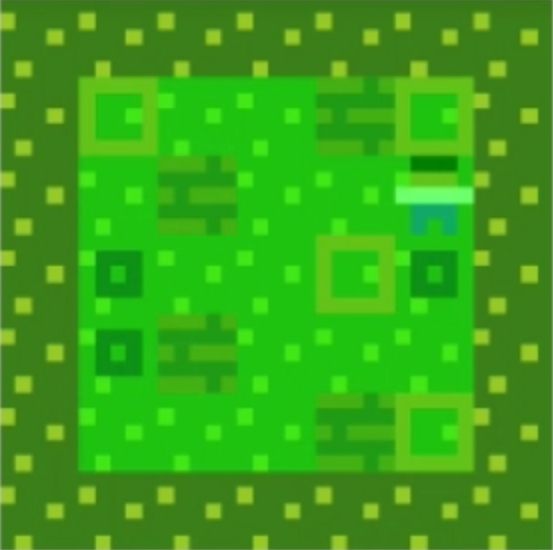
\includegraphics[width=\textwidth]{figures/part5i1_cropped.png} \hfill \\
\end{minipage}
$\Longrightarrow$
\begin{minipage}[t]{0.25\textwidth}
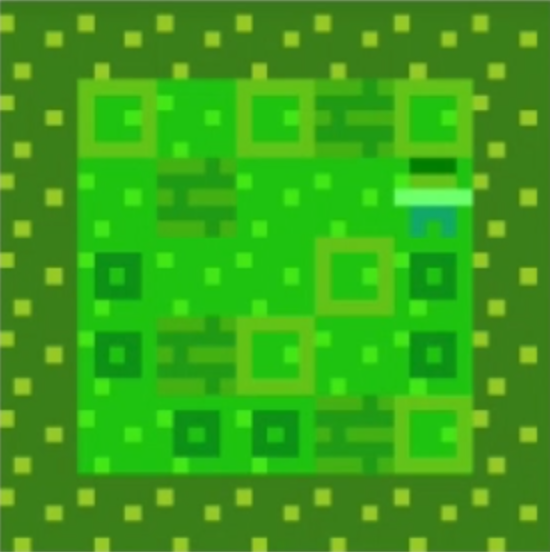
\includegraphics[width=\textwidth]{figures/part5i2_cropped.png} \hfill \\
\end{minipage}
$\Longrightarrow$
\begin{minipage}[t]{0.25\textwidth}
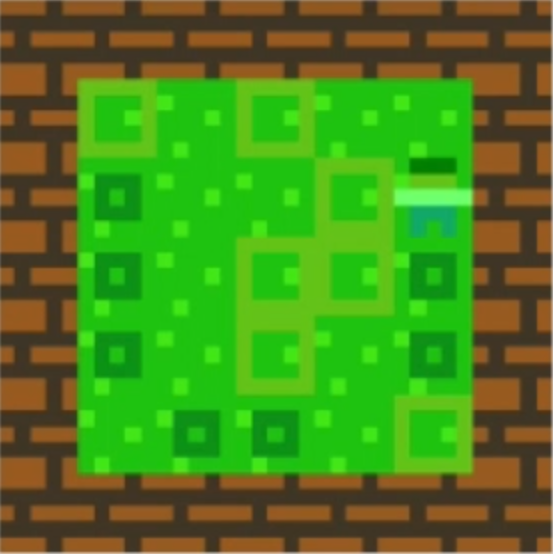
\includegraphics[width=\textwidth]{figures/part5i3_cropped.png} \hfill \\
\end{minipage}
$\Longrightarrow$
\begin{minipage}[t]{0.25\textwidth}
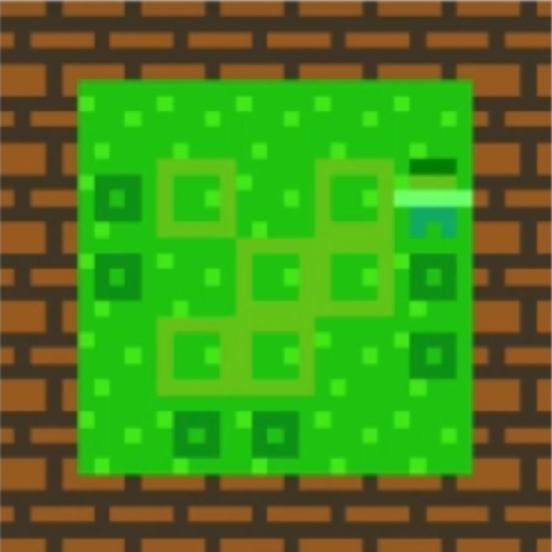
\includegraphics[width=\textwidth]{figures/part5i4_cropped.png} \hfill \\
\end{minipage}
$\Longrightarrow$
\begin{minipage}[t]{0.25\textwidth}
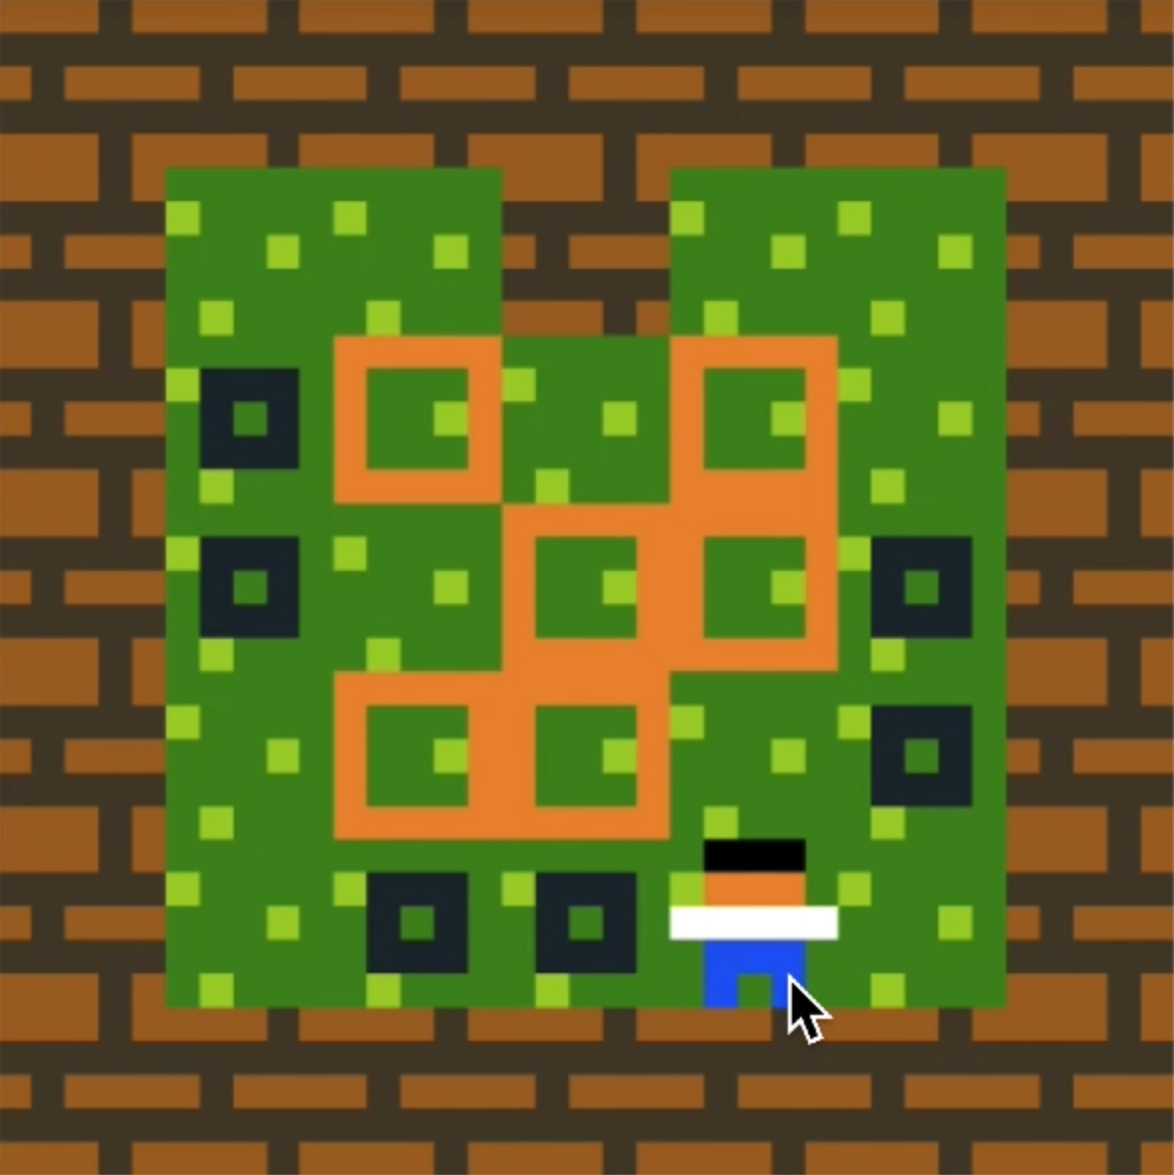
\includegraphics[width=\textwidth]{figures/part5i5.png} \hfill \\
\end{minipage}
\caption{Participant 5: Adaptive design process}
\end{figure}


We identified the following adaptions in the way users designed levels and provide a measure for judging the usefulness of an adaption based on one of these findings.


% \textbf{SUGGEST TO DISPLAY THESE FACTORS WHILE DESIGNING!!!!}

% 'What can be done' attitude vs. 'how can i fit the tool into my workflow'

%If a game designer had one way he would usually make puzzles and tried to fit their method onto the tool it could lead to issues. 

%We believe this might be because more experienced developers either tried to fit their method onto the tool (with varying degrees of success) or started to simply play around with the tool to exploit all the possible ways of creating levels.

% Under this model we also suggest a testable hypothesis to test interesting transformers. At the end we attempt to show a few rules of thumb that make it easy for the designer to implement such rules.



\begin{description}

    \item[Threshold-based searching] 
%Participant 1 \& 2 primarily used the transformer to identify interesting mechanics.
Participant 1 mentioned that there is a \textit{threshold} in the difficulty scores starting from which the levels become \textit{interesting}. This made him quickly change the level or the transformation rules until interesting suggestions appeared. As soon as they did, he then waited for more suggestions to appear.

\textit{\say{[...] there seems to be a threshold starting from which the levels get interesting, at least that's how it feels like qualitatively.}}

The other participants, though not stating this explicitly, acted similarly, swiftly changing the transformation rules until interesting levels occurred. When they occurred, they waited for more. For example, participant 5 frequently mentioned that the levels do not look difficult and quickly changed the transformation rules or the level until good suggestions came along.

    This threshold is entirely dependent on the level as the difficulty does not always correlate well with the perceived difficulty of the designer, something which was frequently mentioned (see negative feedback section). Sometimes this threshold is not reached due to it being difficult to solve the levels in time or because no interesting levels exist in the transformation but as soon as the threshold is reached practically all the levels are interesting.    

    With this insight we can model the usefulness of a transformation as the throughput of levels above this difficulty threshold.
\begin{equation}
\text{usefulness of transformation} = \frac{1}{\text{avg. time for interesting level}}
\label{eq:transformationusefulness}
\end{equation}
    
\begin{equation}
\text{avg. time for interesting level} = \left(1 - \frac{\text{\# interesting/difficult transformed levels}}{\text{\# total transformed levels}} \right) \cdot \text{avg. solve time}
\label{eq:transformationusefulness}
\end{equation}

    \item[Freezing sections] Participant 3 and 5 (among others) have chosen to freeze a few sections in the level, not because they necessarily thought they found these sections interesting, but to skew the search space to contain more interesting levels. For example participant 3 said quote \textit{\say{let me help it a little}} when he froze parts of the transformer section, see figure \ref{fig:part3shelp}.
    
    This adaption increases the throughput by increasing $\frac{\text{\# interesting difficult transformed levels}}{\text{\# total transformed levels}}$.
        
\begin{figure}
\centering
\begin{minipage}[t]{0.3\textwidth}
\includegraphics[width=\textwidth]{figures/part3helpalittlefrom.png} \\
\end{minipage}
$\Longrightarrow$
\begin{minipage}[t]{0.3\textwidth}
\includegraphics[width=\textwidth]{figures/part3helpalittleto.png} \\
\end{minipage}
\caption{Participant 3 freezing sections to aid the transformer\label{fig:part3shelp}}
\end{figure}

    
    \item[Smaller levels] Participant 1 concluded that the transformer is well-suited to create small Sokoban levels, see figure \ref{fig:part1smallsokoban}. He also experimented with variations of Sokoban rules and created a few puzzle games with small levels using this method (\href{https://www.increpare.com/game/all-green-to-blue.html}{'All Green To Blue'}\footnote{https://www.increpare.com/game/all-green-to-blue.html} and \href{https://www.increpare.com/game/all-green-and-blue-on-yellow.html}{'All Green To Blue On Yellow'}\footnote{https://www.increpare.com/game/all-green-and-blue-on-yellow.html} which you can play online), see figure \ref{fig:part1smalllevelgames}.
    
    This adaption increases the throughput by increasing the \textit{average time for solving a transformed level}.
    
    
    \begin{figure}
\centering
\includegraphics[width=\textwidth]{figures/part1_smallsokobandesigns.png}
\caption{Participant 1's small Sokoban transformations \label{fig:part1smallsokoban}}
\end{figure}


\begin{figure}
\centering
\begin{minipage}[t]{0.3\textwidth}
\includegraphics[width=\textwidth]{figures/part1AllGreenToBlue.png} \\
\end{minipage}

\begin{minipage}[t]{0.3\textwidth}
\includegraphics[width=\textwidth]{figures/part1allgreentoblueonyellow.png} \\
\end{minipage}
\caption{Participant 1's custom games \label{fig:part1smalllevelgames}}
\end{figure}

    \item[Larger levels] Participant 5 decided that larger levels would be better for the transformer because it would allow for a larger quantity of interesting levels. However, this approach also allows for more uninteresting levels and significantly decreased the \textit{average time for solving a transformed level}, which made choosing larger levels a bad adaption to the system.
    
    \item[More variation] Lastly, we observed that some games are better suited for identifying interesting mechanics than others. Both we and participant 2 have had such success with puzzle games that feature polyominoes.

This leads us to believe that Sokoban-like puzzle games with large variations in a small space are especially well-suited for identifying interesting mechanics. When focusing on small levels it does not take a lot of time to find a solution or prove that no solution exists and would take at most in the order of $\mathcal{O}\left( {n^2 \choose a} \right)$ computational steps, where $a$ are the number of blocks in the generated level and $n^2$ are the possible places the blocks can be placed. Notice that using a variety of different objects (for example differently shaped polyominoes) does not change the value of $a$. Thus one can build more interesting small levels with puzzle games that have a lot of different types and shapes of objects, as opposed to games with only three types of $1 \times 1$ objects. 

% \item[Structural changes] 


\end{description}

\iffalse
We identified a few rules of thumb that happen to apply to all of our three solvers:
\begin{itemize}
\item Large levels can have a lot of moving around before solving a level which makes many levels difficult for the solvers (but not necessarily interesting).
\item A level with lots of crate/target pairs in Sokoban has more combinations and would take a lot of time to solve.
\item A sparse Sokoban level only has a small fraction of interesting levels.
\item A dense Sokoban level is more likely to be unsolvable and would take the solver a lot of time to show that no solution exists.
\end{itemize}
\fi

\subsection{Backward designing}

\begin{figure}
\centering
\includegraphics[width=.85\textwidth]{figures/backward_design_minotalen.png}
\caption{Backward design of participant 4's puzzle game\label{fig:backwarddesign}}
\end{figure}

This method of designing levels with the mixed-initiative system was discovered and coined by participant 4 and was not foreseen in the original research question. In backward design, you start to design a level from a solved state and slowly turn it into a more complicated/interesting, but always solvable, level.
Participant 4 used it specifically for their PuzzleScript game \ref{fig:backwarddesign} but this backward approach can also be used for Sokoban. 

% Participant 4 used it on a block expanding level 

Both \cite{Taylor2011} and \cite{Kartal2015} have employed such a backward design approach for generating Sokoban levels. We will now illustrate how their approaches can be formulated as transformer rules in MixedAim with which designers could interactively backward design.

\begin{description}
\item[\cite{Taylor2011}] This assumes that the target positions are fixed and no crates are in the initial design. The player then pulls the crates away from the goal.
\begin{lstlisting}
(place crates on all targets)
[Target No Crate] -> [Target Crate]
(move the player around and let him pull crates)
choose 50 [Player | No Obstacle] -> [| Player]
or [No Obstacle | Player | Crate] -> [Player | Crate | ]    
\end{lstlisting}

\item[\cite{Kartal2015}] This assumes that the crate positions are fixed and no targets are in the initial design. The player then pushes the crates around and at the end turns them into targets.

\begin{lstlisting}
(add a placeholder to all crates)
[Crate] -> [Crate Placeholder]
(move the player around and let him push crates)
choose 50 [Player | No Obstacle] -> [ | Player]
or [Player | Crate | No Obstacle] -> [ | Player | Crate] 
(replace crates with targets and placeholders with crates)
[Crate] -> [Target]
[Placeholder] -> [Crate]
\end{lstlisting}
\end{description}

\section{Structured Interview Responses}

For most participants, we took the structured interview immediately after the think-aloud study, depending on the preference in writing or orally. Participants 1 and 4 did the structured interview after using the tool for a few days testing it not only on Sokoban but also on their games. Since the questions are quite open-ended, we would just skip a few of them if the participant had already answered them in a previous question. 

We compiled a list of the most interesting answers to the questions in the appendix \cite{apx:interview} but believe that the most important insights from the interviews have either been mentioned or are elaborated in the next sections.



\section{Negative feedback}

Unfortunately, not all participants had a very smooth experience with the tool. Especially participant 5 immediately decided that interesting Sokoban levels were large and would contain a lot of crates which unfortunately the transformer did not handle very well. The designer then had to limit himself to designs that the transformer supported better.

He also admitted that while making levels with the tool can be more efficient, passively showing information can take the fun out of solving the level and one might be easily attempted to just look at the solution instead of working it out in the head \ref{fig:part5comments}.

Participant 6 addressed the same concern mentioning that there is a `Google effect' that makes him stop thinking about solvability (Google effect meaning that people do not attempt to remember a fact but instead remember how to look it up instead). He did not see this in a negative light though, and enjoyed that it made the process faster.

\begin{figure}
\begin{minipage}[t]{\textwidth}
\textit{\say{Part of designing a puzzle is trying to make the best puzzle you can make, but part of it is also the fun of solving intermediate states yourself. So that's one thing that I would miss with the software (you might be able to work around it) but one thing I like about designing puzzles, is to constantly be thinking about solutions in my head, so this is kind of giving this up a little bit, and I'm not actively thinking about solutions when I'm designing.}} \hfill \\

\textit{\say{I can create better puzzles with this tool but might have less fun while doing it.}}

\textit{\say{There's a kind of Google effect where I stop thinking about solvability.}}

\end{minipage}
\caption{Participant 5 \& 6's quotes regarding solvability\label{fig:part5comments}}
\end{figure}



Participant 1, who is very experienced with puzzle design, has a different mindset towards the transformer and just thinks that it adds another tool for inventing levels.

Participant 1 fears that designers who have not had a lot of manual puzzle-developing experience would end up making uninteresting levels, which are just `interesting enough' to put into a game. \cite{Guzdial} mentioned similar concerns that their tool could replicate an over-used design. This gives an additional responsibility to the designer, who now has to resist relying too much on the system.

Participant 1's quote sums it up nicely: 
\textit{\say{They're cool to work with [referencing the tools], but it's so easy to make bad and difficult levels (a fatal combo).}} % from tweet


% Additionally, there were a lot of user interface suggestions, like being able to hide the passive information on the current level, seeing how many levels have already been transformed, etc.

\section{Suggestions}

\begin{description}
    \item[Use more sophisticated curators / more accurate difficulty measure]
A very common complaint (every participant except for 1, 5 and 6 mentioned it) was that we curated levels based only on the difficulty of the solver and that the difficulty of the solver also does not always match the perceived difficulty.

\textit{\say{The limitations are [the systems] judging abilities.} -- Participant 3}

Due to time constraints, we decided from the beginning to keep the curator very simple. However, after interviewing participant 1 \& 4 we have a suggestion for future work to improve upon the curator. We suggest adding an optional `cost' modifier to operational rules. 

 For example: \lstinline{[ > Player | Crate ] -> [ > Player | > Crate ] COST 10} \hfill \\
 This way, levels that require more costly rules in order to be solved are given a higher difficulty score. The rule above would discourage levels that need a lot of moving around without pushing blocks.

% more pushing of blocks are weighted more and gives control to the designer and lets him implement their subjective experience of what makes a difficult puzzle game.
 

    \item[Feedback for adapting to the transformer]
    Participant 4 suggested showing how many levels have already been transformed to get an estimate of the effectiveness of the transformer.
    
    We suggest to take this a step further and also show the throughput of curated levels and also show how many levels are solvable/unsolvable/timed-out, respectively. These changes would allow the user to better adapt their actions towards the transformer. 
    
    \item[Unresponsiveness]
    A lot of participants felt like the transformer was unresponsive at times, due to there being no visual feedback when MixedAim found no suitable suggestions. Participant 4 \& 7 both suggested adding a button to explicitly generate the levels instead of automatically transforming them, while Participant 1 suggested labeling more clearly that the transformer was doing its work.
    
    \item[Improve UI] A suggestion by participant 5 was that the tool should have an option to enable/disable showing passive information about a level since knowing that a solution exists can tempt you to click on it instead of solving it yourself, which is an aspect he would otherwise miss when designing puzzle games.
     
     \item[Level progression aid] Participant 4 suggested that the tool should also help in deciding an interesting level progression sequence. This is far beyond the scope of our work. However, \cite{Butler2013} has promising work in this direction. 
    
\end{description}

\section{Conclusion}

We developed the mixed-initiative system MixedAim for creating PuzzleScript games interactively with the computer. For this purpose we generalized the Sokoban heuristic of \cite{Jurgen} to solve levels more efficiently, we crafted a user interface which supported various forms of direct manipulation, like using the level editor and playtesting a game and added support for interactive suggestions. We hypothesized and later confirmed that giving more difficult suggestions is a feasible way to assist the designer. Specifically, we have identified that there is a threshold in difficulty starting from which levels become interesting.

We identified various key interactions with those suggestions that designers and illustrated in which way designers could benefit from them. Interactions included \textit{Identifying and constraining mechanics and aesthetics in designs}, \textit{making unsolvable levels work again through transforming},  \textit{window dressing}, \textit{mechanic swapping}, \textit{gauging completeness} and \textit{backward designing}.

Furthermore, we analyzed how participants adapted to the MixedAim suggestions, identified that the perceived usefulness is dependent on the role of MixedAim in the design process and noticed that it was particularly good at identifying interesting mechanics in small levels with large variations.

Through the user interviews, we identified that some designers experienced a `Google effect' that made users delegate the responsibility of solving the level to the MixedAim system. Some view this as taking out the fun, while others simply think this is efficient. Lastly, we also received concerns that the tool can make it easy to create difficult and bad levels which give additional responsibility to the designer planning to incorporate such tools in their workflow.

Overall, we believe that mixed-initiative methods add value to the design process if they are approached as just another tool in the toolset for creating puzzle games and not as the de facto replacement of one's usual design process.

% !TEX root = ../thesis.tex
\iffalse
\chapter{Outlook}

We feel this deserves a separate chapter as our study was primarily a qualitative study on game design. 



Lorem ipsum dolor sit amet, consectetuer adipiscing elit, sed diam nonummy nibh euismod tincidunt ut laoreet dolore magna aliquam erat volutpat. Ut wisi enim ad minim veniam, quis nostrud exerci tation ullamcorper suscipit lobortis nisl ut aliquip ex ea commodo consequat. Duis autem vel eum iriure dolor in hendrerit in vulputate velit esse molestie consequat, vel illum dolore eu feugiat nulla facilisis at vero et accumsan et iusto odio dignissim qui blandit praesent luptatum zzril delenit augue duis dolore te feugait nulla facilisi. Lorem ipsum dolor sit amet, consectetuer adipiscing elit, sed diam nonummy nibh euismod tincidunt ut laoreet dolore magna aliquam erat volutpat. Ut wisi enim ad minim veniam, quis nostrud exerci tation ullamcorper suscipit lobortis nisl ut aliquip ex ea commodo consequat. Duis autem vel eum iriure dolor in hendrerit in vulputate velit esse molestie consequat, vel illum dolore eu feugiat nulla facilisis at vero et accumsan et iusto odio dignissim qui blandit

Lorem ipsum dolor sit amet, consectetuer adipiscing elit, sed diam nonummy nibh euismod tincidunt ut laoreet dolore magna aliquam erat volutpat. Ut wisi enim ad minim veniam, quis nostrud exerci tation ullamcorper suscipit lobortis nisl ut aliquip ex ea commodo consequat. Duis autem vel eum iriure dolor in hendrerit in vulputate velit esse molestie consequat, vel illum dolore eu feugiat nulla facilisis at vero et accumsan et iusto odio dignissim qui blandit praesent luptatum zzril delenit augue duis dolore te feugait nulla facilisi. Lorem ipsum dolor sit amet, consectetuer adipiscing elit, sed diam nonummy nibh euismod tincidunt ut laoreet dolore magna aliquam erat volutpat. Ut wisi enim ad minim veniam, quis nostrud exerci tation ullamcorper suscipit lobortis nisl ut aliquip ex ea commodo consequat. Duis autem vel eum iriure dolor in hendrerit in vulputate velit esse molestie consequat, vel illum dolore eu feugiat nulla facilisis at vero et accumsan et iusto odio dignissim qui blandit
Lorem ipsum dolor sit amet, consectetuer adipiscing elit, sed diam nonummy nibh euismod tincidunt ut laoreet dolore magna aliquam erat volutpat. Ut wisi enim ad minim veniam, quis nostrud exerci tation ullamcorper suscipit lobortis nisl ut aliquip ex ea commodo consequat. Duis autem vel eum iriure dolor in hendrerit in vulputate velit esse molestie consequat, vel illum dolore eu feugiat nulla facilisis at vero et accumsan et iusto odio dignissim qui blandit praesent luptatum zzril delenit augue duis dolore te feugait nulla facilisi. Lorem ipsum dolor sit amet, consectetuer adipiscing elit, sed diam nonummy nibh euismod tincidunt ut laoreet dolore magna aliquam erat volutpat. Ut wisi enim ad minim veniam, quis nostrud exerci tation ullamcorper suscipit lobortis nisl ut aliquip ex ea commodo consequat. Duis autem vel eum iriure dolor in hendrerit in vulputate velit esse molestie consequat, vel illum dolore eu feugiat nulla facilisis at vero et accumsan et iusto odio dignissim qui blandit

Lorem ipsum dolor sit amet, consectetuer adipiscing elit, sed diam nonummy nibh euismod tincidunt ut laoreet dolore magna aliquam erat volutpat. Ut wisi enim ad minim veniam, quis nostrud exerci tation ullamcorper suscipit lobortis nisl ut aliquip ex ea commodo consequat. Duis autem vel eum iriure dolor in hendrerit in vulputate velit esse molestie consequat, vel illum dolore eu feugiat nulla facilisis at vero et accumsan et iusto odio dignissim qui blandit praesent luptatum zzril delenit augue duis dolore te feugait nulla facilisi. Lorem ipsum dolor sit amet, consectetuer adipiscing elit, sed diam nonummy nibh euismod tincidunt ut laoreet dolore magna aliquam erat volutpat. Ut wisi enim ad minim veniam, quis nostrud exerci tation ullamcorper suscipit lobortis nisl ut aliquip ex ea commodo consequat. Duis autem vel eum iriure dolor in hendrerit in vulputate velit esse molestie consequat, vel illum dolore eu feugiat nulla facilisis at vero et accumsan et iusto odio dignissim qui blandit
\fi


% ---- END MAIN PART ----

\clearpage
\appendix
\clearpage
\renewcommand*{\chapterpagestyle}{myappendixpagestyle}

% !TEX root = ../thesis.tex

\chapter{Information For The Few (Appendix)}

\section{Needfinding survey}
\label{needfindingq1}
\begin{description}
	\item[Why do people play puzzle games?] \hfill \\
	\textit{"to feel smart", "experience aha-moments", "increased spatial reasoning skills", "to get into the state of flow", "because it is fun"}	
	\item[What's the hardest aspect about making puzzle games?] \hfill \\
	\textit{"Deciding whether the mechanics are fun.", "Completeness. Having confidence that you fully explored the possibility space of a mechanic is daunting.", "Finding a balance between completeness and drawing a strong boundary around the concept.", "Creating a set of puzzle mechanics that's elegant, uses as little elements as possible in as many as possible interesting combinations, and generating a puzzle set that's both sufficent in quality and quantity."}
	
	\item[In which way do you hope automated tools will help design puzzle games?]
	\textit{"Finding novel configurations and solutions.",  "For creative inspiration. Finding ideas that a person would have trouble discovering.", "Mostly to help speed up finding puzzles that might have certain properties, or to allow me to experience types of puzzles I might not normally have designed on my own.", "Reduce hand work on the designer, so that the designer can focus more on improving the mechanics and increasing the set of puzzles."}
	\end{description}


\begin{figure}
    \centering
    %\setlength{\tabcolsep}{0.5\linewidth}
    \includegraphics[width=1.0\linewidth]{figures/whichtoolsemployduringleveldesign.png}
    
    \caption[Needfinding]{Needfinding survey Q3 %
    \label{fig:needfindingq3}}
\end{figure}

% \includepdf[pages=-]{needfindingsurvey.pdf}

\section{PuzzleScript}

\begin{figure}
\centering
\begin{lstlisting}[language=PuzzleScript]
========
OBJECTS
========
Background
LIGHTGREEN

Target
DarkBlue

Wall
BROWN

Player
White

Crate
Orange

=======
LEGEND
=======
. = Background
# = Wall
P = Player
* = Crate
@ = Crate and Target
O = Target

=======
SOUNDS
=======
Crate MOVE 36772507

================
COLLISIONLAYERS
================
Background
Target
Player"Wall"Crate

======
RULES
======
[ >  Player | Crate ] -> [  >  Player | > Crate  ]

==============
WINCONDITIONS
==============
All Crate on Target

=======
LEVELS
=======
####..
#.O#..
#..###
#@P..#
#..*.#
#..###
####..
\end{lstlisting}
    \caption[Sokoban]{Example Sokoban implementation in PuzzleScript %
    \label{fig:sokobaninpuzzlescript}}
\end{figure}


\begin{figure}
\includegraphics[width=1.0\linewidth]{figures/RULE_EXPANDED.png}
\caption[BNF Diagram]{ BNF Diagram for a PuzzleScript rule \textsuperscript{a)}\label{fig:puzzlescriptrulebnf}}
\small\textsuperscript{a)} Note that matched\_Property has to be a property that either appears only once on the left-hand side or a property that is exactly at the same location on the left-hand side. Whatever property it matches will be replaced on the right-hand side.
\end{figure}
\footnote{Note that matched\_Property has to be a property that either appears only once on the left-hand side or a property that is exactly at the same location where the property appears on the left-hand side. Whatever property it matches will be replaced on the right-hand side.}

\newpage


\section{User study}

\begin{sidewaystable}
\small
\begin{tabular}[t]{l||c|c|c|c|c|c|c}
\toprule
% Participant &  Stephen 1 & Marcos 2 & ThatScar 3 & 4 Minotalen & 5 Joel & 6 Max & Sam 7 \\
Participant &  1 & 2 & 3 & 4 & 5 & 6 & 7 \\
\midrule
Age & 34 & 46 & 20 & 25 & 30 & 27 & 28 \\
Gender & male & male & male & trans & male & male & male \\
Profession & game designer & \specialcell[t]{programmer \& \\ game designer} & junior programmer & design student & doctor & game designer & game designer \\
Puzzle Design Experience & 15 years & 8 years & 3 years on and off & 1 year, 3 games & 1 year, 200 hours & \specialcell[t]{2 days \\ 5 years (gd)} & 4 years \\
%How to design & Not quickly.  I've used a bazillion different techniques (on paper sometimes, in level editors with various levels of assistence, to fully autogenerated). &  &  . & forward design & fidn interesting geometry \\
\bottomrule
\end{tabular}
\caption{Demography of user study\label{tab:demography}}
\end{sidewaystable}


\section{Structured interview questions\label{apx:interview}}

This is a compiled list of the most interesting answers to the interview questions:


\textbf{Tell me about your experience with the editor.}

\textit{\say{In broad terms it does some cool things. Bunch of usability suggestions. I have to figure out more use cases.} -- Participant 1}

\textit{\say{Overall it's a very interesting project. Some quirks of the interface are to be solved but I hope you can expand it and make it more powerful.} -- Participant 2}

\textit{\say{The editor was fun to use, but oftentimes I found it was lacking visual feedback of the ongoing generation process.} -- Participant 4}

\textbf{How was this design process different from your usual practice?}

\textit{\say{Designing with a level generator gives the advantage of encountering new object 'constellations' that are sometimes unintuitive and difficult to solve.} -- Participant 4}

\textit{\say{Faster, felt like communication, not trivial.} -- Participant 6}

\textit{\say{The loop of mutating/trying/repeat is very appealing, reminiscent to genetic art generators. Usually I make a loop of generating/curating/repeat for my games, perhaps this type of tool can insert a very useful step with the mutator.} -- Participant 2}

\textbf{How satisfied are you with the design(s)?}

\textit{\say{Some of the levels I found are very surprising and pleasing.} -- Participant 2}

\textit{\say{I wasn't happy with the designs (of the Sokoban levels) but attribute that mainly to my error, could have used a more interesting generation algorithm and level base. Sokoban levels have been generated for ages, so my levels were probably not original. Maybe going with a different base game (block pulling maybe?) would have resulted in more originality.} -- Participant 4}

\textit{\say{The levels are already quite neat! I'd say about 20\% were really interesting.} -- Participant 6}

\textit{\say{Not particularly.} -- Participant 5}

\textbf{How original do you think are the levels?}

\textit{\say{Not really. There should be more curated suggestion levels.} -- Participant 6}

\textbf{Did the functionalities hinder you to do anything and if yes what was it?}

\textit{\say{I did more than I imagined I could with the tool.} -- Participant 3}

\textit{\say{Some elements of the interface are difficult to understand at first, and some others are difficult to use, like the text editor.} -- Participant 1}

\textit{\say{The editor had most of the functionality that it needs, some 'quality of level' improvements would be required to tie it all together though. Not being able to alter level size from within the editor was annoying, also the Transform text box clearing on tab switch was a hindrance. Not being able to alter level size from within the editor was annoying, also the Transform text box clearing on tab switch was a hindrance.} -- Participant 4}

\textit{\say{I was able to do more in a short amount of time and check more things than I would usually.} -- Participant 6}

\textbf{Can you tell me how you experienced the interaction with the editor?}

\textit{\say{I used mainly the mouse, and some of the suggested shortcuts. I did not try to use the text editor very much.} -- Participant 2}

\textit{\say{Without the verbal confirmation that the generator is working I'd have believed it was not generating and kept restarting the process. Otherwise it was mostly fine.} -- Participant 4}

\textit{\say{It felt like a communication with the exception of the things I controlled.} -- Participant 6} (Note: This participant only used the suggested buttons and did not implement his own transformation rules).

\textit{\say{Watching numbers go up and gradually in the transformer and if it's too slow i'll change the transforms and fiddle with the level size. The polishing at the end I do by hand.}  -- Participant 1}

\textbf{How useful were the suggestions by the system? How did they help you?}

\textit{\say{The mutations were generally chaotic, but some of them were surprising, apparently impossible to solve, hence very fun to solve.} -- Participant 2}

\textit{\say{The level suggestions were as useful as the generation rules I fed into the system. The suggestions can be helpful for coming up with own design ideas.} -- Participant 4}

\textbf{Did you think that the system pointed you in different directions than you intended?}

\textit{\say{If the purpose of the system is generating new ideas, then new ideas would be an intended direction, so no.} -- Participant 4}

\textit{\say{I was just trying to figure out what the tool can and cannot do.} -- Participant 1}

\textit{\say{Not much, only worked well on smaller sized levels.} -- Participant 5}

\textbf{In your view, how did the system make the suggestions?}

\textit{\say{I suspect the system uses digital mutation operations that modify the current element of the levels, and tries to solve the new levels, discarding unsolvable/trivial ones.} -- Participant 2}

\textit{\say{It made the suggestions based on the results of my transformation rules, a solver and a complexity rating algorithm.} -- Participant 4}

\textbf{Can you reflect on how your behaviour impacted the suggestions of the system?}

\textit{\say{I feel that the selection of levels from me reinforces the kind of variations the system makes later.} -- Participant 2}

\textit{\say{The transformation rules directly impact what levels are generated, the solvable subset of those gets rated by complexity, the four highest-razed levels get presented to me, so the impact of the rules is indirect.} -- Participant 4}

\textit{\say{Well I kind of knew what it did after you explained it so it just did what I wanted it to do.} -- Participant 6}

\textit{\say{The modify and leave buttons impacted it.} -- Participant 3} 

\textbf{How much did you feel the system understood your aim?}

\textit{\say{I feel like in its current state the system does not use all the feedback loops it could use.} -- Participant 2}

\textit{\say{The system has the aim of creating complex levels from a set of rules. Formulating intentions would happen by setting rules and base level but the system would not 'understand', just process.} -- Participant 4}

\textit{\say{Pretty well.} -- Participant 1} % I'm learning what the system can do to get an idea how it works

\textit{\say{It didn't really \say{understand} it since it's just a tool.} -- Participant 3}

\textit{\say{It is not intelligent, it just did what I told it to do and it was a useful tool.} -- Participant 6}

\textbf{How would you characterise the tool within the design process?}

\textit{\say{As an integral part, like a canvas where experiment within the level space.} -- Participant 2}

\textit{\say{Perhaps useful for coming up with variations and unintuitive level designs.} -- Participant 4}

\textit{\say{The role of saving levels, playing them, checking if they are solvable and finding their solutions if so. Additionally, it brought me ideas and did its job quite well.} -- Participant 6}

\textit{\say{I don't have a loop of iterative design, I'm just looking for a good starting point.
The suggestions are nice and interesting.} -- Participant 1}

\textbf{How well did the scores for the difficulty of the level match your estimation?}

\textit{\say{Good enough to be useful, but somewhat uneven. I believe the system could integrate more evaluation criteria to make the estimation more exact.} -- Participant 2}

\textit{\say{Difficulty rating did not align with my perception of difficulty, but I've not yet explored enough to be sure.} -- Participant 4}

\textit{\say{I did not look at the difficulty scores, just at the curated levels.} -- Participant 6}

\textit{\say{Pretty accurate, there seems to be a threshold starting from which the levels get interesting, at least that's how it feels like qualitatively.} -- Participant 1}

\textbf{Did a suggestion inspire you without you clicking on it?}

\textit{\say{Yea, exactly what happened in the end.} -- Participant 3}

\textit{\say{Yes, especially as a level of confidence so I was sure that the current design was pretty solid when the suggestions seemed worse.} -- Participant 6}

\textit{\say{No, but could happen. Looking at them and trying to solve them in the head is slower than just clicking on them to try it out.} -- Participant 1}

Note: The people who said no were simply adapt at quickly trying out a suggestion and popping back to the old design.

\textbf{Would you use such a system in your work practice and when? 
If Yes: What for in specific; If No: What needs to be changed?}

\textit{\say{I would use it to find new levels for my games, but also to inspire my level generators with some kind of variations I usually don't explore because lack of real time visualisation.} -- Participant 2}

\textit{\say{Yes, for creating level states that I hadn't encountered before, then using those as inspiration.} -- Participant 4}

\textit{\say{Not for the game I'm currently working on but if I design a puzzle game in the future again sure.} -- Participant 6}

\textit{\say{Yea, for certain particular games. Also for super compact levels on any kind of puzzle game.} -- Participant 1}

\textbf{Where do you see the potential of such systems and where the limitation?}

\textit{\say{There is great potential to explore rule variation in addition to level variation. Limitations are, like always, memory and cpu usage when using mutators and solvers not tuned to specific rules.} -- Participant 2}

\textit{\say{Potential for creating unintuitive and thus hard to solve levels. Potential for improving handmade levels. Limitation in  complexity heuristics and level size (since computation effort increases exponentially)} -- Participant 3}

\textit{\say{Potential is to create low effort levels and it allows you to constrain your creativity. There's a kind of Google effect where I stop thinking about solvability. Probably if you've been designing puzzles for a specific game for a long period of time the tool probably won't help much anymore, so it's more useful in the prototype phase. The limits are the language of PuzzleScript and the language of the transformer.} -- Participant 4}

\textit{\say{Performance limitations. Level size, \# of rules, people making bad levels with it, people making levels that aren't fun. I'm always going to try to make small levels with it.} -- Participant 1}

\textit{\say{The limitations are [the systems] judging abilities.} -- Participant 3}

\textbf{Do you have any thoughts you would like to add?}

\textit{\say{I hope more kind of games are added later to the system (3D and/or continuous-like rules).
This project is very promising, I cannot wait to try the next version, and possibly contribute to it.} -- Participant 2}



\clearpage
\renewcommand*{\chapterpagestyle}{empty}

%\nocite{*}
\cleardoublepage
\phantomsection
\addcontentsline{toc}{chapter}{Bibliography}
\bibliography{graphics}

\end{document}
